\section{Mức độ 7,8 điểm}
\setcounter{ex}{0}
\setcounter{dang}{0}
\begin{dang}
    {Tìm tập xác định hàm số mũ - logarit}
\end{dang}
\Opensolutionfile{ans}[ans/CD18/Muc_7_8]
\begin{ex}%[2D2B4-1]
    [Mã 105 2017]
    Tìm tất cả các giá trị thực của tham số $m$ để hàm số $y=\log\left(x^2-2x-m+1\right)$ có tập xác định là $\mathbb{R}$.
    \choice
    {$m\le 2$}
    {$m>2$}
    {$m\ge 0$}
    {\True $m<0$}
    \loigiai{
        Để hàm số có tâp xác định $\mathbb{R}$ khi và chỉ khi $x^2-2x-m+1>0$, $\forall x\in\mathbb{R}$.\\
        $\Leftrightarrow{\Delta}'<0$ $\Leftrightarrow{\left(-1\right)^2}-1\cdot\left(-m+1\right)<0$ $\Leftrightarrow m<0$.
    }
\end{ex}

\begin{ex}%[2D2B4-1]
    [Mã 104 2017]
    Tìm tất cả các giá trị thực của tham số $m$ để hàm số $y=\ln \left(x^2-2x+m+1\right)$ có tập xác định là $\mathbb{R}$.
    \choice
    {$0<m<3$}
    {$m<-1$ hoặc $m>0$}
    {\True $m>0$}
    {$m=0$}
    \loigiai{
        Hàm số có tâp xác định $\mathbb{R}$ khi và chỉ khi $$x^2-2x+m+1>0,\forall x\in\mathbb{R}\Leftrightarrow\heva{
            &a=1>0 \,(\text{luôn đúng})\\
            &{\Delta}'=1-\left(1+m\right)<0\Leftrightarrow m>0.}$$
    }
\end{ex}

\begin{ex}%[2D2B4-1]
    Hàm số $y=\ln \left(x^2+mx+1\right)$ xác định với mọi giá trị của $x$ khi
    \choice
    {$\hoac{& m<-2\\& m>2}$}
    {$m>2$}
    {\True $-2<m<2$}
    {$m<2$}
    \loigiai{
        Yêu cầu bài toán $\Leftrightarrow x^2+mx+1>0$, $\forall x\in\mathbb{R}\Leftrightarrow{m^2}-4<0\Leftrightarrow-2<m<2$.
    }
\end{ex}

\begin{ex}%[2D2B4-1]
    [THPT Cẩm Giàng 2 2019]
    Tìm tất cả các giá trị của tham số $m$ để hàm số $y=\dfrac{1}{m\log_3^2x-4\log_3x+m+3}$ xác định trên khoảng $\left(0;+\infty\right)$.
    \choice
    {\True $m\in\left(-\infty ;-4\right)\cup\left(1;+\infty\right)$}
    {$m\in\left(1;+\infty\right)$}
    {$m\in\left(-4;1\right)$}
    {$m\in\left(1;+\infty\right)$}
    \loigiai{
        \textbf{Cách 1}\\
        Điều kiện $x>0$.\\
        Hàm số xác định khi\\
        $m\log_3^2x-4\log_3x+m+3\ne 0\Leftrightarrow m\left(\log_3^2x+1\right)\ne 4\log_3x-3\Leftrightarrow m\ne\dfrac{4\log_3x-3}{\log_3^2x+1}$, $\forall x\in\left(0;+\infty\right)$.\\
        Để hàm số xác định trên $\left(0;+\infty\right)$ thì phương trình $ m=\dfrac{4\log_3x-3}{\log_3^2x+1}$ vô nghiệm $\forall x\in\left(0;+\infty\right)$\\
        Xét hàm số $ y=\dfrac{4\log_3x-3}{\log_3^2x+1}$.\\
        Đặt $\log_3x=t$ khi đó ta có $ y=\dfrac{4t-3}{t^2+1}$, $y'=\dfrac{-4t^2+6t+4}{\left(t^2+1\right)^2}\Rightarrow{y}'=0\Leftrightarrow\left[\begin{aligned}
            & t=\dfrac{-1}{2}\\
            & t=2\\
        \end{aligned}\right.$.\\
        Ta có BBT
        \begin{center}
            
\begin{tikzpicture}
                \tkzTabInit[nocadre,lgt=1,espcl=3]{$t$/1.0,$y'$/0.8,$y$/2.5}{$-\infty$,$-\dfrac{1}{2}$,$2$,$+\infty$}
                \tkzTabLine{,{},0,+,0,{},}
                \tkzTabVar{+/$0$,-/$-4$,+/$1$,-/$0$}
            \end{tikzpicture}
        \end{center}
        Để hàm số xác định trên $\left(0;+\infty\right)$ thì $ m\in\left(-\infty ;-4\right)\cup\left(1;+\infty\right)$.\\
        \textbf{Cách 2}\\
        Để hàm số xác định trên khoảng $\left(0;+\infty\right)$ thì phương trình $ m\cdot\log_3^2x-4\log_3x+m+3=0$ vô nghiệm.\\
        Trường hợp 1: $ m=0$ thì PT trở thành $-4\log_3x+3=0\Leftrightarrow{\log_3}x=\dfrac{3}{4}\Leftrightarrow x=3^{\tfrac{3}{4}}$.\\
        Vậy $ m=0$ không thỏa mãn.\\
        Trường hợp 2: $ m\ne 0$ thì để PT vô nghiệm $$\Delta=\left(-4\right)^2-4m\left(m+3\right)<0\Leftrightarrow-4m^2-12m+16<0\Leftrightarrow\hoac{
            & m<-4\\
            & m>1.}$$
        Để hàm số xác định trên $\left(0;+\infty\right)$ thì $ m\in\left(-\infty ;-4\right)\cup\left(1;+\infty\right)$.
    }
\end{ex}

\begin{ex}%[2D2B4-1]
    Tìm tất cả các giá trị của $ m$ để hàm số $ y=\ln \left(-x^2+mx+2m+1\right)$ xác định với mọi $ x\in\left(1;2\right)$.
    \choice
    {$ m\ge-\dfrac{1}{3}$}
    {\True $ m\ge\dfrac{3}{4}$}
    {$ m>\dfrac{3}{4}$}
    {$ m<-\dfrac{1}{3}$}
    \loigiai{
        Hàm số xác định với mọi $ x\in\left(1;2\right)$ khi $-x^2+mx+2m+1>0,\,\forall x\in\left(1;2\right)$.\\
        $\Leftrightarrow f(x)=x^2-mx-2m-1<0,\,\forall x\in\left(1;2\right)$.\\
        $\Rightarrow f(x)=0$ có $ 2$ nghiệm thỏa mãn $x_1\le 1<2\le{x_2}$.\\
        $\Rightarrow\left\{\begin{aligned}
            & f(1)\le 0\\
            & f(2)\le 0\\
        \end{aligned}\right.\Leftrightarrow\left\{\begin{aligned}
            &-3m\le 0\\
            &-4m+3\le 0\\
        \end{aligned}\right.\Leftrightarrow m\ge\dfrac{3}{4}$.
    }
\end{ex}

\begin{ex}%[2D2B4-1]
    [Chuyên Lê Quý Đôn Điện Biên - 2019]
    Tìm tất cả các giá trị thực của tham số $ m$ để hàm số $y=\log (x^2-4x-m+1)$ có tập xác định là $\mathbb{R}$.
    \choice
    {$ m>-4$}
    {$ m<0$}
    {$ m<-4$}
    {\True $ m<-3$}
    \loigiai{
        Hàm số $y=\log (x^2-4x-m+1)$ có tập xác định là $\mathbb{R}$ khi và chỉ khi $$x^2-4x-m+1>0\forall x\in\mathbb{R}\Leftrightarrow\Delta '<0\Leftrightarrow 4+m-1<0\Leftrightarrow m<-3.$$
    }
\end{ex}

\begin{ex}%[2D2B4-1]
    [Chuyên Vĩnh Phúc 2019]%Câu 7
    Có bao nhiêu giá trị nguyên của tham số $ m$ trên $\left[-2018;2018\right]$ để hàm số $y=\ln \left(x^2-2x-m+1\right)$ có tập xác định là $\mathbb{R}$?
    \choice
    {$ 2019$}
    {$ 2017$}
    {\True $ 2018$}
    {$ 1009$}
    \loigiai{
        Hàm số $ y=\ln \left(x^2-2x-m+1\right)$ có tập xác định là $\mathbb{R}$ khi và chỉ khi
        $$x^2-2x-m+1>0\forall x\in\mathbb{R}\Leftrightarrow\Delta '<0\Leftrightarrow 1+m-1<0\Leftrightarrow m<0.$$
        Kết hợp với điều kiện $ m$ nguyên thuộc $\left[-2018;2018\right]$ ta có 2018 giá trị của $ m$.
    }
\end{ex}

\begin{ex}%[2D2B4-1]
    [THPT Nghĩa Hưng Nđ - 2019]%Câu 8
    Tìm tất cả các giá trị thực của tham số $ m$ để hàm số $ y=\log\left(x^2-2mx+4\right)$ có tập xác định là $\mathbb{R}$.
    \choice
    {$-2\le m\le 2$}
    {$ m=2$}
    {$\left[\begin{aligned}
            & m>2\\
            & m<-2\\
        \end{aligned}\right.$}
    {\True $-2<m<2$}
    \loigiai{
        Xét hàm số $ y=\log\left(x^2-2mx+4\right)$.\\
        Điều kiện xác định của hàm số trên $x^2-2mx+4>0$.\\
        Để tập xác định của hàm số là $\mathbb{R}$ thì $\left\{\begin{aligned}
            & a>0\\
            &{\Delta}'<0\\
        \end{aligned}\right.\Leftrightarrow\left\{\begin{aligned}
            & 1>0,\forall m\\
            &{m^2}-4<0\\
        \end{aligned}\right.\Leftrightarrow-2<m<2$.\\
        Vậy đáp án đúng là đáp án D.
    }
\end{ex}

\begin{ex}%[2D2B4-1]
    Số các giá trị nguyên của tham số $ m$ để hàm số$ y=\log\left(mx-m+2\right)$ xác định trên $\left[\dfrac{1}{2};+\infty\right)$ là
    \choice
    {\True $4$}
    {$5$}
    {Vô số}
    {$3$}
    \loigiai{
        Điều kiện xác định\\
        $ mx-m+2>0\Leftrightarrow mx>m-2~(1)$\\
        Trường hợp 1: $ m=0$.\\
        $(1)\Leftrightarrow 2>0$ (luôn đúng với $\forall x\in\left[\dfrac{1}{2};+\infty\right)$).\\
        Trường hợp 2: $ m>0$.\\
        $(1)\Leftrightarrow x>\dfrac{m-2}{m}$\\
        Để hàm số$ y=\log\left(mx-m+2\right)$ xác định trên $\left[\dfrac{1}{2};+\infty\right)$ thì
        $\dfrac{m-2}{m}<\dfrac{1}{2}\Leftrightarrow 0<m<4.$\\
        Vì $ m\in\mathbb{Z}$ nên $ m\in\left\{ 1;2;3\right\}.$\\
        Trường hợp 3: $ m<0$.\\
        $(1)\Leftrightarrow x<\dfrac{m-2}{m}$.\\
        Suy ra tập xác định của hàm số $ y=\log\left(mx-m+2\right)$ là $ \mathscr{D}=\left(-\infty ;\dfrac{m-2}{m}\right).$\\
        Do đó $\left[\dfrac{1}{2};+\infty\right)\not\subset \mathscr{D}$. Suy ra không có giá trị $ m<0$ nào thỏa yêu cầu bài toán.\\
        Từ $3$ trường hợp trên ta được $ m\in\left\{ 0;1;2;3\right\}$.
    }
\end{ex}

\begin{ex}%[2D2B4-1]
    [Gia Bình 2019]%Câu 10
    Tìm tất cả các giá trị của $m$ để hàm số $y=\log_{2018}\left(2018^x-x-\dfrac{x^2}{2}-m\right)$ xác định với mọi giá trị $x$ thuộc $\left[0;+\infty\right)$
    \choice
    {$ m>9$}
    {\True $ m<1$}
    {$ 0<m<1$}
    {$ m<2$}
    \loigiai{
        Hàm số đã cho xác định $\forall x\in\left[0;+\infty\right)$.\\
        $\Leftrightarrow{2018^x}-x-\dfrac{x^2}{2}-m>0,\forall x\in\left[0;+\infty\right)$.\\
        $\Leftrightarrow{2018^x}-x-\dfrac{x^2}{2}>m,\forall x\in\left[0;+\infty\right)$.\\
        YCBT $\Leftrightarrow $ $m<\underset{x\in\left[0;+\infty\right)}{\min}f(x)$.\\
        Đặt $f(x)=2018^x-x-\dfrac{x^2}{2}{,}x\in\left[0;+\infty\right)$.\\
        $\Rightarrow{f}'(x)=2018^x\ln \left(2018\right)-1-x$.\\
        $\Rightarrow{f}''(x)=2018^x{\left(\ln 2018\right)^2}-1>0,\forall x\in\left[0;+\infty\right)$.\\
        Khi đó $f'(x)$ đồng biến trên $x\in\left[0;+\infty\right)$ và $f'(0)=\ln \left(2018\right)-1>0$.\\
        Suy ra $f(x)$ đồng biến trên $x\in\left[0;+\infty\right)$ và $f(0)=1$.\\
        Vậy $m<1$ thì thỏa YCBT.
    }
\end{ex}

\begin{ex}%[2D2B4-1]
    Hàm số $y=\log_2\left(4^x-2^x+m\right)$ có tập xác định là $\mathbb{R}$ thì
    \choice
    {$m\ge\dfrac{1}{4}$}
    {$m>0$}
    {$m<\dfrac{1}{4}$}
    {\True $m>\dfrac{1}{4}$}
    \loigiai{
        Điều kiện xác định $4^x-2^x+m>0$\\
        Hàm số đã cho có tập xác định là $\mathbb{R}\Leftrightarrow{4^x}-2^x+m>0,\forall x\in\mathbb{R}\Leftrightarrow m>-4^x+2^x,\forall x\in\mathbb{R}$ $(*)$.\\
        Đặt $t=2^x,\left(t>0\right)$\\
        Khi đó $(*)$ trở thành $ m>-t^2+t,\forall t>0$ $\Leftrightarrow m>\underset{\left(0;+\infty\right)}{\max}f(t)$ với $f(t)=-t^2+t$, $t>0$.\\
        Ta có $f'(t)=-2t+1$, $f'(t)=0\Leftrightarrow t=\dfrac{1}{2}$.\\
        Bảng biến thiên của hàm số $f(t)=-t^2+t,t>0$.
        \begin{center}
            \begin{tikzpicture}
                \tkzTabInit[nocadre=true,lgt=1.2,espcl=3.5,deltacl=0.6]
                {$t$ /1.2,$f’(t)$ /0.6,$f(t)$ /2.5}
                {$0$,$\dfrac{1}{2}$,$+\infty$}
                \tkzTabLine{,+,0,-,}
                \tkzTabVar{-/$0$,+/$\dfrac{1}{4}$,-/$-\infty$}
            \end{tikzpicture}
        \end{center}
        Từ BBT ta thấy $\underset{\left(0;+\infty\right)}{\max}f(t)=\dfrac{1}{4}$ đạt được khi $ t=\dfrac{1}{2}$\\
        Vậy $m>\underset{\left(0;+\infty\right)}{\max}f(t)\Leftrightarrow m>\dfrac{1}{4}$.
    }
\end{ex}

\begin{ex}%[2D2B4-1]
    [Chuyên Bắc Ninh 2019]%Câu 12
    Tập hợp tất cả các giá trị của tham số $ m$ để hàm số $ y=\dfrac{3x+5}{\log_{2018}\left(x^2-2x+m^2-4m+5\right)}$ xác định với mọi $ x\in\mathbb{R}$ là
    \choice
    {\True $\left(-\infty ;1\right)\cup\left(3;+\infty\right)$}
    {$(1;3)\setminus\left\{ 2\right\}$}
    {$\left(-\infty ;1\right]$}
    {$\left[1;3\right]\setminus\left\{ 2\right\}$}
    \loigiai{
        Xét hàm số $y=\dfrac{3x+5}{\log_{2018}\left(x^2-2x+m^2-4m+5\right)}$\\
        ĐKXĐ $\left\{\begin{aligned}
            &{x^2}-2x+m^2-4m+5>0\\
            &{\log_{2018}}\left(x^2-2x+m^2-4m+5\right)\ne 0\\
        \end{aligned}\right.\Leftrightarrow\left\{\begin{aligned}
            &{x^2}-2x+m^2-4m+5>0\\
            &{x^2}-2x+m^2-4m+5\ne 1\\
        \end{aligned}\right.$.\\
        Nên điều kiện để hàm số xác định với mọi $ x\in\mathbb{R}$ là $\left\{\begin{aligned}
            &{x^2}-2x+m^2-4m+5>0\\
            &{x^2}-2x+m^2-4m+4\ne 0\\
        \end{aligned}\right.$ với $\forall x\in\mathbb{R}$.\\
        Điều này xảy ra khi và chỉ khi:\\
        $\left\{\begin{aligned}
            &{\Delta'_1}=1-\left(m^2-4m+5\right)<0\\
            &{\Delta'_2}=1-\left(m^2-4m+4\right)<0\\
        \end{aligned}\right.\Leftrightarrow\left\{\begin{aligned}
            &-m^2+4m-4<0\\
            &-m^2+4m-3<0\\
        \end{aligned}\right.\Leftrightarrow-m^2+4m-3<0\Leftrightarrow\left[\begin{aligned}
            & m<1\\
            & m>3\\
        \end{aligned}\right.$.\\
        Vậy $ m\in\left(-\infty ;1\right)\cup\left(3;+\infty\right)$.
    }
\end{ex}

\begin{ex}%[2D2B4-1]
    Có bao nhiêu giá trị nguyên của tham số $ m$ để hàm số $ y=\log_{2018}\left(2017^x-x-\dfrac{x^2}{2}-m+1\right)$ xác định với mọi $ x$ thuộc $\left[0;+\infty\right)$?
    \choice
    {$ 1$}
    {$ 2$}
    {$ 2018$}
    {\True Vô số}
    \loigiai{
        Điều kiện $2017^x-x-\dfrac{x^2}{2}-m+1>0,\forall x\in\left[0;+\infty\right)$ $\Leftrightarrow{2017^x}-x-\dfrac{x^2}{2}>m-1,\forall x\in\left[0;+\infty\right)$.\\
        Xét hàm số $ f(x)=2017^x-x-\dfrac{x^2}{2},\forall x\in\left[0;+\infty\right)$ liên tục có\\
        $f'(x)=2017^x\ln 2017-1-x,\forall x\in\left[0;+\infty\right)$.\\
        $f''(x)=2017^x{\ln ^2}2017-1>0,\forall x\in\left[0;+\infty\right)$.\\
        Vậy hàm số $f'(x)$ đồng biến trên $\left[0;+\infty\right)$ suy ra $f'(x)\ge{f}'(0)=\ln 2017-1>0,\forall x\in\left[0;+\infty\right)$.\\
        Vậy hàm số $ y=f(x)$ đồng biến trên $\left[0;+\infty\right)$ suy ra $\underset{\left[0;+\infty\right)}{\mathop{\min f(x)}}=f(0)=1$.\\
        Mặt khác $ m-1<\underset{\left[0;+\infty\right)}{\mathop{\min f(x)}}=f(0)=1\Leftrightarrow m<2$.\\
        Vậy có vô số giá trị nguyên $ m$ thỏa mãn.
    }
\end{ex}

\begin{ex}%[2D2K4-1]
    [Sở Vĩnh Phúc 2019]%Câu 14
    Có tất cả bao nhiêu giá trị nguyên dương của tham số $m$ để hàm số $y=\dfrac{1}{\sqrt{2m+1-x}}+\log_3\sqrt{x-m}$ xác định trên khoảng $\left(2;3\right)$?
    \choice
    {$1$}
    {\True $2$}
    {$4$}
    {$3$}
    \loigiai{
        Hàm số xác định $\Leftrightarrow\left\{\begin{aligned}
            & 2m+1-x>0\\
            & x-m>0\\
        \end{aligned}\right.\Leftrightarrow\left\{\begin{aligned}
            & x<2m+1\\
            & x>m\\
        \end{aligned}\right.$ $\Rightarrow \mathscr{D}=\left(m;2m+1\right)$.\\
        Hàm số đã cho xác định trên khoảng $\left(2;3\right)$ nên $\left(2;3\right)\subset \mathscr{D}=\left(m;2m+1\right)\Leftrightarrow m\le 2<3\le 2m+1$\\
        $\Leftrightarrow\left\{\begin{aligned}
            & m\le 2\\
            & 2m+1\ge 3\\
        \end{aligned}\right.\Leftrightarrow 1\le m\le 2$.\\
        Vì $m$ nguyên dương nên $m\in\left\{ 1;2\right\}$.
    }
\end{ex}

\begin{ex}%[2D2K4-1]
    [Chuyên Vĩnh Phúc - 2020]%Câu 15
    Tìm tất cả các giá trị của tham số $ m$ để hàm số $ y=\log_{2020}\left(mx-m+2\right)$ xác định trên $\left[1;+\infty\right)$.
    \choice
    {$m\le 0$}
    {\True $m\ge 0$}
    {$ m\ge-1$}
    {$m\le-1$}
    \loigiai{
        \textbf{Cách 1}\\
        Điều kiện: $mx-m+2>0\Leftrightarrow mx>m-2$ $(1)$\\
        Trường hợp 1 $ m=0\Rightarrow(1)$ trở thành $ 0>-1$ (luôn thỏa mãn).\\
        Trường hợp 2 $ m>0\Rightarrow(1)\Leftrightarrow x>\dfrac{m-2}{m}\Rightarrow $ Tập xác định của hàm số là $\mathscr{D}=\left(\dfrac{m-2}{m};+\infty\right)$.\\
        Khi đó, yêu cầu bài toán trở thành $\dfrac{m-2}{m}<1\Leftrightarrow m-2<m\Leftrightarrow-2<0$ (luôn thỏa mãn).\\
        Trường hợp 3 $ m<0\Rightarrow(1)\Leftrightarrow x<\dfrac{m-2}{m}\Rightarrow $ Tập xác định của hàm số là $\mathscr{D}=\left(-\infty;\dfrac{m-2}{m}\right)$. Do đó không tồn tại $m$ thỏa mãn yêu cầu bài toán.\\
        Vậy tất cả các giá trị cần tìm là $m\ge 0$ .\\
        \textbf{Cách 2}\\
        Điều kiện $ mx-m+2>0$, $\forall x\in\left[1;+\infty\right)\Leftrightarrow m\left(x-1\right)>-2$, $\forall x\in\left[1;+\infty\right)$ $(1)$.\\
        Với $ x=1$, ta được $ 0m>-2$, đúng với mọi $ m$.\\
        Với $ x>1$, ta được $(1)\Leftrightarrow m>\dfrac{-2}{x-1}$, $\forall x\in\left(1;+\infty\right)$ $(2)$.\\
        Xét hàm số $ g(x)=\dfrac{-2}{x-1}$ với $ x>1$, ta có: $g'(x)=\dfrac{2}{\left(x-1\right)^2}>0$, $\forall x>1$.\\
        Bảng biến thiên
        \begin{center}
            
\begin{tikzpicture}
                \tkzTabInit[nocadre=true,lgt=1.2,espcl=4,deltacl=0.6]
                {$x$ /0.8,$g’(x)$ /0.6,$g(x)$ /2}
                {$1$,$+\infty$}
                \tkzTabLine{,+,}
                \tkzTabVar{-/$+\infty$,+/$0$}
            \end{tikzpicture}
        \end{center}
        Từ bảng biến thiên, ta được $(2)\Leftrightarrow m\ge 0$.\\
        Vậy, tất cả các giá trị cần tìm của $ m$ là $m\ge 0$.
    }
\end{ex}

\begin{ex}%[2D2K4-1]
    [Chuyên Lương Thế Vinh Đồng Nai 2019]%Câu 16
    Tập xác định của hàm số $ y=\log_{2020}\left(\log_{2019}\left(\log_{2018}\left(\log_{2017}x\right)\right)\right)$ là $\mathscr{D}=\left(a;+\infty\right)$. Giá trị của $ a$ bằng
    \choice
    {$2018^{2019}$}
    {$2019^{2020}$}
    {\True $2017^{2018}$}
    {$ 0$}
    \loigiai{
        Điều kiện xác định của hàm số đã cho là:\\
        $\left\{\begin{aligned}
            & x>0\\
            &{\log_{2017}}x>0\\
            &{\log_{2018}}\left(\log_{2017}x\right)>0\\
            &{\log_{2019}}\left(\log_{2018}\left(\log_{2017}x\right)\right)>0\\\end{aligned}\right.\Leftrightarrow\left\{\begin{aligned}
            & x>0\\
            &{\log_{2017}}x>0\\
            &{\log_{2018}}\left(\log_{2017}x\right)>0\\
            &{\log_{2018}}\left(\log_{2017}x\right)>1\\
        \end{aligned}\right.\Leftrightarrow\left\{\begin{aligned}
            & x>0\\
            &{\log_{2017}}x>0\\
            &{\log_{2018}}\left(\log_{2017}x\right)>1\\
        \end{aligned}\right.$\\
        $\Leftrightarrow\left\{\begin{aligned}
            & x>0\\
            &{\log_{2017}}x>0\\
            &{\log_{2017}}x>2018\\
        \end{aligned}\right.\Leftrightarrow\left\{\begin{aligned}
            & x>0\\
            &{\log_{2017}}x>2018\\
        \end{aligned}\right.\Leftrightarrow\left\{\begin{aligned}
            & x>0\\
            & x>2017^{2018}\\
        \end{aligned}\right.\Leftrightarrow x>2017^{2018}$.
    }
\end{ex}

\begin{dang}
    {Tính đạo hàm mũ – logarit}
\end{dang}

\begin{ex}%[2D2K4-2]
    [Đề Tham Khảo 2017]%Câu 17
    Cho hàm số $ y=\dfrac{\ln x}{x}$, mệnh đề nào dưới đây đúng?
    \choice
    {\True $ 2y'+xy''=-\dfrac{1}{x^2}$}
    {$y'+xy''=\dfrac{1}{x^2}$}
    {$y'+xy''=-\dfrac{1}{x^2}$}
    {$ 2y'+xy''=\dfrac{1}{x^2}$}
    \loigiai{
        \textbf{Cách 1.} Ta có $y'=\dfrac{\left(\ln x\right)'\cdot x-x'\cdot\ln x}{x^2}=\dfrac{\dfrac{1}{x}\cdot x-\ln x}{x^2}=\dfrac{1-\ln x}{x^2}$\\
        \begin{eqnarray*}
            y''&= & \dfrac{\left(1-\ln x\right)'\cdot x^2-\left(x^2\right)'\left(1-\ln x\right)}{x^4}\\
            &= & \dfrac{-\dfrac{1}{x}\cdot x^2-2x\left(1-\ln x\right)}{x^4}\\
            &= & \dfrac{-x-2x\left(1-\ln x\right)}{x^4}\\
            &= & -\dfrac{1+2\left(1-\ln x\right)}{x^3}\\
            &= & -\dfrac{3-2\ln x}{x^3}.
        \end{eqnarray*}
        Suy ra $ 2y'+x{y'}'=2\cdot\dfrac{1-\ln x}{x^2}-x\cdot\dfrac{3-2\ln x}{x^3}=\dfrac{2-2\ln x-3+2\ln x}{x^2}=-\dfrac{1}{x^2}$.\\
        \textbf{Cách 2.} Ta có $ xy=\ln x$, lấy đạo hàm hai vế, ta được $ y+x{y}'=\dfrac{1}{x}$.\\
        Tiếp tục lấy đạo hàm hai vế của biểu thức trên, ta được $y'+y'+x{y}''=-\dfrac{1}{x^2}$, hay $ 2y'+x{y'}'=-\dfrac{1}{x^2}$.
    }
\end{ex}

\begin{ex}%[2D2K4-2]
    [Chuyên Bắc Giang 2019]%Câu 18
    Cho hàm số $ f(x)=\ln 2018+\ln \left(\dfrac{x}{x+1}\right)$. Tính $ S=f'(1)+f'(2)+f'(3)+\cdots+f'\left(2017\right).$
    \choice
    {$ S=\dfrac{4035}{2018}$}
    {\True $ S=\dfrac{2017}{2018}$}
    {$ S=\dfrac{2016}{2017}$}
    {$S=2017$}
    \loigiai{
        Ta có $ f(x)=\ln 2018+\ln \left(\dfrac{x}{x+1}\right)$ $\Rightarrow{f}'(x)=\dfrac{1}{x\left(x+1\right)}=\dfrac{1}{x}-\dfrac{1}{x+1}$\\
        Do đó $S=\dfrac{1}{1}-\dfrac{1}{2}+\dfrac{1}{2}-\dfrac{1}{3}+\ldots+\dfrac{1}{2017}-\dfrac{1}{2018}$ $=1-\dfrac{1}{2018}=\dfrac{2017}{2018}$.
    }
\end{ex}

\begin{ex}%[2D2K4-2]
    [Sở Vĩnh Phúc 2019]%Câu 19
    Cho hàm số $ f(x)=\ln \dfrac{2018x}{x+1}$. Tính tổng $ S=f'(1)+f'(2)+\ldots+f'\left(2018\right)$.
    \choice
    {$\ln 2018$}
    {$ 1$}
    {$ 2018$}
    {\True $\dfrac{2018}{2019}$}
    \loigiai{
        Ta có $f'(x)=\left(\ln \dfrac{2018x}{x+1}\right)'=\dfrac{1}{\dfrac{2018x}{x+1}}\cdot\left(\dfrac{2018x}{x+1}\right)'=\dfrac{x+1}{2018x}\cdot\dfrac{2018}{\left(x+1\right)^2}=\dfrac{1}{x\cdot\left(x+1\right)}$.\\
        Vậy
        \begin{eqnarray*}
            S&= & f'(1)+f'(2)+\ldots+f'\left(2018\right)\\
            &= & \dfrac{1}{1\cdot2}+\dfrac{1}{2\cdot3}+\ldots+\dfrac{1}{2018\cdot2019}\\
            &= & \dfrac{1}{1}-\dfrac{1}{2}+\dfrac{1}{2}-\dfrac{1}{3}+\ldots+\dfrac{1}{2018}-\dfrac{1}{2019}\\
            &= & 1-\dfrac{1}{2019}=\dfrac{2018}{2019}.
        \end{eqnarray*}
    }
\end{ex}

\begin{ex}%[2D2K4-2]
    Cho hàm $ y=x\left[\cos\left(\ln x\right)+\sin\left(\ln x\right)\right]$. Khẳng định nào sau đây đúng?
    \choice
    {$x^2y''+x{y}'-2y+4=0$}
    {$x^2y''-x{y}'-2xy=0$}
    {$ 2x^2y'+x{y'}'+2y-5=0$}
    {\True $x^2y''-x{y}'+2y=0$}
    \loigiai{
        Ta có $ y=x\left[\cos\left(\ln x\right)+\sin\left(\ln x\right)\right]$\\
        $y'=\cos\left(\ln x\right)+\sin\left(\ln x\right)-\sin\left(\ln x\right)+\cos\left(\ln x\right)=2\cos\left(\ln x\right)$\\
        $y''=-\dfrac{2}{x}\sin\left(\ln x\right)$.\\
        Từ đó kiểm tra thấy đáp án D đúng vì\\
        $x^2y''-x{y}'+2y=y''=-2x\sin\left(\ln x\right)-2x\cos\left(\ln x\right)+2x\left[\cos\left(\ln x\right)+\sin\left(\ln x\right)\right]=0$.
    }
\end{ex}

\begin{ex}%[2D2B4-2]
    [THPT Bạch Đằng Quảng Ninh 2019]%Câu 21
    Tính đạo hàm của hàm số $ y=\log_{2019}\left| x\right|,\forall x\ne 0$.
    \choice
    {$y'=\dfrac{1}{\left| x\right|\ln 2019}$}
    {$y'=\dfrac{1}{\left| x\right|}$}
    {\True $y'=\dfrac{1}{x\ln 2019}$}
    {$y'=x\ln 2019$}
    \loigiai{
        $ y=\log_{2019}\left| x\right|=\left\{\begin{aligned}
            &{\log_{2019}}x,\text{ khi }x>0\\
            &{\log_{2019}}\left(-x\right),\text{ khi } x<0.\\
        \end{aligned}\right.$\\
        $y'=\left\{\begin{aligned}
            &\dfrac{1}{x\ln 2019},\text{ khi }x>0\\
            &\dfrac{-1}{\left(-x\right)\ln 2019},\text{ khi }x<0\\
        \end{aligned}\right.$ $\Rightarrow{y}'=\dfrac{1}{x\ln 2019}$.
    }
\end{ex}

\begin{ex}%[2D2B4-2]
    [THPT An Lão Hải Phòng 2019]%Câu 22
    Cho hàm số $f(x)=\mathrm{e}^{x-x^2}$. Biết phương trình $f''(x)=0$ có hai nghiệm $x_1$, $x_2$. Tính $x_1\cdot x_2$.
    \choice
    {\True $x_1\cdot x_2=-\dfrac{1}{4}$}
    {$x_1\cdot x_2=1$}
    {$x_1\cdot x_2=\dfrac{3}{4}$}
    {$x_1\cdot x_2=0$}
    \loigiai{
        Ta có $f'(x)=\left(1-2x\right){\mathrm{e}^{x-x^2}}$.\\
        $f''(x)=-2\mathrm{e}^{x-x^2}+\left(1-2x\right)\left(1-2x\right){\mathrm{e}^{x-x^2}}=\left(-1-4x+4x^2\right){\mathrm{e}^{x-x^2}}$\\
        $f''(x)=0\Leftrightarrow\left(-1-4x+4x^2\right){\mathrm{e}^{x-x^2}}=0\Leftrightarrow-1-4x+4x^2=0$ khi đó $x_1x_2=\dfrac{c}{a}=-\dfrac{1}{4}$.
    }
\end{ex}

\begin{ex}%[2D2K4-2]
    [Sở Bắc Ninh - 2020]%Câu 23
    Cho hàm số $ f(x)=\ln \left(\dfrac{x}{x+2}\right)$. Tổng $f'(1)+f'(3)+f'(5)+\ldots+f'\left(2021\right)$ bằng
    \choice
    {$\dfrac{4035}{2021}$}
    {$\dfrac{2021}{2022}$}
    {$ 2021$}
    {\True $\dfrac{2022}{2023}$}
    \loigiai{
        Ta có $f(x)=\ln \left(\dfrac{x}{x+2}\right)\Rightarrow{f'}(x)=\dfrac{2}{x\left(x+2\right)}=\dfrac{1}{x}-\dfrac{1}{x+2}.$\\
        Vậy
        \begin{eqnarray*}
            & & {f'}(1)+f'(3)+f'(5)+\ldots+f'\left(2021\right)\\
            &= & \dfrac{1}{1}-\dfrac{1}{3}+\dfrac{1}{3}-\dfrac{1}{5}+\ldots+\dfrac{1}{2021}-\dfrac{1}{2023}\\
            &= & 1-\dfrac{1}{2023}=\dfrac{2022}{2023}.
        \end{eqnarray*}
    }
\end{ex}

\begin{ex}%[2D2B4-2]
    [Kiểm tra năng lực - ĐH-Quốc Tế - 2019]%Câu 24
    Phương trình $f'(x)=0$ với $f(x)=\ln \left(x^4-4x^3+4x^2-\dfrac{1}{2}\right)$ có bao nhiêu nghiệm?
    \choice
    {$0$ nghiệm}
    {\True $1$ nghiệm}
    {$2$ nghiệm}
    {$3$ nghiệm}
    \loigiai{
        Điều kiện $x^4-4x^3+4x^2-\dfrac{1}{2}>0$.\\
        Ta có $f'(x)=\dfrac{4x^3-12x^2+8x}{x^4-4x^3+4x^2-\dfrac{1}{2}}\Rightarrow{f}'(x)=0$ $\Leftrightarrow 4x^3-12x^2+8x=0\Leftrightarrow\hoac{
            & x=0\\
            & x=1\\
            & x=2.}$\\
        Đối chiếu điều kiện ta được $x=1$.\\
        Vậy phương trình $f'(x)=0$ có $1$ nghiệm.
    }
\end{ex}

\begin{ex}%[2D2K4-2]
    Cho hàm số $ f(x)=\ln \dfrac{x+1}{x+4}$. Tính giá trị của biểu thức $ P=f'(0)+f'(3)+f'(6)+\ldots+f'\left(2019\right)$.
    \choice
    {$\dfrac{1}{4}$}
    {$\dfrac{2024}{2023}$}
    {\True $\dfrac{2022}{2023}$}
    {$\dfrac{2020}{2023}$}
    \loigiai{
        Với $ x\in[0{;+}\infty)$ta có $ x+1>0$ và $ x+4>0$ nên $ f(x)=\ln \dfrac{x+1}{x+4}=\ln \left(x+1\right)-\ln \left(x+4\right)$.\\
        Từ đó $f'(x)=\dfrac{1}{x+1}-\dfrac{1}{x+4}$.\\
        Do đó
        \begin{eqnarray*}
            P&=& f'(0)+f'(3)+f'(6)+\ldots+f'\left(2019\right)\\
            &= & \left(1-\dfrac{1}{4}\right)+\left(\dfrac{1}{4}-\dfrac{1}{7}\right)+\left(\dfrac{1}{7}-\dfrac{1}{10}\right)+\ldots+\left(\dfrac{1}{2020}-\dfrac{1}{2023}\right)\\
            &= & 1-\dfrac{1}{2023}=\dfrac{2022}{2023}.
        \end{eqnarray*}
    }
\end{ex}

\begin{ex}%[2D2B4-2]
    [THPT Minh Khai - 2019]%Câu 26
    Cho hàm số $ y=f(x)=\left(2m-1\right){\mathrm{e}^x}+3$. Giá trị của $ m$ để $ f'\left(-\ln 3\right)=\dfrac{5}{3}$ là
    \choice
    {$ m=\dfrac{7}{9}$}
    {$ m=\dfrac{2}{9}$}
    {\True $ m=3$}
    {$ m=-\dfrac{3}{2}$}
    \loigiai{
        $ f'(x)=\left(2m-1\right){\mathrm{e}^x}$.\\
        $\Rightarrow f'\left(-\ln 3\right)=\left(2m-1\right){\mathrm{e}^{-\ln 3}}=\dfrac{2m-1}{\mathrm{e}^{\ln 3}}=\dfrac{2m-1}{3}$.\\
        $ f'\left(-\ln 3\right)=\dfrac{5}{3}\Leftrightarrow\dfrac{2m-1}{3}=\dfrac{5}{3}\Leftrightarrow m=3$.
    }
\end{ex}
\begin{dang}
    {Khảo sát hàm số mũ, logarit}
\end{dang}

\begin{ex}%[2D2B4-3]
    [Mã 103 - 2020 Lần 2]%Câu 27
    \immini{Hàm số $ y=\log_ax$ và $ y=\log_bx$ có đồ thị như hình bên.
        Đường thẳng $ y=3$ cắt hai đồ thị tại các điểm có hoành độ là $x_1$; ${x_2}$. Biết rằng $x_1=2x_2$. Giá trị của $\dfrac{a}{b}$ bằng
        \choice
        {$\dfrac{1}{3}$}
        {$\sqrt{3}$}
        {$ 2$}
        {\True $\sqrt[3]{2}$}}
    {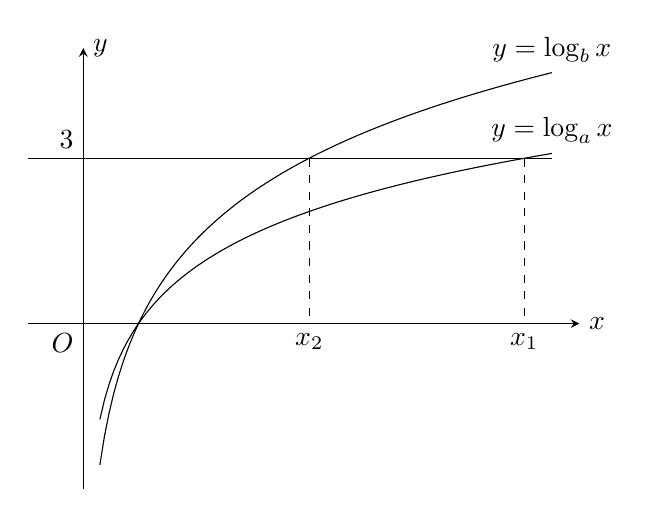
\begin{tikzpicture}[>=stealth, scale=0.7]
            \draw[->] (-1,0) --(9,0) node[right]{$x$};
            \draw[->] (0,-3) --(0,5) node[right]{$y$};
            \draw (0,0)--(0,0) node[below left]{$O$};
            \draw (-1,3)--(0,3) node[above left]{$3$}--(8.5,3);
            \draw[dashed] (4.1,3)--(4.1,0) node[below]{$x_2$};
            \draw[dashed] (8,3)--(8,0) node[below]{$x_1$};
            \draw [samples=100, domain=0.3:8.5] plot (\x, {ln(\x)/ln(1.6)})node[above]{$y=\log_bx$};
            \draw [samples=100, domain=0.3:8.5] plot (\x, {ln(\x)/ln(2)})node[above]{$y=\log_ax$};
    \end{tikzpicture}}
    \loigiai{
        Xét phương trình hoành độ giao điểm $\log_ax=3\Leftrightarrow{x_1}=a^3$, và $\log_bx=3\Leftrightarrow{x_2}=b^3$.\\
        Ta có $x_1=2x_2\Leftrightarrow{a^3}=2b^3\Leftrightarrow{\left(\dfrac{a}{b}\right)^3}=2\Leftrightarrow\dfrac{a}{b}=\sqrt[3]{2}$.
    }
\end{ex}

\begin{ex}%[2D2B4-3]
    Tìm tập hợp tất cả các giá trị thực của tham số $ m$ để hàm số $ y=\ln \left(x^2+1\right)-mx+1$ đồng biến trên khoảng $\left(-\infty ;+\infty\right)$.
    \choice
    {$\left[1;+\infty\right)$}
    {$\left(-\infty ;-1\right)$}
    {$\left[-1;1\right]$}
    {\True $\left(-\infty ;-1\right]$}
    \loigiai{
        Ta có $y'=\dfrac{2x}{x^2+1}-m$.\\
        Hàm số $ y=\ln \left(x^2+1\right)-mx+1$ đồng biến trên khoảng $\left(-\infty ;+\infty\right)$
        $$\Leftrightarrow y'\ge 0,\forall x\in\left(-\infty ;+\infty\right)\Leftrightarrow  g(x)=\dfrac{2x}{x^2+1}\ge m,\forall x\in\left(-\infty ;+\infty\right).$$
        Ta có $g'(x)=\dfrac{-2x^2+2}{\left(x^2+1\right)^2}=0\Leftrightarrow x=\pm 1$\\
        Bảng biến thiên
        \begin{center}
            
\begin{tikzpicture}
                \tkzTabInit[nocadre,lgt=1.2,espcl=3]{$x$/0.8,$g'(x)$/0.8,$g(x)$/2.5}{$-\infty$,$-1$,$1$,$+\infty$}
                \tkzTabLine{,-,0,+,0,-,}
                \tkzTabVar{+/$0$,-/$-1$,+/$1$,-/$0$}
            \end{tikzpicture}
        \end{center}
        Dựa vào bảng biến thiên ta có: $ g(x)=\dfrac{2x}{x^2+1}\ge m,\forall x\in\left(-\infty ;+\infty\right)\Leftrightarrow  m\le-1$.
    }
\end{ex}

\begin{ex}%[2D2B4-3]
    [Chuyên ĐHSP Hà Nội 2019]%Câu 29
    \immini{Trong hình dưới đây, điểm $ B$ là trung điểm của đoạn thẳng $ AC$. Khẳng định nào sau đây là đúng?	\choice
        {$ a+c=2b$}
        {\True $ ac=b^2$}
        {$ ac=2b^2$}
        {$ ac=b$}}
    {\begin{tikzpicture}[>=stealth, scale=0.7]
            \draw[->] (-1,0) --(7,0) node[right]{$x$};
            \draw[->] (0,-2) --(0,3) node[right]{$y$};
            \draw (0,0)--(0,0) node[below left]{$O$};
            \draw[dashed] (0,0.6)node[left]{$A$}--(1.82,0.6)--(1.82,0) node[below]{$a$};
            \draw[dashed] (0,1.2)node[left]{$B$}--(3.32,1.2)--(3.32,0) node[below]{$b$};
            \draw[dashed] (0,1.8)node[left]{$C$}--(6.05,1.8)--(6.05,0) node[below]{$c$};
            %	\draw (-1,0.1)--(-1,-0.1) node[above]{$-1$};
            \draw [samples=100, domain=0.3:7] plot (\x, {ln(\x)})node[above]{$y=\ln x$};
        \end{tikzpicture}
    }
    \loigiai{
        Ta có $ A\left(0;\ln a\right)$, $ B\left(0;\ln b\right)$, $ C\left(0;\ln c\right)$ và $ B$ là trung điểm của $ AC$ nên
        $$\ln a+\ln c=2\ln b\Leftrightarrow\ln \left(ac\right)=\ln {b^2}\Leftrightarrow ac=b^2.$$
        Vậy $ ac=b^2$.
    }
\end{ex}
\begin{ex}%[2D2B4-3]
    Cho các số thực $a,b$ sao cho $0<a$, $b\ne 1$, biết rằng đồ thị các hàm số $y=a^x$ và $y=\log_bx$ cắt nhau tại điểm $ M\left(\sqrt{2018};\sqrt[5]{2019^{-1}}\right)$. Mệnh đề nào dưới đây đúng?
    \choice
    {$a>1,b>1$}
    {$a>1,0<b<1$}
    {\True $0<a<1,b>1$}
    {$0<a<1,0<b<1$}
    \loigiai{
        Vì $ M\left(\sqrt{2018};\sqrt[5]{2019^{-1}}\right)$ thuộc đồ thị hàm số $y=a^x$ nên ta có
        $$a^{\sqrt{2018}}=\sqrt[5]{2019^{-1}}=\dfrac{1}{\sqrt[5]{2019}}<1=a^0\Rightarrow 0<a<1.$$
        Vì $ M\left(\sqrt{2018};\sqrt[5]{2019^{-1}}\right)$ thuộc đồ thị hàm số $y=\log_bx$ nên ta có
        $$\log_b\sqrt{2018}=\sqrt[5]{2019^{-1}}\Rightarrow{b^{\tfrac{1}{\sqrt[5]{2019}}}}=\sqrt{2018}>1=b^0\Rightarrow b>1.$$
        Vậy $0<a<1$, $b>1$.
    }
\end{ex}
\begin{ex}%[2D2B4-3]
    [Sở Hà Nội 2019]
    Tập tất cả các giá trị của tham số $ m$ để hàm số $ y=\ln \left(x^2+1\right)-mx+1$ đồng biến trên $\mathbb{R}$ là
    \choice
    {$\left[-1;1\right]$}
    {$\left(-\infty ;-1\right)$}
    {$\left(-1;1\right)$}
    {\True $\left(-\infty ;-1\right]$}
    \loigiai{
        Tập xác định $\mathscr{D}=\mathbb{R}$.\\
        Ta có $y'=\dfrac{2x}{x^2+1}-m=\dfrac{-m{x^2}+2x-m}{x^2+1}$\\
        Để hàm số đồng biến trên $\mathbb{R}$ điều kiện là
        $$y'\ge 0,\forall x\in\mathbb{R}\Leftrightarrow-m{x^2}+2x-m\ge 0,\forall x\in\mathbb{R}\Leftrightarrow\heva{&-m>0\\&\Delta'=1-m^2\le 0}\Leftrightarrow m\in\left(-\infty; -1\right].$$
    }
\end{ex}
\begin{ex}%[2D2B4-3]
    [THPT Đông Sơn Thanh Hóa 2019]
    \immini
    {
        Trong hình vẽ bên có đồ thị các hàm số $ y=a^x$, $y=b^x$, $y=\log_cx$. Hãy chọn mệnh đề đúng trong các mệnh đề sau đây?
        \choice
        {\True $ a<c<b$}
        {$ c<a<b$}
        {$ a<b=c$}
        {$ b<c<a$}
    }
    {
        \begin{tikzpicture}[>=stealth, scale=1,scale=.7]
            \draw[->] (-3,0) -- (0,0) node[below left]{$O$} -- (6,0) node[below]{$x$};
            \draw[->] (0,-2) -- (0,0) -- (0,6) node[below right]{$y$};
            \draw[ samples=200,domain=-3:2.5] plot(\x,{(0.6)^(\x)})node[right]{$y=a^x$};
            \draw[ samples=200,domain=-3:1.5] plot(\x,{(3)^(\x)})node[right]{$y=b^x$};
            \draw[smooth,samples=100] plot[domain=0.7:4.2] (\x,{ln(\x)/ln(1.3)}) node[right]{$y=\log_cx$};
        \end{tikzpicture}
    }
    \loigiai{
        Dựa vào đồ thị các hàm số $ y=a^x$, $y=b^x$, $y=\log_cx$, ta có\\
        Hàm số $ y=a^x$ nghịch biến trên $\mathbb{R}$ nên ta có $ 0<a<1$ \hfill{$(1)$}\\
        Các hàm số $ y=b^x$, $y=\log_cx$ đồng biến trên tập xác định của nó nên ta có $\heva{&b>1\\& c>1}$ \hfill{$(2)$}\\
        Từ $(1)$, $(2)\Rightarrow\heva{&a<b\\ & a<c.}$\\
        Nếu $b=c$ thì ta có đồ thị hai hàm số ! đối xứng nhau qua đường thẳng $y=x$.\\
        Tuy nhiên nhìn hình dáng hai đồ thị hàm số $y=b^x$, $y=\log_bx$ không có tính chất đối xứng nhau qua đường thẳng $y=x$.\\
        Vậy $a<c<b$.
    }
\end{ex}
\begin{ex}%[2D2B4-3]
    [Lương Thế Vinh Hà Nội 2019]%Câu 33
    \immini{
        Cho đồ thị của ba hàm số $y=a^x$, $y=b^x$, $y=c^x$ như hình vẽ bên. Khẳng định nào sau đây đúng?
        \choice
        {$b>a>c$}
        {$a>c>b$}
        {\True $c>a>b$}
        {$c>b>a$}
    }{
        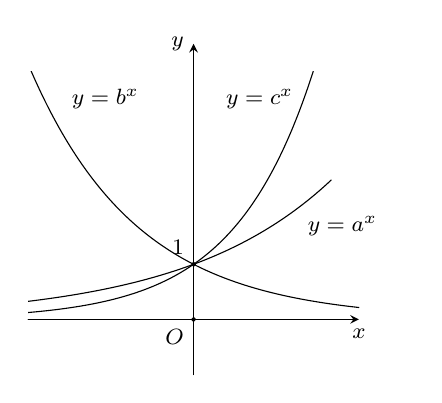
\begin{tikzpicture}[>=stealth,scale=0.7, line join = round, line cap = round, font=\footnotesize]
            \tikzset{label style/.style={font=\footnotesize}}
            \draw[->](-3,0)--(3,0) node[below]{$x$};
            \draw[->](0,-1)--(0,5) node[left]{$y$};
            \clip (-3,-1) rectangle (4,4.5);
            \draw[smooth, samples=300,domain=-3:2.5]
            plot (\x,{2^(\x)});
            \draw[smooth, samples=300,domain=-3:2.5]
            plot (\x,{1.45^(\x)});
            \draw[smooth, samples=300,domain=-3:3]
            plot (\x,{0.6^(\x)});
            \draw [fill=black](0,0) node[below left]{$O$} circle(1pt);
            \draw [fill=black](0,1) node[above left]{$1$} circle(1pt);
            \draw (-1.6,4) node[]{$y=b^x$};
            \draw (1.2,4) node[]{$y=c^x$};
            \draw (2.7,1.7) node[]{$y=a^x$};
        \end{tikzpicture}
    }
    \loigiai{
        \immini{
            Kẻ đường thẳng $x=1$, đường thẳng này cắt đồ thị $y=b^x$, $y=a^x$, $y=c^x$ lần lượt tại các điểm có tung độ $b$, $a$, $c$.\\
            Dựa vào đồ thị ta có $b<a<c$.
        }{
            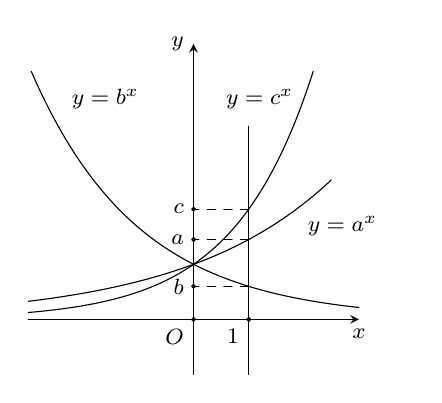
\begin{tikzpicture}[>=stealth,scale=0.7, line join = round, line cap = round,font=\footnotesize]
                \tikzset{label style/.style={font=\footnotesize}}
                \draw[->](-3,0)--(3,0) node[below]{$x$};
                \draw[->](0,-1)--(0,5) node[left]{$y$};
                \clip (-3,-1) rectangle (4,4.5);
                \draw[smooth, samples=300,domain=-3:2.5]
                plot (\x,{2^(\x)});
                \draw[smooth, samples=300,domain=-3:2.5]
                plot (\x,{1.45^(\x)});
                \draw[smooth, samples=300,domain=-3:3]
                plot (\x,{0.6^(\x)});
                \draw[fill=black] (0,0) node[below left]{$O$} circle(1pt);
                \draw[fill=black] (1,0) node[below left]{$1$} circle(1pt);
                \draw (-1.6,4) node[]{$y=b^x$};
                \draw (1.2,4) node[]{$y=c^x$};
                \draw (2.7,1.7) node[]{$y=a^x$};
                \draw (1,-1)--(1,3.5);
                \draw[dashed] (1,0.6)--(0,0.6) (1,1.45)--(0,1.45) (1,2)--(0,2);
                \draw [fill=black](0,0.6) node[left]{$b$} circle(1pt) (0,1.45) node[left]{$a$} circle(1pt) (0,2) node[left]{$c$} circle(1pt);
            \end{tikzpicture}
        }
    }
\end{ex}
\begin{ex}%[2D2B4-3]
    [KTNL GV THPT Lý Thái Tổ 2019]
    \immini{
        Cho $a$, $b$, $c$ là các số thực dương khác $1$. Hình vẽ bên là đồ thị của hàm số $y=\log_a x$, $y=\log_b x$, $y=\log_c x$.
        Khẳng định nào sau đây đúng?
        \choice
        {$c<b<a$}
        {\True $c<a<b$}
        {$a<c<b$}
        {$a<b<c$}
    }{
        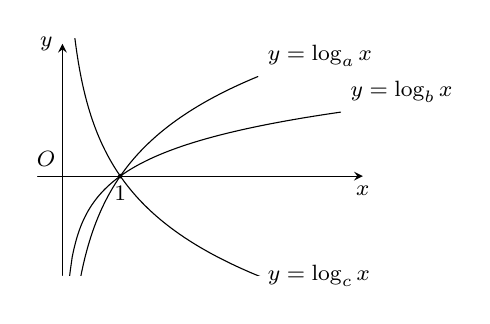
\begin{tikzpicture}[scale=0.7,>=stealth, font=\footnotesize, line join=round, line cap=round]
            \draw[-> ] (-0.5,0) -- (5.4,0)node[below] {$x$};
            \draw[-> ] (-0.05,-1.8) -- (-0.05,2.4)node[left] {$y$};
            \draw(0,0) node[above left] { $O$};
            \draw[fill = black] (3.5,-1.808) node [right]{$ y = \log_c x $} ;
            \draw[fill = black] (5,1.16) node [above right]{$ y = \log_b x $} ;
            \draw[fill = black] (3.5,1.808) node [above right]{$ y = \log_a x $} ;
            \clip (-0.5,-1.8) rectangle (5.4,2.5);
            \draw[samples=300,domain=0.01:3.5] plot(\x,{ (ln(\x )/ln(2))  });
            \draw[samples=300,domain=0.01:5] plot(\x,{ (ln(\x )/ln(4))  });
            \draw[samples=300,domain=0.01:5] plot(\x,{ (ln(\x )/ln(0.5))  });
            \draw[fill = black](1,0) node[below]{$ 1 $} circle(1pt);
        \end{tikzpicture}
    }
    \loigiai{
        \immini{
            Kẻ đường thẳng $ y = 1 $ cắt đồ thị hàm số $ y = \log_a x $, $ y = \log_b x $ và $ y = \log_c x $ lần lượt tại $ A $, $ B $ và $ C $.	\\
            Từ đồ thị, ta thấy $ c < a < b $.
        }{
            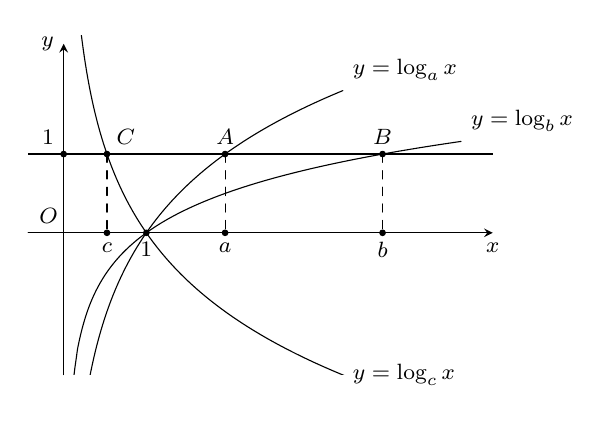
\begin{tikzpicture}[line cap=round,line join=round,x=1.0cm,y=1.0cm,>=stealth,scale=1, font = \footnotesize]
                \draw[-> ] (-0.5,0) -- (5.4,0)node[below] {$x$};
                \draw[-> ] (-0.05,-1.8) -- (-0.05,2.4)node[left] {$y$};
                \draw(0,0) node[above left] { $O$};
                \draw[fill = black] (3.5,-1.808) node [right]{$ y = \log_c x $} ;
                \draw[fill = black] (5,1.16) node [above right]{$ y = \log_b x $} ;
                \draw[fill = black] (3.5,1.808) node [above right]{$ y = \log_a x $} ;
                \clip (-0.5,-1.8) rectangle (5.4,2.5);
                \draw[samples=300,domain=0.01:3.5] plot(\x,{ (ln(\x )/ln(2))  });
                \draw[samples=300,domain=0.01:5] plot(\x,{ (ln(\x )/ln(4))  });
                \draw[samples=300,domain=0.01:5] plot(\x,{ (ln(\x )/ln(0.5))  });
                \draw(-0.5,1)--(5.4,1);
                \draw[dashed](2,1)--(2,0) (4,1)--(4,0) (0.5,1)--(0.5,0);
                \draw[fill = black](2,0) node[below]{$ a $} circle(1pt);
                \draw[fill = black](4,0) node[below]{$ b $} circle(1pt);
                \draw[fill = black](4,1) node[above]{$ B $} circle(1pt);
                \draw[fill = black](2,1) node[above]{$ A $} circle(1pt);
                \draw[fill = black](0.5,1) node[above right]{$ C $} circle(1pt);
                \draw[fill = black](0.5,0) node[below]{$ c $} circle(1pt);
                \draw[fill = black](-0.05,1) node[above left]{$ 1 $} circle(1pt);
                \draw[fill = black](1,0) node[below]{$ 1 $} circle(1pt);
            \end{tikzpicture}
        }
    }
\end{ex}
\begin{ex}%[2D2B4-3]
    [Chuyên Thái Bình 2019]
    \immini
    {
        Cho $ a$, $b$, $c$ là các số thực dương khác $1$. Hình vẽ bên là đồ thị hàm số $ y=\log_ax$, $y=y=\log_bx$, $y=\log_cx$. Khẳng định nào sau đây là đúng?
        \choice
        {\True $a<b<c$}
        {$ a<c<b$}
        {$ b<a<c$}
        {$ b>a>c$}
    }
    {
        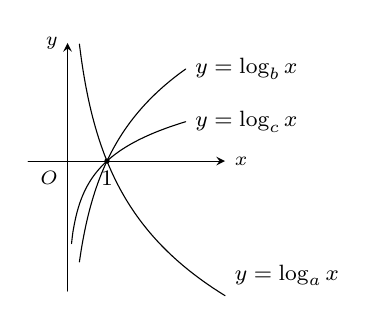
\begin{tikzpicture}[scale=0.5, font=\footnotesize,
            line join=round, line cap=round, >=stealth]
            \def\a{1/1.5}
            \def\b{1.6}
            \def\c{3}
            \draw[->] (-1,0) -- (4,0) node[right] {\scriptsize $x$};
            \draw[->] (0,-3.3) -- (0,3) node[left] {\scriptsize $y$};
            \draw (0,0)node[below left]{\scriptsize $O$};
            \draw[fill=black]  (1,0) node[below]{$1$} circle (1.5pt);
            \draw[,samples=100,smooth,domain=0.3:4] plot(\x,{ln(\x)/ln(\a)})node[above right]{$y=\log_a x$};
            \draw[,samples=100,smooth,domain=0.3:3] plot(\x,{ln(\x)/ln(\b)})node[right]{$y=\log_b x$};
            \draw[,samples=100,smooth,domain=0.1:3] plot(\x,{ln(\x)/ln(\c)})node[right]{$y=\log_c x$};
        \end{tikzpicture}
    }
    \loigiai{
        Do $ y=\log_bx$ và $ y=\log_cx$ là hai hàm đồng biến nên $ b$, $c>1$.\\
        Do $ y=\log_ax$ nghịch biến nên $ 0<a<1$.\\
        Mặt khác lấy $ y=m$, khi đó tồn tại $x_1$, ${x_2}>0$ để $\heva{&{\log_b}{x_1}=m\\&{\log_c}{x_2}=m}\Rightarrow\heva{&{b^m}=x_1\\&{c^m}=x_2.}$\\
        Dễ thấy $x_1<x_2\Rightarrow{b^m}<c^m\Rightarrow b<c$.\\
        Vậy $ a<b<c$.
    }
\end{ex}
\begin{ex}%[2D2K4-3]
    [THPT Nguyễn Khuyến 2019]
    Cho hàm số $y=\dfrac{\ln x-6}{\ln x-2m}$ với $m$ là tham số. Gọi $S$ là tập hợp các giá trị nguyên dương của $m$ để hàm số đồng biến trên khoảng $\left(1;e\right)$. Tìm số phần tử của $S$.
    \choice
    {$ 3$}
    {$ 1$}
    {\True $ 2$}
    {$ 4$}
    \loigiai{
        Điều kiện $\ln x\ne 2m\Leftrightarrow x\ne{{e}^{2m}}$.\\
        Có $y'=\dfrac{6-2m}{x{\left(\ln x-2m\right)^2}}$\\
        Hàm số đồng biến trên $\left(1;e\right)\Leftrightarrow y'>0, \forall x\in\left(1;e\right)\Leftrightarrow\dfrac{6-2m}{x{\left(\ln x-2m\right)^2}}>0, \forall x\in\left(1;e\right)$\\
        $\Leftrightarrow \heva{& 6-2m>0\\&e^{2m}\notin\left(1;e\right)} \Leftrightarrow\heva{& 6-2m>0\\& \hoac{&{{e}^{2m}}\le 1\\& {{e}^{2m}}\ge{e}}} \Leftrightarrow\heva{& m<3\\& \hoac{& m\le 0\\&  m\ge\dfrac{1}{2}}} \Leftrightarrow\hoac{& m\le 0\\& \dfrac{1}{2}\le m<3.}$\\
        Do $m$ nguyên dương nên $m\in\left\{ 1;2\right\}$.\\
        Vậy tập $S$ có $2$ phần tử.
    }
\end{ex}
\begin{ex}%[2D2K4-3]
    Tìm tất cả các giá trị thực của tham số m để hàm số $ y=\dfrac{m{\log_2}x-2}{\log_2x-m-1}$ nghịch biến trên $\left(4;+\infty\right)$
    \choice
    {$ m<-2$ hoặc $ m>1$}
    {$ m\le-2$ hoặc $ m=1$}
    {$ m<-2$ hoặc $ m=1$}
    {\True $ m<-2$}
    \loigiai{
        Đặt $ t=\log_2x$.\\
        Ta có $ x\in\left(4;+\infty\right)\Leftrightarrow t\in\left(2;+\infty\right)$.\\
        Hàm số được viết lại $ y=\dfrac{mt-2}{t-m-1}$ $(1)$.\\
        Vì $ t=\log_2x$ đồng biến trên $\left(0;+\infty\right)$ nên yêu cầu bài toán $\Leftrightarrow $ $(1)$ nghịch biến trên $\left(2;+\infty\right)$\\
        $\Leftrightarrow \heva{&-m\left(m+1\right)+2<0\\&  m+1\le 2} \Leftrightarrow\heva{&\hoac{& m<-2\\&  m>1}\\&  m\le 1}\Leftrightarrow m<-2$.
    }
\end{ex}
\begin{ex}%[2D2K4-3]
    [HSG Bắc Ninh 2019]
    Cho hàm số $ y=\log_{2018}\left(\dfrac{1}{x}\right)$ có đồ thị $\left(C_1\right)$ và hàm số $ y=f(x)$ có đồ thị $\left(C_2\right)$. Biết $\left(C_1\right)$ và $\left(C_2\right)$ đối xứng nhanh qua gốc tọa độ. Hỏi hàm số $y=\left| f(x)\right|$ nghịch biến trên khoảng nào dưới đây?
    \choice
    {$\left(0;1\right)$}
    {$\left(-1;0\right)$}
    {\True $\left(-\infty;-1\right)$}
    {$\left(1;+\infty\right)$}
    \loigiai{
        Ta có $ y=\log_{2018}\left(\dfrac{1}{x}\right)$ thì $y'=-\dfrac{1}{x^2}\dfrac{1}{x\ln 2018}<0$ hàm số nghịch biến ta vẽ được đồ thị hàm số $\left(C_1\right)$ như hình
        \begin{center}
            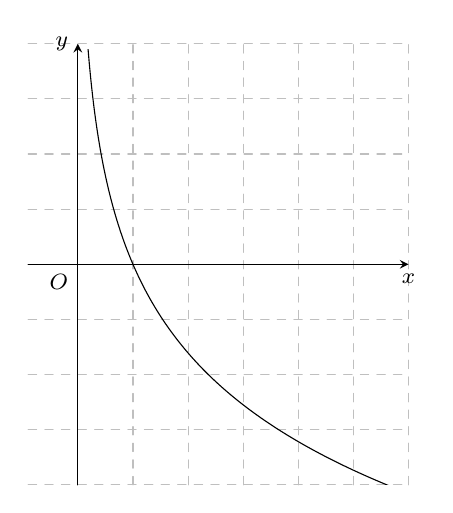
\begin{tikzpicture}[scale=.7,>=stealth, font=\footnotesize, line join=round, line cap=round]
                \def\xmax{6} \def\ymin{-4} \def\ymax{4}
                \draw[color=gray!50,dashed] (-0.9,\ymin) grid (\xmax,\ymax);
                \draw[->] (-0.9,0)--(\xmax,0) node [below]{$x$};
                \draw[->] (0,\ymin)--(0,\ymax) node [left]{$y$};
                \node at (0,0) [below left]{$O$};
                \clip (-0.9,\ymin) rectangle (\xmax-0.1,\ymax-0.1);
                \draw[smooth,samples=300,domain=0.03:\xmax] plot(\x,{ln(\x)/ln(0.65)});
            \end{tikzpicture}
        \end{center}
        Do $\left(C_2\right)$ đối xứng với $\left(C_1\right)$ qua $ O$ nên có dạng như hình dưới
        \begin{center}
            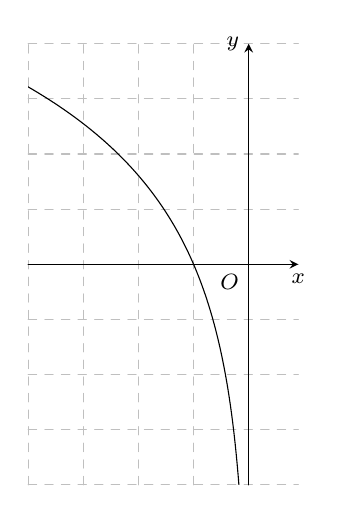
\begin{tikzpicture}[scale=.7,>=stealth, font=\footnotesize, line join=round, line cap=round]
                \def\xmax{6} \def\ymin{-4} \def\ymax{4}
                \draw[color=gray!50,dashed] (-4,\ymin) grid (.9,\ymax);
                \draw[->] (-4,0)--(.9,0) node [below]{$x$};
                \draw[->] (0,\ymin)--(0,\ymax) node [left]{$y$};
                \node at (0,0) [below left]{$O$};
                \clip (-4,\ymin) rectangle (1,\ymax-0.1);
                \draw[smooth,samples=300,domain=0.03:\xmax] plot(-\x,{-ln(\x)/ln(0.65)});
            \end{tikzpicture}
        \end{center}
        Từ đó đồ thị hàm số $ y=\left| f(x)\right|$ là
        \begin{center}
            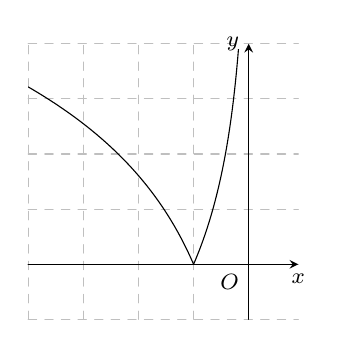
\begin{tikzpicture}[scale=.7,>=stealth, font=\footnotesize, line join=round, line cap=round]
                \def\xmax{6} \def\ymin{-1} \def\ymax{4}
                \draw[color=gray!50,dashed] (-4,\ymin) grid (.9,\ymax);
                \draw[->] (-4,0)--(.9,0) node [below]{$x$};
                \draw[->] (0,\ymin)--(0,\ymax) node [left]{$y$};
                \node at (0,0) [below left]{$O$};
                \clip (-4,\ymin) rectangle (1,\ymax-0.1);
                \draw[smooth,samples=300,domain=0.03:1] plot(-\x,{ln(\x)/ln(0.65)});
                \draw[smooth,samples=300,domain=4:1] plot(-\x,{-ln(\x)/ln(0.65)});
            \end{tikzpicture}
        \end{center}
        Dựa vào đồ thị trên ta có hàm số $ y=\left|f(x)\right|$ nghịch biến trên khoảng $\left(-\infty;-1\right)$.
    }
\end{ex}
\begin{ex}%[2D2K4-3]
    [THPT Bạch Đằng Quảng Ninh 2019]%Câu 39
    Có bao nhiêu giá trị nguyên của tham số $m \in[-2019;2019]$ để hàm số $y=\dfrac{\ln x-6}{\ln x-3m}$ đồng biến trên khoảng $\left(1;e^6\right)$?
    \choice
    {\True $2020$}
    {$2021$}
    {$2018$}
    {$2019$}
    \loigiai{
        Đặt $t=\ln x$.\\
        Khi đó hàm số $y=\dfrac{\ln x-6}{\ln x-3 m}$ đồng biến trên khoảng $\left(1 ; e^6\right)$ thì hàm số $y(t)=\dfrac{t-6}{t-3 m}$ đồng biến trên khoảng $(0 ; 6)$.\\
        Ta có $y'(t)=\dfrac{-3 m+6}{(t-3 m)^2}$\\
        Để hàm số $y(t)$ đồng biến trên khoảng $(0 ; 6)$ thì\\
        $\heva{&- 3 m + 6 > 0 \\& 3m \notin ( 0; 6 ) }\Rightarrow \heva{&m<2 \\& \hoac{&m \leq 0 \\& m \geq 2}} \Rightarrow m \leq 0 \dfrac{m \in \mathbb{Z}}{m \in[-201; 2019]} m \in\{-2019;-2018;\ldots;-1; 0\}$.\\
        Vậy có tất cả $2020$ số nguyên $m$ thoả mãn yêu cầu bài toán.
    }
\end{ex}
\begin{ex}%[2D2K4-3]
    [Chuyên Hưng Yên 2019]%Câu 40
    Có bao nhiêu giá trị nguyên của tham số thực $m$ thuộc đoạn $\left[-2018;2018\right]$ để hàm số $y=f(x)=\left(x+1\right)\ln x+\left(2-m\right)x$ đồng biến trên khoảng $\left(0;\mathrm{e}^2\right)$.
    \choice
    {$2016$}
    {$2022$}
    {$2014$}
    {\True $2023$}
    \loigiai{
        Ta có $y'=f'(x)=\ln x+\dfrac{x+1}{x}+2-m$\\
        Yêu cầu bài toán $\Leftrightarrow{f}'(x)=\ln x+\dfrac{1}{x}+3-m\ge 0\Leftrightarrow\ln x+\dfrac{1}{x}+3\ge m$; $\forall x\in\left(0;\mathrm{e}^2\right)$.\\
        Xét hàm số $g(x)=\ln x+\dfrac{1}{x}+3$ với $x\in\left(0;\mathrm{e}^2\right)$.\\
        Ta có $g'(x)=\dfrac{1}{x}-\dfrac{1}{x^2}=0\Leftrightarrow x=1$.\\
        Bảng biến thiên
        \begin{center}
            
\begin{tikzpicture}
                \tkzTabInit[nocadre,lgt=1.2,espcl=3]{$x$/0.8,$g'(x)$/0.8,$g(x)$/2.5}{$0$,$1$,$\mathrm{e}^2$}
                \tkzTabLine{,-,0,+,}
                \tkzTabVar{+/$\lim\limits_{x\to 0^+}g(x)$,-/$4$,+/$5+\dfrac{1}{\mathrm{e}^2}$}
            \end{tikzpicture}
        \end{center}
        Dựa vào bảng biến thiên suy ra $g(x)\ge 4$ với mọi $x\in\left(0;\mathrm{e}^2\right)$.\\
        Từ đó suy ra $-2018\le m\le 4$.\\
        Vậy có $ 2023$ giá trị của $ m$ thỏa mãn.
    }
\end{ex}
\begin{ex}%[2D2B4-3]
    [THPT Quang Trung Đống Đa Hà Nội 2019]%Câu 41
    Cho $f(x)=a\ln \left(x+\sqrt{x^2+1}\right)+b\sin x+6$ với $a$, $b\in\mathbb{R}$. Biết rằng $ f\left(\log\left(\log e\right)\right)=2$. Tính giá trị của $ f\left(\log\left(\ln 10\right)\right)$.
    \choice
    {\True $10$}
    {$2$}
    {$4$}
    {$8$}
    \loigiai{
        Ta có $\log\left(\log{\mathrm{e}}\right)+\log\left(\ln 10\right)=\log 1=0$.\\
        Mặt khác $f(x)+f\left(-x\right)=a\ln \left(x+\sqrt{x^2+1}\right)+b\sin x+6+a\ln \left(-x+\sqrt{x^2+1}\right)+b\sin\left(-x\right)+6$\\
        $=a\ln \left(x+\sqrt{x^2+1}\right)\left(-x+\sqrt{x^2+1}\right)+b\sin x-b\sin x+12$\\
        $=a\ln 1+12=12\forall x\in\mathbb{R}$.\\
        Khi đó suy ra $ f\left(\log\left(\log{\mathrm{e}}\right)\right)+f\left(\log\left(\ln 10\right)\right)=12$ $\Rightarrow  f\left(\log\left(\ln 10\right)\right)=10$.
    }
\end{ex}
\begin{ex}%[2D2B4-3]
    [Sở Bắc Ninh 2019]%Câu 42
    \immini
    {
        Cho $a$, $b$, $c$ dương và khác $1$. Đồ thị các hàm số $y=\log_ax$, $y=\log_bx$, $y=\log_cx$ như hình vẽ.\\
        Khẳng định nào dưới đây đúng?
        \choice
        {\True $a>c>b$}
        {$a>b>c$}
        {$c>b>a$}
        {$b>c>a$}
    }
    {
        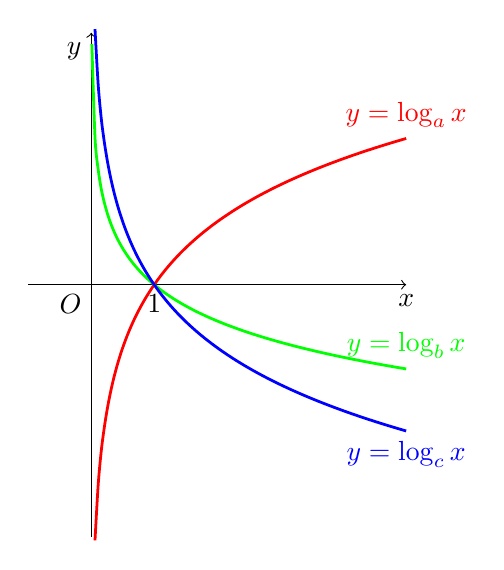
\begin{tikzpicture}[scale=.8]
            \draw[->] (-1,0)--(0,0) node[below left]{$O$}--(5,0) node[below]{$x$};
            \draw[->] (0,-4)--(0,4) node[below left]{$y$};
            \draw[smooth, red, line width=1,samples=100] plot[domain=0.06:5] (\x,{log2(\x)}) node[above]{$y=\log_ax$};
            \draw[smooth, green, line width=1,samples=100] plot[domain=0.01:5] (\x,{ln(\x)/ln(0.3)}) node[above]{$y=\log_bx$};
            \draw[smooth, blue, line width=1,samples=100] plot[domain=0.06:5] (\x,{ln(\x)/ln(0.5)}) node[below]{$y=\log_cx$};
            \draw[dashed] (1,0) node[below]{$1$};
        \end{tikzpicture}
    }
    \loigiai{
        Dựa vào đồ thị ta thấy đồ thị hàm số $y=\log_ax$ đồng biến trên tập xác định nên $a>1$.\\
        Đồ thị hàm số $y=\log_bx$ và $y=\log_cx$ nghịch biến trên tập xác định nên $0<b<1$, $0<c<1$.\\
        Suy ra $a>b$ và $a>c$.\\
        Mặt khác với $x>1$ ta có $\log_bx>\log_cx\Rightarrow b<c$.\\
        Vậy $a>c>b$.
    }
\end{ex}
\begin{ex}%[2D2B4-3]
    Đồ thị hàm số $y=f(x)$ đối xứng với đồ thị hàm số $y=a^x$, $\left(a>0,a\ne 1\right)$ qua điểm $I(1;1)$. Giá trị của biểu thức $f\left(2+\log_a\dfrac{1}{2018}\right)$ bằng
    \choice
    {$2016$}
    {\True $-2016$}
    {$2020$}
    {$-2020$}
    \loigiai{
        Gọi $(C)$ là đồ thị hàm số $y=a^x$; $\left(C_1\right)$ là đồ thị hàm số $y=f(x)$.\\
        $M\left(2+\log_a\dfrac{1}{2018};{y_M}\right)\in\left(C_1\right)$ $\Leftrightarrow{y_M}=f\left(2+\log_a\dfrac{1}{2018}\right)$.\\
        Gọi $N$ đối xứng với $M$ qua $I\left(1;1\right)$ $\Rightarrow N\left(-\log_a\dfrac{1}{2018};2-y_M\right)$.\\
        Do đồ thị $\left(C_1\right)$ đối xứng $(C)$ qua $I\left(1;1\right)$ nên $N\left(-\log_a\dfrac{1}{2018};2-y_M\right)\in(C)$.\\
        $N\in(C)$ $\Leftrightarrow 2-y_M=a^{-\log_a\dfrac{1}{2018}}$ $\Leftrightarrow 2-y_M=a^{\log_a2018}$ $\Leftrightarrow 2-y_M=2018$ $\Leftrightarrow{y_M}=-2016$.\\
        Vậy $f\left(2+\log_a\dfrac{1}{2018}\right)=-2016$.
    }
\end{ex}
\begin{ex}%[2D2K4-3]
    [Chuyên Hùng Vương - Phú Thọ - 2020]%Câu 44
    \immini
    {
        Trong hình vẽ bên các đường cong $\left({C}_1\right)\colon y=a^x$, $\left({C}_2\right)\colon y=b^x$, $\left({C}_3\right)\colon y=c^x$ và đường thẳng $y=4$; $y=8$ tạo thành hình vuông $MNPQ$ có cạnh bằng $4$.\\
        Biết rằng $abc=2^{\frac{x}{y}}$ với $x;y\in{\mathbb{Z}^+}$ và $\dfrac{x}{y}$ tối giản, giá trị của $x+y$ bằng
        \choice
        {$ 34$}
        {$ 5$}
        {\True $ 43$}
        {$ 19$}
    }
    {
        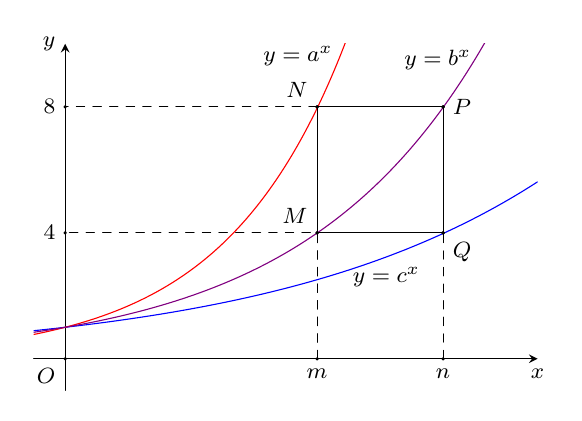
\begin{tikzpicture}[scale=0.4, font=\footnotesize, line join=round, line cap=round, >=stealth]
            \draw[->] (-1,0)--(15,0) node[below] {$x$};
            \draw[->] (0,-1)--(0,10) node[left] {$y$};
            \draw[fill=black] (0,0) circle(1pt) node[below left] {$O$};
            \draw[fill=black] (0,8) circle(1pt) node[left] {$8$};
            \draw[fill=black] (0,4) circle(1pt) node[left] {$4$};
            \draw[fill=black] (8,0) circle(1pt) node[below] {$m$};
            \draw[fill=black] (12,0) circle(1pt) node[below] {$n$};

            \draw (8.8,9.6) node[left]{$y=a^x$};
            \draw (13.2,9.5) node[left]{$y=b^x$};
            \draw (10.2,3.2) node[below]{$y=c^x$};
            \clip (-1,-1) rectangle (15,10);
            \draw[color=blue,samples=100,smooth,domain=-1:15] plot(\x,{(1.122)^(\x)});
            \draw[color=red,samples=100,smooth,domain=-1:15] plot(\x,{(1.296)^(\x)});
            \draw[color=violet,samples=100,smooth,domain=-1:15] plot(\x,{(1.189)^(\x)});
            \draw (8,4)--(12,4)--(12,8)--(8,8)--(8,4);
            \draw[dashed] (8,0)--(8,4)--(0,4);
            \draw [dashed] (8,0)--(8,4) (12,0)--(12,4) (8,8)--(0,8);
            \draw (8,8) circle (1.2pt) node[above left]{$N$};
            \draw (8,4) circle (1.2pt) node[above left]{$M$};
            \draw (12,8) circle (1.2pt) node[right]{$P$};
            \draw (12,4) circle (1.2pt) node[below right]{$Q$};
        \end{tikzpicture}
    }
    \loigiai{
        Giả sử hoành độ điểm $ M$ là $ m$, ta suy ra $ M\left(m;4\right){;}N\left(m;8\right);P\left(m+4;8\right){; Q}\left(m+4;4\right)$.\\
        Từ giả thiết ta có $ M,P$ thuộc đường cong $ y=b^x$ nên $\heva{&{b^m}=4\\& {b^{m+4}}=8}\Leftrightarrow\heva{&{b^m}=4\\& {b^4}=2}\Leftrightarrow\heva{& m=8\\&  b=2^{\tfrac{1}{4}}.}$\\
        $ N$, $Q$ lần lượt thuộc đường cong $ y=a^x$; $y=c^x$ nên $\heva{&{a^8}=8\\& {c^{12}}=4}\Leftrightarrow\heva{&{a^8}=2^3\\& {c^{12}}=2^2}\Leftrightarrow\heva{& a=2^{\tfrac{3}{8}}\\&  c=2^{\tfrac{1}{6}}.}$\\
        Khi đó $abc=2^{\frac{3}{8}}{2^{\frac{1}{4}}}{2^{\frac{1}{6}}}=2^{\frac{3}{8}+\frac{1}{4}+\frac{1}{6}}=2^{\frac{19}{24}}$.\\
        Vậy $ x=19$; $y=24\Rightarrow x+y=43$.
    }
\end{ex}
\begin{ex}%[2D2B4-3]
    [Bạc Liêu - Ninh Bình 2019]%Câu 45
    \immini
    {
        Cho hàm số $y=f(x)$. Hàm số $y=f'(x)$ có đồ thị như hình vẽ.
        Hàm số $y=f(2+\mathrm{e}^x)$ nghịch biến trên khoảng
        \choice
        {$\left(-1 ; 3\right)$}
        {$\left(-2 ; 1\right)$}
        {\True $\left(-\infty ; 0\right)$}
        {$\left(0 ;+\infty\right)$}
    }
    {
        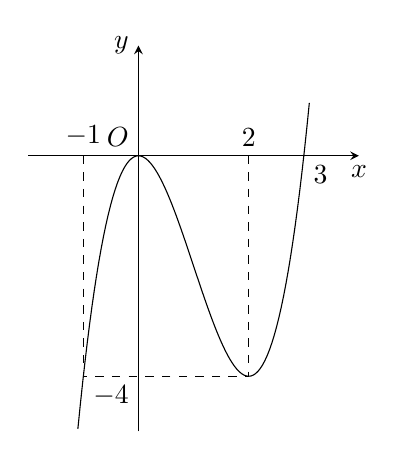
\begin{tikzpicture}[>=stealth,scale=0.7]
            \draw[->] (-2,0)--(4,0)node[below]{$x$};
            \draw[->] (0,-5)--(0,2)node[left]{$y$};
            \draw[samples=100,domain=3.1:-1.1] plot (\x,{(\x)^3-3*(\x)^2-0*(\x)});
            \draw(0,0)node[above left]{$O$};
            \draw[dashed]
            (3,0)node[below right]{$3$}
            (2,0)node[above]{$2$}
            (-1,0)node[above]{$-1$}
            (0,-4) node[below left]{$-4$}
            (2,0)--(2,-4)--(0,-4)
            (-1,0)--(-1,-4)--(0,-4)
            ;
        \end{tikzpicture}
    }
    \loigiai{
        Ta có $y'=\mathrm{e}^x f'\left(2+\mathrm{e}^x\right)$.\\
        Hàm số $y=f\left(2+e^x\right)$ nghịch biến khi và chỉ khi
        $$y'\leq 0 \Leftrightarrow \mathrm{e}^x f'\left(2+e^x\right) \leq 0 \Leftrightarrow f'(2+\mathrm{e}^x )\leq 0 \Leftrightarrow 2+e^{x}\leq 3 \Leftrightarrow \mathrm{e}^x \leq 1 \Leftrightarrow x \leq 0$$
    }
\end{ex}
\begin{ex}%[2D2K4-3]
    Có bao nhiêu giá trị nguyên của tham số $m \in[-2019 ; 2019]$ để hàm số $y=\dfrac{\ln x-6}{\ln x-3 m}$ đồng biến trên khoảng $\left(1 ; \mathrm{e}^6\right)$?
    \choice
    {\True $2020$}
    {$2021$}
    {$2018$}
    {$2019$}
    \loigiai{
        Đặt $t=\ln x$.\\
        Khi đó hàm số $y=\dfrac{\ln x-6}{\ln x-3 m}$ đồng biến trên khoảng $\left(1;\mathrm{e}^6\right)$ thì hàm số $y(t)=\dfrac{t-6}{t-3 m}$ đồng biến trên khoảng $(0;6)$.\\
        Ta có $y'(t)=\dfrac{-3 m+6}{(t-3 m)^2}$\\
        Để hàm số $y(t)$ đồng biến trên khoảng $(0 ; 6)$ thì\\
        $\heva{&{- 3 m + 6 > 0}\\& {3 m \notin ( 0; 6 )}}\Rightarrow \heva{&m<2 \\& {\hoac{&m \leq 0 \\& m \geq 2}}}\Rightarrow m \leq 0 \dfrac{m \in \mathbb{Z}}{m \in[-2019; 2019]}\Rightarrow m \in\{-2019;-2018; \ldots-1; 0\}$.\\
        Vậy có tất cả $2020$ số nguyên $m$ thoả mãn yêu cầu bài toán.
    }
\end{ex}
\begin{ex}%[2D2K4-3]
    [Chuyên Lê Hồng Phong Nam Định 2019]%Câu 47
    Cho hàm số $y=f(x)$. Đồ thị hàm số $y=f'(x)$ như hình bên dưới
    \begin{center}
        \begin{tikzpicture}[>=stealth, line join=round, line cap=round, font=\footnotesize, scale=1]
            \draw[->] (-2,0)--(5,0)node[below]{$x$};
            \draw[->] (0,-2)--(0,5) node[left]{$y$};
            \draw[samples=150,smooth,domain=-1.1:4.6] plot (\x,{0.1*(\x+1)*(\x-1)*(\x-2)*(\x-4)^2});
            \fill (-1,0) circle (1pt)node[below left]{$1$}
            (1,0) circle (1pt)node[below left]{$1$}
            (2,0) circle (1pt)node[below right]{$2$}
            (4,0) circle (1pt)node[below]{$4$}
            ;
        \end{tikzpicture}
    \end{center}
    Hàm số $g(x)=\left(\dfrac{1}{2}\right)^{f(1-2 x)}$ nghịch biến trên khoảng nào trong các khoảng sau?
    \choice
    {$(-\infty ; 0)$}
    {$(0 ; 1)$}
    {$(-1 ; 0)$}
    {\True $(1 ;+\infty)$}
    \loigiai{
        Dựa vào đồ thị, suy ra $f'(x)<0 \Leftrightarrow\hoac{&x<-1 \\& 1<x<2}$.\\
        Ta có $g'(x)=\left(\dfrac{1}{2}\right)^{f(1-2 x)}f'(1-2 x) \cdot(-2) \cdot \ln \dfrac{1}{2}$.\\
        Xét $g'(x)<0 \Leftrightarrow f'(1-2 x)<0 \Leftrightarrow\hoac{&1-2 x<-1 \\& 1<1-2 x<2}\Leftrightarrow\hoac{&x>1 \\& -\dfrac{1}{2}<x<0.}$\\
        Vậy $g(x)$ nghịch biến trên các khoảng $\left(-\dfrac{1}{2}; 0\right)$ và $(1 ;+\infty)$.
    }
\end{ex}
\begin{ex}%[2D2K4-3]
    [Kiểm tra năng lực - ĐH - Quốc Tế - 2019]%Câu 48
    Xét hàm số $f(x)=(\cos x)^{\sin x}$. Mệnh đề nào sau đây là đúng?
    \choice
    {Hàm số $f$ tăng trên khoảng $\left(0 ; \dfrac{\pi}{2}\right)$}
    {Hàm số $f$ tăng trên khoảng $\left(-\dfrac{\pi}{2}; 0\right)$}
    {\True Hàm số $f$ giảm trên khoảng $\left(-\dfrac{\pi}{2}; \dfrac{\pi}{2}\right)$}
    {$3$ lựa chọn kia đều sai}
    \loigiai{
        Nhận xét $\forall x \in\left(-\dfrac{\pi}{2}; \dfrac{\pi}{2}\right) \Rightarrow\heva{&\cos x>0 \\& f(x)>0}$.\\
        Ta có
        \allowdisplaybreaks
        $\begin{aligned}[t]
            f(x)=(\cos x)^{\sin x}\Rightarrow& \ln f(x)=\ln (\cos x)^{\sin x}=\sin x \cdot \ln (\cos x)\\
            \Rightarrow& [\ln f(x)]'=[\sin x \cdot \ln (\cos x)]'\\
            \Rightarrow& \dfrac{f'(x)}{f(x)}=\dfrac{\cos ^2 x \cdot \ln \cos x-\sin ^2 x}{\cos x}\\
            \Rightarrow& f'(x)=\dfrac{\cos ^2 x \cdot \ln \cos x-\sin ^2 x}{\cos x}\cdot f(x).
        \end{aligned}$\\
        Do $\forall x \in\left(-\dfrac{\pi}{2}; \dfrac{\pi}{2}\right) \Rightarrow \cos x \in(0 ; 1]$.\\ Mặt khác $\mathrm{e}>1 \Rightarrow \ln \cos x \leq 0$.\\
        $\Rightarrow \cos ^2 x \cdot \ln \cos x-\sin ^2 x \leq 0, \forall x \in\left(-\dfrac{\pi}{2}; \dfrac{\pi}{2}\right)$.\\
        $\Rightarrow f'(x)=\left(\dfrac{\cos ^2 x \cdot \ln \cos x-\sin ^2 x}{\cos x}\right) \cdot f(x) \leq 0, \forall x \in\left(-\dfrac{\pi}{2}; \dfrac{\pi}{2}\right)$ (dấu \lq\lq =\rq\rq\, xảy ra khi $x=0$).\\
        Vậy $y=f(x)$ giảm trên $\left(-\dfrac{\pi}{2}; \dfrac{\pi}{2}\right)$.
    }
\end{ex}
\begin{ex}%[2D2K4-3]
    Có bao nhiêu giá trị nguyên của tham số $m$ trong đoạn $[-2019 ; 2019]$ để hàm số $y=\ln \left(x^2+2\right)-m x+1$ đồng biến trên $\mathbb{R}$.
    \choice
    {\True $2019$}
    {$2020$}
    {$4038$}
    {$1009$}
    \loigiai{
        Ta có $y'=\dfrac{2 x}{x^2+2}-m$.\\
        Hàm số đã cho đồng biến trên $\mathbb{R}\Leftrightarrow \dfrac{2 x}{x^2+2}-m \geq 0$ với mọi $x \in \mathbb{R}$.\\
        $\Leftrightarrow m \leq \dfrac{2 x}{x^2+2}$ với mọi $x \in \mathbb{R}$.\\
        Xét $h(x)=\dfrac{2 x}{x^2+2}$ với $x \in \mathbb{R}$, có $h'(x)=\dfrac{4-2 x^2}{\left(x^2+2\right)^2}$.\\
        Bảng biến thiên
        \begin{center}
            
\begin{tikzpicture}[>=stealth]
                \tkzTabInit[nocadre=false,lgt=1.2,espcl=2.5,deltacl=0.5]{$x$/.7 ,$h'(x)$/.7,$h(x)$/3}
                {$-\infty$ , $-\sqrt{2}$ , $\sqrt{2}$ , $+\infty$}
                \tkzTabLine{ , - , $0$ , + , $0$ , - , }
                \tkzTabVar{+/$0$ , -/$-\dfrac{\sqrt{2}}{2}$ , +/$\dfrac{\sqrt{2}}{2}$ , -/$0$}
            \end{tikzpicture}
        \end{center}
        Suy ra $m \leq-\dfrac{\sqrt{2}}{2}$, $m$ là số nguyên trong đoạn $[-2019 ; 2019]$ nên có $2019$ số.
    }
\end{ex}
\begin{ex}%[2D2K4-3]
    Gọi $(C)$ là đồ thị của hàm số $y=\log _{2018}x$ và $\left(C'\right)$ là đồ thị hàm số $y=f(x),\left(C'\right)$ là đối xứng với $(C)$ qua trục tung. Hàm số $y=|f(x)|$ đồng biến trên khoảng nào sau đây?
    \choice
    {$(0 ; 1)$}
    {$(-\infty ;-1)$}
    {\True $(-1 ; 0)$}
    {$(1 ;+\infty)$}
    \loigiai{
        \begin{center}
            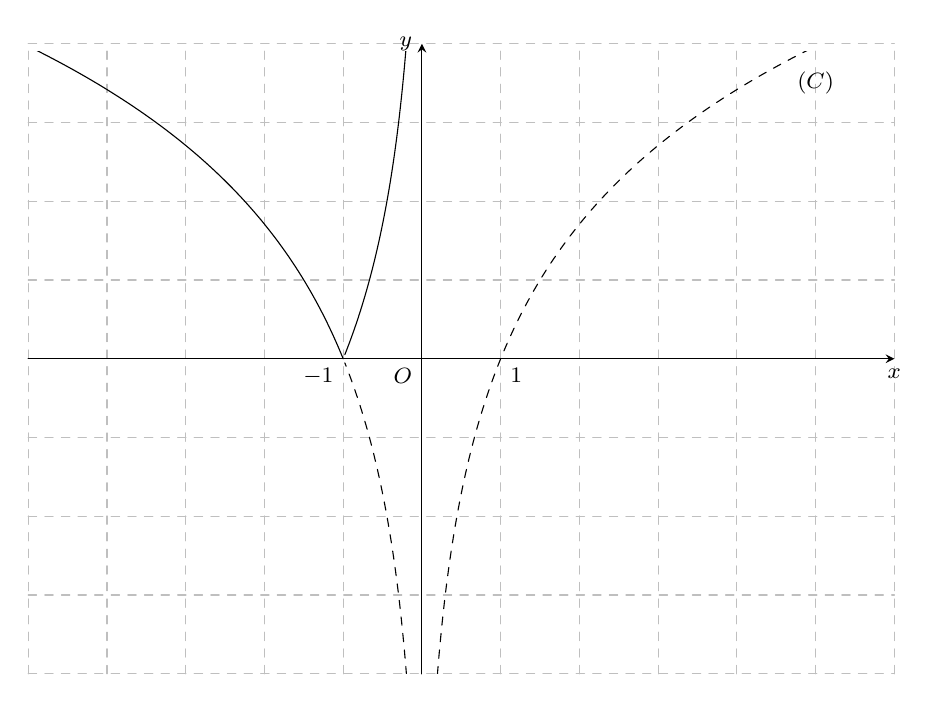
\begin{tikzpicture}[scale=1,>=stealth, font=\footnotesize, line join=round, line cap=round,declare function={hsf(\x)=ln(\x)/ln(1.5);}]
                \def\xmax{6} \def\ymin{-4} \def\ymax{4}
                \draw[color=gray!50,dashed] (-5,\ymin) grid (\xmax,\ymax);
                \draw[->] (-5,0)--(\xmax,0) node [below]{$x$};
                \draw[->] (0,\ymin)--(0,\ymax) node [left]{$y$};
                \node at (0,0) [below left]{$O$}
                (1,0)node[below right]{$1$}
                (-1,0)node[below left]{$-1$};
                \clip (-5,\ymin) rectangle (\xmax-0.1,\ymax-0.1);
                \path(5,3.5)node{$(C)$};
                \draw[smooth,samples=300,domain=0.03:\xmax,dashed] plot(\x,{hsf(\x)});
                \draw[smooth,samples=300,domain=-0.03:-0.98,dashed] plot(\x,{hsf(abs(\x))});
                \draw[smooth,samples=300,domain=-0.03:-0.98] plot(\x,{abs(hsf(abs(\x)))});
                \draw[smooth,samples=300,domain=-1:-\xmax] plot(\x,{hsf(abs(\x))});
            \end{tikzpicture}
        \end{center}
        Ta có hàm số $y=\log _{2018}x$ có tập xác định $D=(0 ;+\infty)$ là hàm số đồng biến trên $(0 ;+\infty)$.\\
        Vì $\left(C'\right)$ đối xứng với $(C)$ qua trục tung nên hàm số $y=f(x)$ là hàm số nghịch biến trên $(-\infty ; 0)$.\\
        Ta có $|f(x)|=\heva{&f(x) &&\text{khi}~f(x) \geq 0 \\& -f(x) &&\text{khi}~f(x)<0}$ nên suy ra đồ thị hàm số $y=|f(x)|$.\\
        Dựa vào đồ thị $y=|f(x)|$ ta suy ra hàm số $y=|f(x)|$ đồng biến trên $(-1 ; 0)$.
    }
\end{ex}
\begin{ex}%[2D2K4-3]
    Có bao nhiêu giá trị thực $ m$ để hàm số $ g(x)=\dfrac{2019^x}{\ln 2019}+\dfrac{6^x}{\ln 6}+\dfrac{m}{2}{x^2}-2x$ đồng biến trên $\mathbb{R}$.
    \choice
    {\True Duy nhất}
    {Không tồn tại}
    {$2019$}
    {Vô số}
    \loigiai{
        Ta có $g'(x)=2019^x+6^x+mx-2$.\\
        Hàm số $ g(x)$ đồng biến trên $\mathbb{R}$ khi và chỉ khi $g'(x)\ge 0,\forall x\in\mathbb{R}$.\\
        Ta có $g'(0)=0$, $\forall m$.
        \begin{itemize}
            \item Nếu $ m\ge 0\Rightarrow\heva{&{g}'(x)=\left(2019^x+6^x-2\right)+mx\ge 0, \forall x\ge 0\\& {g}'(x)=\left(2019^x+6^x-2\right)+mx<0, \forall x<0}$.\\
            Suy ra hàm số đồng biến trên khoảng $\left(0;+\infty\right)$.\\
            $\Rightarrow m\ge 0$ (loại).
            \item Nếu $ m<0$.\\
            Xét $g''(x)=2019^x\ln 2019+6^x\ln 6+m$ là hàm số đồng biến trên $\mathbb{R}$\\
            $\underset{x\to-\infty}{\lim}\left(2019^x\ln 2019+6^x\ln 6\right)=0\Rightarrow $ phương trình $g''(x)=0$ có nghiệm duy nhất $ x=x_0$\\
            khi $ m<0$ và $g'(x)$ đạt GTNN tại điểm cực tiểu duy nhất tại $ x=x_0$.\\
            Do đó, để $g'(x)\ge 0,\forall x\in\mathbb{R}$ thì $g'\left(x_0\right)\ge 0$.\\
            Mà $g'(0)=0\Rightarrow{x_0}=0\Rightarrow m=-2019^0\ln 2019-6^0\ln 6$ hay $ m=-\ln 2019-\ln 6$.\\
            Do đó có duy nhất một giá trị thực của $ m$ thỏa mãn.
        \end{itemize}
    }
\end{ex}
\begin{ex}%[2D2K4-3]
    Tập các giá trị của tham số $ m$ để hàm số $ y=\ln \left(3x-1\right)-\dfrac{m}{x}+2$ đồng biến trên khoảng $\left(\dfrac{1}{2};+\infty\right)$ là
    \choice
    {$\left[\dfrac{2}{9};+\infty\right)$}
    {\True $\left[-\dfrac{4}{3};+\infty\right)$}
    {$\left[-\dfrac{7}{3};+\infty\right)$}
    {$\left[-\dfrac{1}{3};+\infty\right)$}
    \loigiai{
        $ y=\ln \left(3x-1\right)-\dfrac{m}{x}+2\Rightarrow y'=\dfrac{3}{3x-1}+\dfrac{m}{x^2}$.\\
        Để hàm số đồng biến trên khoảng $\left(\dfrac{1}{2};+\infty\right)\Leftrightarrow y'\ge 0,\forall x\in\left(\dfrac{1}{2};+\infty\right)$
        \begin{align*}
            &\dfrac{3}{3x-1}+\dfrac{m}{x^2}\ge 0,\forall x\in\left(\dfrac{1}{2};+\infty\right)\\
            \Leftrightarrow& m\ge\dfrac{3x^2}{1-3x}=g(x),\forall x\in\left(\dfrac{1}{2};+\infty\right).
        \end{align*}
        Xét $g(x)=\dfrac{3x^2}{1-3x},\forall x\in\left(\dfrac{1}{2};+\infty\right)\Rightarrow g'(x)=\dfrac{6x-9x^2}{\left(1-3x\right)^2}$.\\
        Khi đó $ g'(x)=0\Leftrightarrow \hoac{& x=0 \\ & x=\dfrac{2}{3}.}$\\
        Bảng biến thiên
        \begin{center}
            
\begin{tikzpicture}[>=stealth]
                \tkzTabInit[nocadre=false,lgt=1.2,espcl=2.5,deltacl=0.5]{$x$/1,$g'(x)$/.7,$g(x)$/2}
                {$\dfrac{1}{2}$ , $\dfrac{2}{3}$ , $+\infty$}
                \tkzTabLine{ , + , $0$ , - , }
                \tkzTabVar{-/ , +/$-\dfrac{4}{3}$ , -/}
            \end{tikzpicture}
        \end{center}
        Vậy $ m\ge-\dfrac{4}{3}\Leftrightarrow m\in\left[-\dfrac{4}{3};+\infty\right)$.
    }
\end{ex}
\begin{ex}%[2D2K4-3]
    [Chuyên Lê Quý Đôn Quảng Trị 2019]%Câu 53
    \immini{
        Cho các hàm số $y=\log_a x$ và $y=\log_bx$ có đồ thị như hình vẽ bên. Đường thẳng $x=6$ cắt trục hoành, đồ thị hàm số $y=\log_a x$ và $y=\log_bx$ lần lượt tại $A$, $B$ và $C$. Nếu $AC=AB\log_23$ thì
        \choice
        {$b^3=a^2$}
        {\True $\log_2b=\log_3a$}
        {$b^2=a^3$}
        {$\log_3b=\log_2a$}
    }{
        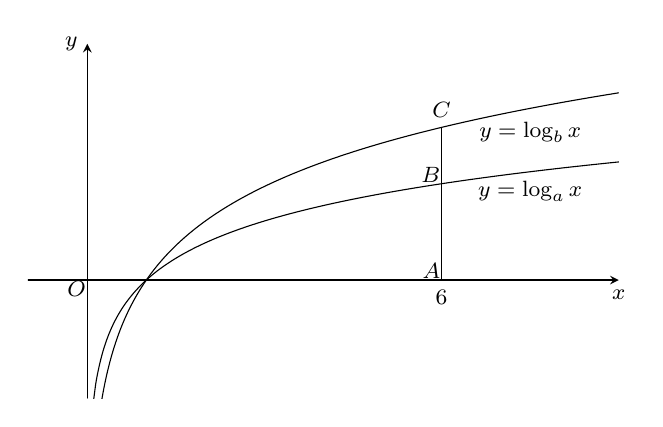
\begin{tikzpicture}[scale=0.75, font=\footnotesize, line join=round, line cap=round,>=stealth]
            \draw[->] (-1,0) --(9,0) node[below]{$x$};
            \draw[->] (0,-2) --(0,4) node[left]{$y$};
            %\draw (0,0) rectangle (1/4,1/4);
            \draw (0,0) node[below left=-3pt]{$O$};
            \begin{scope}
                \clip (-1,-2) rectangle (9,4);
                \draw [smooth,domain=0.1:9, samples=200] plot (\x, {(ln(\x))/(ln(2))});
                \draw [smooth,domain=0.1:9, samples=200] plot (\x, {(ln(\x))/(ln(3))});
                \draw (6,0)--(6,2.585);
            \end{scope}
            \draw (6,0)node[below]{$6$} (6,0)node[above left=-3pt]{$A$} (6,1.631)node[above left=-3pt]{$B$} (6,2.585)node[above]{$C$};
            \draw (7.5, 1.5)node{$y=\log_ax$} (7.5, 2.5)node{$y=\log_bx$};
        \end{tikzpicture}
    }
    \loigiai{
        Ta có $A(6;0)$, $B(6;\log_a6)$ và $C(6;\log_b6)$, suy ra $AB=\log_a6$, $AC=\log_b6$.\\
        Do đó $AC=AB\log_23\Leftrightarrow \log_b6=\log_a6\cdot \log_23\Leftrightarrow \log_b6=\log_ab\cdot \log_b6\cdot \log_23.\quad (1)$\\
        Vì $\log_b6\neq 0$ nên $(1)\Leftrightarrow \log_ab\cdot \log_23=1\Leftrightarrow \dfrac{\log_3b\cdot \log_23}{\log_3a}=1\Leftrightarrow \log_2b=\log_3a$.
    }
\end{ex}
\begin{ex}%[2D2B4-7]
    \immini{
        Trong hình bên, đường cong là đồ thị của hàm số $y=\ln x$, điểm $B$ là trung điểm của đoạn thẳng $AC$. Khẳng định nào sau đây là đúng?
        \choice
        {$a+c=2b$}
        {$ac=b$}
        {$ac=2b^2$}
        {\True $ac=b^2$}
    }{
        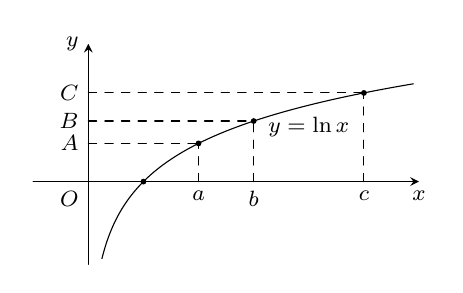
\begin{tikzpicture}[scale=0.7, font=\footnotesize, line join=round, line cap=round, >=stealth]
            \def\xt{-1} \def\xp{6} \def\yt{2.5} \def\yd{-1.5} % x_trái, x_phải, y_trên, y_dưới (giới hạn)
            \draw[->] (\xt,0)--(\xp,0) node [below]{$x$};
            \draw[->] (0,\yd)--(0,\yt) node [left]{$y$};
            \node at (0,0) [below left]{$O$}; \node at (4,1.35) [below]{$y=\ln x$};
            \clip (\xt-0.1,\yd+0.1) rectangle (\xp-0.1,\yt-0.1);
            \draw[smooth,samples=300,domain=0.1:\xp] plot(\x,{ln(\x)});
            \draw[dashed] (2,0) node [below]{$a$}--(2,0.693) (0,0.693) node [left]{$A$}--(2,0.693) (3,0) node [below]{$b$}--(3,1.099) (0,1.099) node [left]{$B$}--(3,1.099) (5,0) node [below]{$c$}--(5,1.609) (0,1.609) node [left]{$C$}--(5,1.609);
            \fill (1,0) circle (1.5pt) (2,0.693) circle (1.5pt) (3,1.099) circle (1.5pt) (5,1.609) circle (1.5pt);
        \end{tikzpicture}
    }
    \loigiai{
        Ta có $A\left(0;\ln a\right)$, $B\left(0;\ln b\right)$, $C\left(0;\ln c\right)$.\\
        Do $B$ là trung điểm của đoạn thẳng $AC$ nên
        $$\ln a+\ln c=2\ln b \Leftrightarrow \ln (ac)=\ln (b^2) \Leftrightarrow ac=b^2.$$
    }
\end{ex}
\begin{ex}%[2D2B4-3]
    Đồ thị hàm số $y=f(x)$ đối xứng với đồ thị hàm số $y=a^x$, $\left(a>0,a\ne 1\right)$ qua điểm $I(1;1)$. Giá trị của biểu thức $f\left(2+\log_a\dfrac{1}{2018}\right)$ bằng
    \choice
    {$2016$}
    {\True $-2016$}
    {$2020$}
    {$-2020$}
    \loigiai{
        Gọi $(C)$ là đồ thị hàm số $y=a^x$; $\left(C_1\right)$ là đồ thị hàm số $y=f(x)$.\\
        $M\left(2+\log_a\dfrac{1}{2018};{y_M}\right)\in\left(C_1\right)$ $\Leftrightarrow{y_M}=f\left(2+\log_a\dfrac{1}{2018}\right)$.\\
        Gọi $N$ đối xứng với $M$ qua $I\left(1;1\right)$ $\Rightarrow N\left(-\log_a\dfrac{1}{2018};2-y_M\right)$.\\
        Do đồ thị $\left(C_1\right)$ đối xứng $(C)$ qua $I\left(1;1\right)$ nên $N\left(-\log_a\dfrac{1}{2018};2-y_M\right)\in(C)$.\\
        $N\in(C)$ $\Leftrightarrow 2-y_M=a^{-\log_a\dfrac{1}{2018}}$ $\Leftrightarrow 2-y_M=a^{\log_a2018}$ $\Leftrightarrow 2-y_M=2018$ $\Leftrightarrow{y_M}=-2016$.\\
        Vậy $f\left(2+\log_a\dfrac{1}{2018}\right)=-2016$.
    }
\end{ex}
\begin{ex}%[2D2K4-3]
    [Hội 8 trường chuyên ĐBSH - 2019]%Câu 56
    \immini
    {
        Cho số thực dương $a$ khác $1$. Biết rằng bất kỳ đường thẳng nào song song với trục $Ox$ mà cắt các đường $y=4^x$, $y=a^x$, trục tung lần lượt tại $M$, $N$ và $A$ thì $AN=2AM$ (hình vẽ bên). Giá trị của $a$ bằng
        \choice
        {$\dfrac{1}{3}$}
        {$\dfrac{\sqrt{2}}{2}$}
        {$\dfrac{1}{4}$}
        {\True $\dfrac{1}{2}$}
    }
    {
        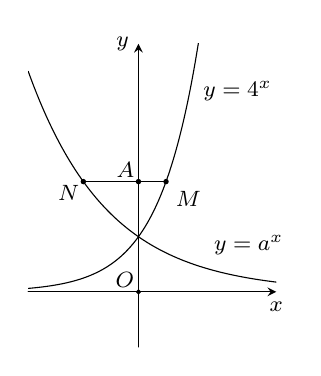
\begin{tikzpicture}[scale=0.7, font=\footnotesize, line join=round, line cap=round, >=stealth]
            \draw[->] (-2,0)--(2.5,0) node[below]{$x$} ;
            \draw[->] (0,-1)--(0,4.5) node[left]{$y$};
            \draw[fill=black] (0,0) circle(1pt) node[above left=-2pt] {$O$} ;
            \draw[fill=black] (1,4) node[below right]{$y=4^x$} (2,0.5) node[above]{$y=a^x$} (0.5,2) circle (1.1pt) node[below right]{$M$} (0,2) circle (1.1pt) node[above left=-2pt]{$A$} (-1,2) circle (1.1pt) node[below left=-2pt]{$N$};
            \draw (0.5,2)--(-1,2) ;
            \clip (-2,-1) rectangle (2.5,4.5) ;
            \draw[smooth, samples=100, domain=-2:2.5] plot(\x,{exp(ln(4)*(\x))}) ;
            \draw[smooth, samples=100, domain=-2:2.5] plot(\x,{exp(ln(0.5)*(\x))}) ;
        \end{tikzpicture}
    }
    \loigiai{
        Dựa vào ĐTHS ta thấy hàm số $y=a^x$ nghịch biến nên $0<a<\dfrac{1}{2}$.\\
        Mọi đường thẳng $y=m$, $m>0$ đều cắt các đường $y=4^x$, $y=a^x$, trục tung lần lượt tại $M\left(\log_4m;m\right)$, $N\left(\log_am;m\right)$ và $A=(0;m)$, theo bài ra
        \begin{align*}
            AN=2AM\Leftrightarrow&\left|\log_am\right|=2\left|\log_4m\right|\Leftrightarrow\left|\log_am\right|=\left|\log_2m\right|\\
            \Leftrightarrow&\hoac{&{\log_a}m=\log_2m\\& {\log_a}m=-\log_2m}\\
            \Leftrightarrow&\hoac{&{\log_m}a=\log_m2\\& {\log_m}a=\log_m\dfrac{1}{2}}\\
            \Leftrightarrow&\hoac{& a=2\\&  a=\dfrac{1}{2}.}
        \end{align*}
        Vậy $a=\dfrac{1}{2}$.
    }
\end{ex}
\begin{ex}%[2D2B4-3]
    [THPT Ngô Quyền - Ba Vì - Hải Phòng 2019]%Câu 57
    Đồ thị hàm số $y=f(x)$ đối xứng với đồ thị hàm số $ y=\log_ax$, $\left(0<a\ne 1\right)$ qua điểm $ I\left(2;1\right)$. Giá trị của biểu thức $ f\left(4-a^{2019}\right)$ bằng
    \choice
    {$2023$}
    {$-2023$}
    {$2017$}
    {\True $-2017$}
    \loigiai{
        Lấy điểm $A\left(4-a^{2019};f\left(4-a^{2019}\right)\right)$ thuộc đồ thị của hàm số $ y=f(x)$ và điểm $B\left(x;\log_ax\right)$ thuộc đồ thị của hàm số $ y=\log_ax$.\\
        Hai điểm $ A$ và $ B$ đối xứng nhau qua điểm $ I$ khi và chỉ khi\\
        $\heva{& 4-a^{2019}+x=4\\&  f\left(4-a^{2019}\right)+\log_ax=2}\Leftrightarrow\heva{& x=a^{2019}\\&  f\left(4-a^{2019}\right)+\log_a{a^{2019}}=2}\Rightarrow f\left(4-a^{2019}\right)=-2017$.
    }
\end{ex}
\begin{ex}%[2D2G4-3]%
    \immini{
        Hàm số $y=\log_a x, y=\log_b x$ có đồ thị như hình vẽ dưới đây. Đường thẳng $x=5$ cắt trục hoành, hai đồ thị $y=\log_a x$, $y=\log_b x$ lần lượt tại các điểm $A$, $B$, $C$. Biết rằng $CB=2AB$. Mệnh đề nào dưới đây là đúng?
        \choice
        {$a=b^2$}
        {$a^3=b$}
        {\True $a=b^3$}
        {$a=5b$}
    }
    {
        \begin{tikzpicture}[>=stealth,scale=0.8, line join=round, line cap=round]
            \draw[->] (-1,0)--(6,0) node [below]{$x$};
            \draw[->] (0,-1)--(0,8) node [left]{$y$};
            \node at (0,0) [below left]{$O$};
            \clip (-3,-1) rectangle (7,8);
            \fill[black] (1,0) circle (2pt) node [below right] {$1$}
            (5,{ln(5)/ln((2)^(1/3))}) circle (2pt) node [right]{$C$}
            (5,{ln(5)/ln(2)}) circle (2pt) node [below right]{$B$}
            (5,0) circle (2pt)node [below right]{$A$} ;
            \draw[smooth,samples=150,domain=0.1:6] plot(\x,{ln(\x)/ln(2)});
            \draw[smooth,samples=150,domain=0.1:6] plot(\x,{ln(\x)/ln((2)^(1/3))});
            \node at (2.5,2.5)[right]{$y=\log_ax$};
            \node at (2.2,6){$y=\log_bx$};
            \draw (5,-1)--(5,8) node [below left]{$x=5$} ;

        \end{tikzpicture}

    }
    \loigiai{
        $\log_b 5=3\log_a 5 \Leftrightarrow \log_5 a=3\log_5 b$. Vậy $a=b^3$.
    }
\end{ex}
\begin{ex}%[2D2B4-3]
    [THPT Đông Sơn 1 - Thanh Hóa - 2019]%Câu 59
    Cho hàm số $ f(x)=\dfrac{4^x}{4^x+2}$. Tính giá trị biểu thức $ A=f\left(\dfrac{1}{100}\right)+f\left(\dfrac{2}{100}\right)+\ldots+f\left(\dfrac{100}{100}\right)?$
    \choice
    {$ 50$}
    {$ 49$}
    {$\dfrac{149}{3}$}
    {\True $\dfrac{301}{6}$}
    \loigiai{
        Xét hai số dương $ a$ và $ b$ sao cho $a+b=1$, ta có
        \allowdisplaybreaks
        \begin{align*}
            f(a)+f(b)=&\dfrac{4^a}{4^a+2}+\dfrac{4^b}{4^b+2}\\
            =&\dfrac{4^a\left(4^b+2\right)+4^b\left(4^a+2\right)}{\left(4^a+2\right)\left(4^b+2\right)}\\
            =&\dfrac{2\left(4^{a+b}+4^a+4^b\right)}{4^{a+b}+2\left(4^a+4^b\right)+4}\\
            =&\dfrac{2\left(4+4^a+4^b\right)}{2\left(4+4^a+4^b\right)}\\
            =&1
        \end{align*}
        Do đó
        \begin{align*}
            A=&\left[f\left(\dfrac{1}{100}\right)+f\left(\dfrac{99}{100}\right)\right]+\ldots+\left[f\left(\dfrac{49}{100}\right)+f\left(\dfrac{51}{100}\right)\right]+f\left(\dfrac{50}{100}\right)+f\left(\dfrac{100}{100}\right)\\
            =&49+f\left(\dfrac{1}{2}\right)+f(1)=\dfrac{301}{6}.
        \end{align*}
        Vậy $ A=\dfrac{301}{6}$.
    }
\end{ex}
\begin{ex}%[2D2K4-3]
    Tìm tập hợp tất cả các giá trị của tham số thực $m$ đề hàm số $ y=\ln \left(x^2+1\right)-mx+1$ đồng biến trên $\mathbb{R}$.
    \choice
    {$\left[-1;1\right]$}
    {$\left(-1;1\right)$}
    {\True $\left(-\infty ;-1\right]$}
    {$\left(-\infty ;-1\right)$}
    \loigiai{
        Tập xác định $\mathscr{D}=\mathbb{R}$. Ta có $y'=\dfrac{2x}{x^2+1}-m$.\\
        Hàm số $ y=\ln \left(x^2+1\right)-mx+1$ đồng biến trên R khi $ y'\ge0\forall x\in \mathbb{R}$\\
        $$\Leftrightarrow\dfrac{2x}{x^2+1}-m\ge0\forall x\in \mathbb{R}\Leftrightarrow\dfrac{2x}{x^2+1}\ge m\forall x\in \mathbb{R}.$$\\
        Xét hàm $ f(x)=\dfrac{2x}{x^2+1}$. Ta có $ f'(x)=\dfrac{-2x^2+2}{\left(x^2+1\right)^2}$.\\
        $f'(x)=0\Leftrightarrow\dfrac{-2x^2+2}{\left(x^2+1\right)^2}=0\Leftrightarrow x=\pm1$.\\
        Bảng biến thiên
        \begin{center}
            
\begin{tikzpicture}[>=stealth]
                \tkzTabInit[nocadre=false,lgt=1.2,espcl=2.5,deltacl=0.5]{$x$/.7 ,$f'(x)$/.7,$f(x)$/3}
                {$-\infty$ , $-1$ , $1$ , $+\infty$}
                \tkzTabLine{ , - , $0$ , + , $0$ , - , }
                \tkzTabVar{+/$0$ , -/$-1$ , +/$1$ , -/$0$}
            \end{tikzpicture}
        \end{center}
        Dựa vào bảng biến thiến suy ra $-1\le f(x)\le1, \forall x\in \mathbb{R}$.\\
        Từ đó suy ra $m\le-1$.
    }
\end{ex}
\begin{ex}%[2D2K4-1]
    Có bao nhiêu giá trị nguyên của $ m$ thuộc khoảng $\left(-2019;2019\right)$ để hàm số sau có tập xác định là $ \mathscr{D}=\mathbb{R}$?\\
    \centerline{$y=x+m+\sqrt{x^2+2\left(m+1\right)x+m^2+2m+4}+\log_2\left(x-m+\sqrt{2x^2+1}\right)$}
    \choice
    {$2020$}
    {$2021$}
    {$2018$}
    {\True $2019$}
    \loigiai{
        Hàm số xác định với mọi $x\in\mathbb{R}$ thì $\heva{& x^2+2(m+1)x+m^2+2m+4\ge 0\\&  x-m+\sqrt{2x^2+1}>0}$ luôn đúng với mọi $x\in\mathbb{R}$.\\
        Ta có $x^2+2(m+1)x+m^2+2m+4=\left[x+\left(m+1\right)\right]^2+3>0$, $\forall x\in\mathbb{R}$.\\
        Ta có $ x-m+\sqrt{2x^2+1}>0$, $\forall x\in\mathbb{R}$.\\
        $\Leftrightarrow x+\sqrt{2x^2+1}>m$, $\forall x\in\mathbb{R}$.\\
        Xét hàm số $ f(x)=x+\sqrt{2x^2+1}$ với $x\in\mathbb{R}$.\\
        $f'(x)=1+\dfrac{2x}{\sqrt{2x^2+1}}$.\\
        $f'(x)=0\Leftrightarrow x=\dfrac{-1}{\sqrt{2}}$.
        \begin{center}
            
\begin{tikzpicture}[>=stealth]
                \tkzTabInit[nocadre=false,lgt=1.2,espcl=2.5,deltacl=0.5]{$x$/1,$y'$/.7,$y$/3}
                {$-\infty$ , $\dfrac{-1}{\sqrt{2}}$ , $+\infty$}
                \tkzTabLine{ , - , $0$ , + , }
                \tkzTabVar{+/$+\infty$ , -/$\dfrac{\sqrt{2}}{2}$ , +/$+\infty$}
            \end{tikzpicture}
        \end{center}
        Từ bảng biến thiên ta thấy để $ x+\sqrt{2x^2+1}>m,\forall x\in\mathbb{R}\Leftrightarrow\dfrac{\sqrt{2}}{2}>m$.\\
        Kết hợp điều kiện
        $\heva{& m\in\mathbb{Z}\\&  m\in\left(-2019;2019\right)}\Rightarrow m \in \{-2018,-2017,-2016,\ldots,-1,0\}$.\\
        Kết luận có $2019$ giá trị của $m$ thỏa mãn bài toán.
    }
\end{ex}
\begin{ex}%[2D2K4-3]
    [THPT Yên Dũng 2 - Bắc Giang 2019]
    Tập tất cả các giá trị của tham số $m$ để hàm số $ y=\dfrac{m\ln x-2}{\ln x-m-1}$ nghịch biến trên $\left(\mathrm{e}^2;+\infty\right)$ là
    \choice
    {$\hoac{& m\le-2\\&  m=1}$}
    {$\hoac{& m<-2\\&  m>1}$}
    {$\hoac{& m<-2\\&  m=1}$}
    {\True $ m<-2$}
    \loigiai{
        Điều kiện xác định $\heva{& x>0\\&  x\ne{\mathrm{e}^{m+1}}}$.\\
        Ta có $y'=\dfrac{\frac{m}{x}\left(\ln x-m-1\right)-\frac{1}{x}\left(m\ln x-2\right)}{\left(\ln x-m-1\right)^2}=\dfrac{-m^2-m+2}{x{\left(\ln x-m-1\right)^2}}$.\\
        Hàm số nghịch biến trên $\left(\mathrm{e}^2;+\infty\right)$ khi và chỉ khi $$\heva{&-m^2-m+2<0\\& \mathrm{e}^{m+1}\le{\mathrm{e}^2}}\Leftrightarrow \heva{&\hoac{& m<-2\\&  m>1}\\& m+1\le 2}\Leftrightarrow m<-2.$$
    }
\end{ex}
\begin{ex}%[2D2K4-3]
    [Chuyên Bắc Giang 2019]
    Có bao nhiêu giá trị nguyên của $ m$ thuộc khoảng $\left(-2019;2019\right)$ để hàm số $ y=2019^{x^3-x^2-mx+1}$ nghịch biến trên $[-1;2]$
    \choice
    {$2020$}
    {$2019$}
    {$2010$}
    {\True $2011$}
    \loigiai{
        $y'=\left(3x^2-2x-m\right){2019^{x^3-x^2-mx+1}}\cdot\ln 2019$.\\
        Hàm số nghịch biến trên $[-1;2]$ $\Leftrightarrow y'\le 0,\forall x\in\left[-1;2\right]$.\\ $\Leftrightarrow 3x^2-2x-m\le 0\forall x\in\left[-1;2\right]$.\\
        $\Leftrightarrow 3x^2-2x\le m\forall x\in\left[-1;2\right]$.\\
        Đặt $f(x)=3x^2-2x$; $f'(x)=6x-2$.\\
        Bảng biến thiên
        \begin{center}
            
\begin{tikzpicture}[>=stealth]
                \tkzTabInit[nocadre=false,lgt=1.2,espcl=2.5,deltacl=0.5]{$x$/1,$f'(x)$/.7,$f(x)$/2}
                {$-1$, $\dfrac{1}{3}$, $2$}
                \tkzTabLine{ , - , $0$ , + , }
                \tkzTabVar{+/$5$ , -/$-\dfrac{1}{3}$ , +/$8$}
            \end{tikzpicture}
        \end{center}
        Từ bảng biến thiên suy ra $ f(x)\le 8\forall x\in\left[-1;2\right]$.\\
        Do đó $\Leftrightarrow m\ge 8$.\\
        Vì $m$ nguyên thuộc khoảng $\left(-2019;2019\right)$ nên có $2011$ giá trị $m$ thỏa mãn.
    }
\end{ex}
\begin{ex}%[2D2K4-3]
    [Hậu Lộc 2 - Thanh Hóa-2019]%Câu 64
    \immini{
        Cho $a$, $b$ là các số thực dương khác $1$, đồ thị hàm số $y=\log_ax$ và $y=\log_bx$ lần lượt là $\left(C_1\right)$, $\left(C_2\right)$ như hình vẽ.\\
        Khẳng định nào sau đây là đúng
        \choice
        {$\mathrm{e}$}
        {$ b\cdot\mathrm{e}^a>a\cdot\mathrm{e}^b$}
        {$ b\cdot\mathrm{e}^a=a\cdot\mathrm{e}^b$}
        {\True $ a\cdot\mathrm{e}^a<b\cdot\mathrm{e}^b$}
    }
    {
        \begin{tikzpicture}[scale=.7,>=stealth, font=\footnotesize, line join=round, line cap=round]
            \def\xmax{6} \def\ymin{-4} \def\ymax{4}
            \draw[->] (-0.9,0)--(\xmax,0) node [below]{$x$};
            \draw[->] (0,\ymin)--(0,\ymax) node [left]{$y$};
            \node at (0,0) [below left]{$O$};
            \clip (-0.9,\ymin) rectangle (\xmax-0.1,\ymax-0.1);
            \draw[smooth,samples=300,domain=0.03:\xmax] plot(\x,{ln(\x)/ln(.3)})node[above left]{$(C_1)$};
            \draw[smooth,samples=300,domain=0.03:5] plot(\x,{ln(\x)/ln(.6)})node[below left]{$(C_2)$};
        \end{tikzpicture}
    }
    \loigiai{
        Ta có $\log_ax=1\Leftrightarrow x=a$ và $\log_bx=1\Leftrightarrow x=b$.\\
        Nên kẻ đường thẳng $ y=1$ cắt đồ thị $\left(C_1\right)$, $\left(C_2\right)$ lần lượt tại các điểm có tọa độ $\left(a;1\right)$ và $\left(b;1\right)$.
        \begin{center}
            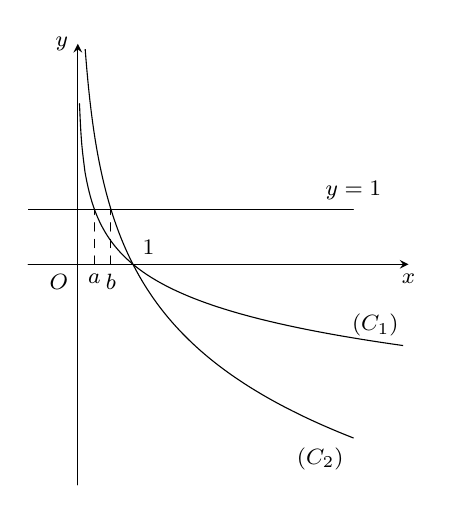
\begin{tikzpicture}[scale=.7,>=stealth, font=\footnotesize, line join=round, line cap=round]
                \def\xmax{6} \def\ymin{-4} \def\ymax{4}
                \draw[->] (-0.9,0)--(\xmax,0) node [below]{$x$};
                \draw[->] (0,\ymin)--(0,\ymax) node [left]{$y$};
                \node at (0,0) [below left]{$O$};
                \clip (-0.9,\ymin) rectangle (\xmax-0.1,\ymax-0.1);
                \draw (-1,1)--(5,1)node[above]{$y=1$}
                (1,0)node[above right]{$1$};
                \draw[dashed] (0.3,0)node[below]{$a$}--++(90:1)
                (0.6,0)node[below]{$b$}--++(90:1)
                ;
                \draw[smooth,samples=300,domain=0.03:\xmax] plot(\x,{ln(\x)/ln(.3)})node[above left]{$(C_1)$};
                \draw[smooth,samples=300,domain=0.03:5] plot(\x,{ln(\x)/ln(.6)})node[below left]{$(C_2)$};
            \end{tikzpicture}
        \end{center}
        Nhìn vào đồ thị ta suy ra $ a<b$.\\
        Do $a$, $ b$, $\mathrm{e}^a$, $\mathrm{e}^b$ là các số dương và $\mathrm{e}>1$ nên từ $a<b$ ta suy ra
        $$\heva{&{\mathrm{e}^a}<\mathrm{e}^b\\&  a\cdot\mathrm{e}^b<b\cdot\mathrm{e}^b}\Rightarrow\heva{& a\cdot\mathrm{e}^a<a\cdot\mathrm{e}^b\\&  a\cdot\mathrm{e}^b<b\cdot\mathrm{e}^b}\Rightarrow a\cdot\mathrm{e}^a<b\cdot\mathrm{e}^b.$$
    }
\end{ex}
\begin{ex}%[2D2B4-3]
    [Liên trường huyện Quảng Xương - Thanh Hóa - 2021]%Câu 65
    \immini
    {
        Cho ba số thực dương $a$, $b$, $c$ khác $1$.\\
        Đồ thị các hàm số $y=a^x$, $ y=b^x$ và $ y=c^x$ được cho như hình vẽ bên. Mệnh đề nào dưới đây đúng?
        \choice
        {$ 1<a<b<c$}
        {$ 1<a<c<b$}
        {$ 0<a<1<b<c$}
        {\True $ 0<a<1<c<b$}
    }
    {
        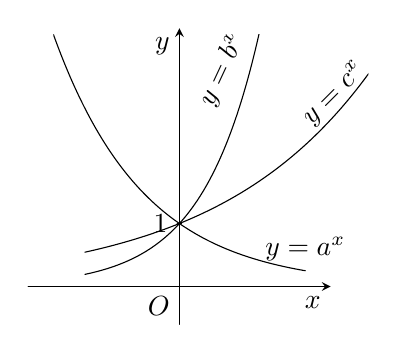
\begin{tikzpicture}[scale=0.8,line join=round, line cap=round,>=stealth]
            \tikzset{label style/.style={font=\footnotesize}}
            \draw[->] (-2.4,0)--(2.4,0) node[below left] {$x$};
            \draw[->] (0,-0.6)--(0,4.1) node[below left] {$y$};
            \draw (0,0) node [below left] {$O$};
            \foreach \y in {1}
            \draw (1pt,\y)--(-1pt,\y) node [left] {$\y$};
            \begin{scope}
                \clip (-2,-0.5) rectangle (3,4);
                \draw[samples=200,domain=-3:2,smooth,variable=\x] plot (\x,{(1/2)^(\x)})node[above]{$ y=a^x $};
                \draw[samples=200,domain=-1.5:2,smooth,variable=\x] plot (\x,{3^(\x)}) (1.0,3.3) node[rotate=65,above]{$ y=b^x $};
                \draw[samples=200,domain=-1.5:4,smooth,variable=\x] plot (\x,{1.5^(\x)}) (3,3.6) node[rotate=45,left]{$y= c^x $};
            \end{scope}
        \end{tikzpicture}
    }
    \loigiai{
        \begin{center}
            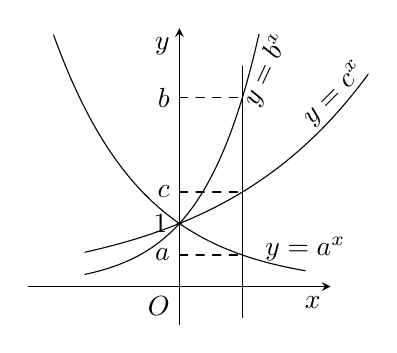
\begin{tikzpicture}[scale=0.8,line join=round, line cap=round,>=stealth]
                \tikzset{label style/.style={font=\footnotesize}}
                \draw[->] (-2.4,0)--(2.4,0) node[below left] {$x$};
                \draw[->] (0,-0.6)--(0,4.1) node[below left] {$y$};
                \draw (0,0) node [below left] {$O$};
                \foreach \y in {1}
                \draw (1pt,\y)--(-1pt,\y) node [left] {$\y$};
                \begin{scope}
                    \clip (-2,-0.5) rectangle (3,4);
                    \draw[samples=200,domain=-3:2,smooth,variable=\x] plot (\x,{(1/2)^(\x)})node[above]{$ y=a^x $};
                    \draw[samples=200,domain=-1.5:2,smooth,variable=\x] plot (\x,{3^(\x)}) (1.7,3.3) node[rotate=65,above]{$ y=b^x $};
                    \draw[samples=200,domain=-1.5:4,smooth,variable=\x] plot (\x,{1.5^(\x)}) (3,3.6) node[rotate=45,left]{$y= c^x $};
                    \draw (1,-.5)--++(90:4);
                    \draw[dashed] (0,.5)node[left]{$a$}--++(0:1)
                    (0,1.5)node[left]{$c$}--++(0:1)
                    (0,3)node[left]{$b$}--++(0:1)
                    ;
                \end{scope}
            \end{tikzpicture}
        \end{center}
        Kẻ đường thẳng $ x=1$ cắt đồ thị các hàm số tại các điểm tương ứng $a$, $b$, $c$.\\
        Từ đồ thị ta có $0<a<1<c<b$.
    }
\end{ex}
\begin{ex}%[2D2B4-3]
    [THPT PTNK Cơ sở 2 - TP.HCM - 2021]%Câu 66
    \immini
    {
        Cho hai số $a,c$ dương và khác $1$. Các hàm số $ y=a^x$, $y=x^b$, $y=\log_cx$ có đồ thị như hình vẽ.\\
        Khẳng định nào sau đây đúng?
        \choice
        {$c<b<a$}
        {$b<a<c$}
        {\True $b<c<a$}
        {$a<c<b$}
    }
    {
        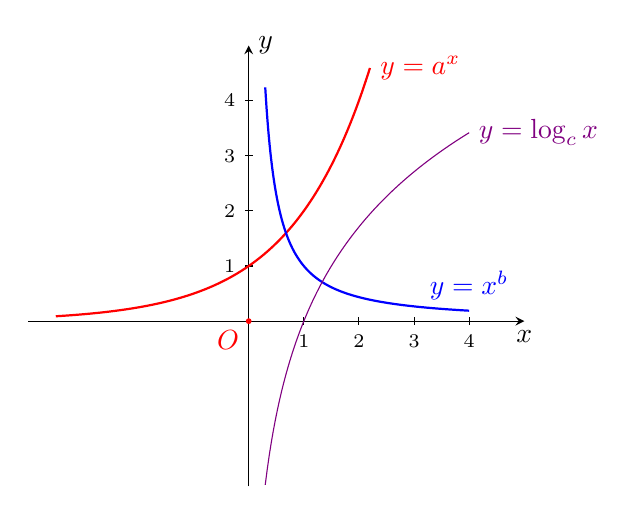
\begin{tikzpicture}[>=stealth,scale=.7,font=\normalfont]
            \draw[->] (-4,0)--(5,0)node[below]{$x$};
            \foreach \x in {1,2,3,4}
            \draw[shift={(\x,0)}] (0,2pt)--(0,-2pt) node[below]{\scriptsize $\x$};
            \draw[->] (0,-3)--(0,5)node[right]{$y$};
            \foreach \y in {1,2,3,4}
            \draw[shift={(0,\y)}] (2pt,0)--(-2pt,0) node[left]{\scriptsize $\y$};
            \fill[red] (0,0)node[below left]{$O$}circle(1.5pt);
            \draw[samples=150,domain=-3.5:2.2,smooth,red,thick] plot (\x, {2^(\x)})node[right]{$y=a^x$};
            \draw[samples=150,domain=0.3:4,smooth,blue,thick] plot (\x, {(\x)^(-1.2)})node[above]{$y=x^b$};
            \draw[violet] plot [domain=0.3:4,samples=100,thick] (\x,{ln(\x)/ln(1.5)})node[right]{$y=\log_c x$};
        \end{tikzpicture}
    }
    \loigiai{
        \begin{center}
            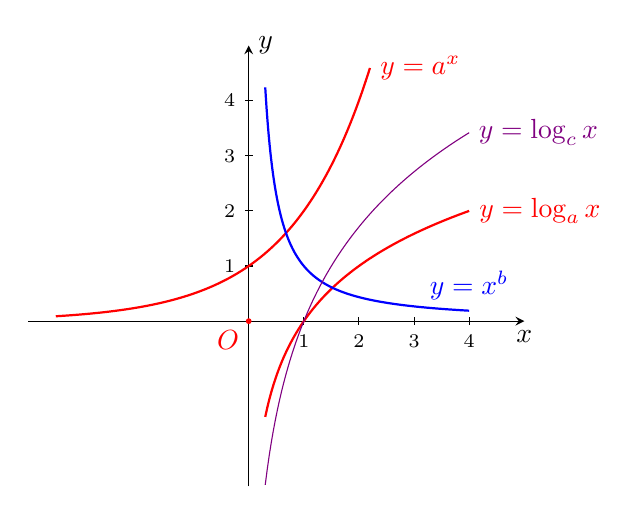
\begin{tikzpicture}[>=stealth,scale=.7,font=\normalfont]
                \draw[->] (-4,0)--(5,0)node[below]{$x$};
                \foreach \x in {1,2,3,4}
                \draw[shift={(\x,0)}] (0,2pt)--(0,-2pt) node[below]{\scriptsize $\x$};
                \draw[->] (0,-3)--(0,5)node[right]{$y$};
                \foreach \y in {1,2,3,4}
                \draw[shift={(0,\y)}] (2pt,0)--(-2pt,0) node[left]{\scriptsize $\y$};
                \fill[red] (0,0)node[below left]{$O$}circle(1.5pt);
                \draw[samples=150,domain=-3.5:2.2,smooth,red,thick] plot (\x, {2^(\x)})node[right]{$y=a^x$};
                \draw[red,thick] plot [domain=0.3:4,samples=100] (\x,{ln(\x)/ln(2)})node[right]{$y=\log_a x$};
                \draw[samples=150,domain=0.3:4,smooth,blue,thick] plot (\x, {(\x)^(-1.2)})node[above]{$y=x^b$};
                \draw[violet] plot [domain=0.3:4,samples=100,thick] (\x,{ln(\x)/ln(1.5)})node[right]{$y=\log_c x$};
            \end{tikzpicture}
        \end{center}
        Từ đồ thị hàm số $ y=x^b$ suy ra $ b<0$.\\
        Ta có đồ thị hàm số $ y=\log_ax$ đối xứng với đồ thị hàm số $ y=a^x$ qua đường thẳng $ y=x$.\\
        Theo đồ thị hàm số $ y=\log_ax,y=\log_cx$ ta có $\log_ax<\log_cx$ và $ a,c>1$ suy ra $ 1<c<a$.\\
        Vậy $ b<c<a$.
    }
\end{ex}
\begin{ex}%[2D2K4-3]
    [Chuyên KHTN - 2021]%Câu 67
    Có bao nhiêu giá trị nguyên dương của $ m$để hàm số $ y=x^2+8\ln 2x-mx$đồng biến trên $\left(0;+\infty\right)?$
    \choice
    {\True $8$}
    {$6$}
    {$5$}
    {$7$}
    \loigiai{
        Tập xác định $\mathscr{D}=\left(0;+\infty\right)$.\\
        Ta có $y'=2x+\dfrac{8}{x}-m$.\\
        Để hàm số đồng biến trên $\left(0;+\infty\right)$ khi $y'\ge 0$, $\forall x\in\left(0;+\infty\right)$.\\
        $\Leftrightarrow m\le 2x+\dfrac{8}{x}$, $\forall x\in\left(0;+\infty\right)$.\\
        Đặt $ f(x)=2x+\dfrac{8}{x}$, $f'(x)=2-\dfrac{8}{x^2}=\dfrac{2x^2-8}{x^2}$.\\
        Bảng biến thiên
        \begin{center}
            
\begin{tikzpicture}[>=stealth]
                \tkzTabInit[nocadre=false,lgt=1,espcl=2.5,deltacl=0.5]{$x$/.7 ,$y'$/.7,$y$/2}
                {$0$ , $2$ , $+\infty$}
                \tkzTabLine{ , - , $0$ , + , }
                \tkzTabVar{+/$+\infty$ , -/$8$ , +/$+\infty$}
            \end{tikzpicture}
        \end{center}
        Hàm số đồng biến trên $\left(0;+\infty\right)$ khi $ m\le 8$.\\
        Vậy $ m\in\left\{ 1;2;3;4;5;6;7;8\right\}$.
    }
\end{ex}
\begin{dang}
    {Bài toán thực tế}
\end{dang}
\begin{ex}%[2D2B4-5]
    [Mã 101 - 2020 Lần 1]%Câu 68
    Trong năm $2019$, diện tích rừng trồng mới của tỉnh $A$ là $600$ ha. Giả sử diện tích rừng trồng mới của tỉnh $A$ mỗi năm tiếp theo đều tăng $6\%$ so với diện tích rừng trồng mới của năm liền trước. Kể từ sau năm $2019$, năm nào dưới đây là năm đầu tiên tỉnh $A$ có diện tích rừng trồng mới trong năm đó đạt trên $1000$ (ha)?
    \choice
    {\True Năm $2028$}
    {Năm $2047$}
    {Năm $2027$}
    {Năm $2046$}
    \loigiai{
        Diện tích rừng trồng mới của năm $2019+1$ là $600\left(1+6\%\right)^1$.\\
        Diện tích rừng trồng mới của năm $2019+2$ là $600\left(1+6\%\right)^2$.\\
        Diện tích rừng trồng mới của năm $2019+n$ là $600\left(1+6\%\right)^n$.\\
        Ta có $600\left(1+6\%\right)^n>1000\Leftrightarrow{\left(1+6\%\right)^n}>\dfrac{5}{3}\Leftrightarrow n>\log_{\left(1+6\%\right)}\dfrac{5}{3}\approx 8,76$.\\
        Như vậy kể từ năm 2019 thì năm $2028$ là năm đầu tiên diện tích rừng trồng mới đạt trên $1000$ $\mathrm{ha}$.
    }
\end{ex}
\begin{ex}%[2D2B4-5]
    [Mã 102 - 2020 Lần 1]%Câu 69
    Trong năm $2019$, diện tích rừng trồng mới của tỉnh A là $ 1000$ ha. Giả sử diện tích rừng trồng mới của tỉnh A mỗi năm tiếp theo đều tăng $ 6\%$ so với diện tích rừng trồng mới của năm liền trước. Kể từ sau năm $2019$, năm nào dưới đây là năm đầu tiên tỉnh $A$ có diện tích rừng trồng mới trong năm đó đạt trên $ 1400$ ha.
    \choice
    {$ 2043$}
    {\True $ 2025$}
    {$ 2024$}
    {$ 2042$}
    \loigiai{
        Ta có sau $n$ năm thì diện tích rừng trồng mới của tỉnh $A$ là $ 1000\left(1+0{,}06\right)^n$\\
        Khi đó, $1000\cdot\left(1+0{,}06\right)^n>1400\Rightarrow{1{,}06^n}>1{,}4\Rightarrow n>5{,}774$.\\
        Vậy vào năm $2025$ thì diện tích rừng trong mới trong năm đó đạt trên $1400$ ha.
    }
\end{ex}
\begin{ex}%[2D2B4-5]
    [Mã 103 - 2020 Lần 1]%Câu 70
    Trong năm $2019$, diện tích rừng trồng mới của tỉnh $A$ là $900$ ha. Giả sử diện tích rừng trồng mới của tỉnh $A$ mỗi năm tiếp theo đều tăng $6\%$ so với diện tích rừng trồng mới của năm liền trước. Kể từ sau năm $2019$, năm nào dưới đây là năm đầu tiên của tỉnh $A$ có diện tích rừng trồng mới trong năm đó đạt trên $1700$ ha?
    \choice
    {Năm $2029$}
    {Năm $2051$}
    {\True Năm $2030$}
    {Năm $2050$}
    \loigiai{
        Trong năm $ 2019$, diện tích rừng trồng mới của tỉnh $A$ là $ A=900$ ha.\\
        Trong năm $ 2020$, diện tích rừng trồng mới của tỉnh $A$ là $A_1=A+6\%A=A\left(1+6\%\right)$ ha.\\
        Trong năm $ 2021$, diện tích rừng trồng mới của tỉnh $A$ là\\
        $A_2=A_1+6\%{A_1}=A_1\left(1+6\%\right)=A\left(1+6\%\right)\left(1+6\%\right)=A{\left(1+6\%\right)^2}$ ha.\\
        Trong năm $ 2022,$ diện tích rừng trồng mới của tỉnh $A$ là\\
        $A_3=A_2+6\%{A_2}=A_2\left(1+6\%\right)=A{\left(1+6\%\right)^2}\left(1+6\%\right)=A{\left(1+6\%\right)^3}$ ha.\\
        $\ldots$\\
        Trong năm $ 2019+n,$ diện tích rừng trồng mới của tỉnh A là $A_n=A{\left(1+6\%\right)^n}$ ha.\\
        Khi đó, diện tích rừng trồng mới đạt trên $ 1700$ ha khi\\
        $A_n>1700\Leftrightarrow A{\left(1+6\%\right)^n}>1700\Leftrightarrow{900.1,06^n}>1700\Leftrightarrow{1,06^n}>\dfrac{17}{9}$\\
        $\Leftrightarrow n>\log_{1,06}\dfrac{17}{9}\approx 10,9\Rightarrow{n_{\min}}=11.$\\
        Vậy năm $ 2030$ là năm đầu tiên của tỉnh A có diện tích rừng trồng mới trong năm đó đạt trên $ 1700$ ha.
    }
\end{ex}
\begin{ex}%[2D2B4-5]
    [Mã 104 - 2020 Lần 1]%Câu 71
    Trong năm $ 2019$, diện tích rừng trồng mới của tỉnh A là $ 800$ $\mathrm{ha}$. Giả sử diện tích rừng trồng mới của tỉnh A mỗi năm tiếp theo đều tăng $ 6\%$ so với diện tích rừng trồng mới của năm liền trước. Kể từ sau năm $ 2019$, năm nào dưới đây là năm đầu tiên tỉnh A có diện tích rừng trồng mới trong năm đó đạt trên $ 1400$ $\mathrm{ha}$?
    \choice
    {\True Năm $ 2029$}
    {Năm $ 2028$}
    {Năm $2048$}
    {Năm $2049$}
    \loigiai{
        Trong năm $ 2019$, diện tích rừng trồng mới của tỉnh A là $ 800$ $\mathrm{ha}$. Giả sử diện tích rừng trồng mới của tỉnh A mỗi năm tiếp theo đều tăng $ 6\%$ so với diện tích rừng trồng mới của năm liền trước nên sau $ n$ (năm) diện tích rừng trồng mới của tỉnh A là $ 800.\left(1+6\%\right)^n$ với $ n\in\mathbb{N}$.\\
        Ta có $ 800.\left(1+6\%\right)^n\ge 1400\Leftrightarrow{1,06^n}\ge\dfrac{7}{4}\Leftrightarrow n\ge{\log_{1,06}}\dfrac{7}{4}\approx 9,60402$.\\
        Vì $ n\in\mathbb{N}$ nên giá trị nhỏ nhất thỏa mãn là $ n=10$.\\
        Vậy: kể từ sau năm $ 2019$, năm đầu tiên tỉnh A có diện tích rừng trồng mới trong năm đó đạt trên $ 1400$ $\mathrm{ha}$ là năm $ 2029$.
    }
\end{ex}
\begin{ex}%[2D2B4-5]
    [Mã 102 - 2020 Lần 2]%Câu 72
    Năm $2020$ một hãng xe niêm yết giá bán loại xe X là $ 750{,}000{,}000$ đồng và dự định trong $ 10$ năm tiếp theo, mỗi năm giảm $ 2\%$ giá bán so với giá bán của năm liền trước. Theo dự định đó năm $ 2025$ hãng xe ô tô niêm yết giá bán loại xe X là bao nhiêu (kết quả làm tròn đến hàng nghìn)?
    \choice
    {\True $677{,}941{,}000$ đồng}
    {$ 675{,}000{,}000$ đồng}
    {$ 664{,}382{,}000$ đồng}
    {$ 691{,}776{,}000$ đồng}
    \loigiai{
        Giá xe năm $2020$ là $A$\\
        Giá xe năm $2021$ là $A_1=A-A\cdot r=A\left(1-r\right)$.\\
        Giá xe năm $2022$ là $A_2=A_1-A_1\cdot r=A{\left(1-r\right)^2}$.\\
        Giá xe năm $2023$ là $A_3=A_2-A_2\cdot r=A{\left(1-r\right)^3}$.\\
        Giá xe năm $2024$ là $A_4=A_3-A_3\cdot r=A{\left(1-r\right)^4}$.\\
        Giá xe năm $2025$ là $A_5=A_4-A_4\cdot r=A{\left(1-r\right)^5}=750{,}000{,}000\left(1-\dfrac{2}{100}\right)^5\approx 677{,}941{,}000$ đồng.
    }
\end{ex}
\begin{ex}%[2D2B4-5]
    [Mã 103 - 2020 Lần 2]%Câu 73
    Năm 2020, một hãng xe ô tô niêm yết giá bán loại xe X là $800{,}000{,}000$ đồng và dự định trong 10 năm tiếp theo, mỗi năm giảm $2\%$ giá bán so với giá bán của năm liền trước. Theo dự định đó, năm 2025 hãng xe ô tô niêm yết giá bán loại xe X là bao nhiêu (kết quả làm tròn đến hàng nghìn)?
    \choice
    {$708{,}674{,}000$ đồng}
    {$737{,}895{,}000$ đồng}
    {\True $723{,}137{,}000$ đồng}
    {$720{,}000{,}000$ đồng}
    \loigiai{
        Giá bán loại xe X năm 2021 là $ 800{,}000{,}000-800{,}000{,}000\times 2\%=800{,}000{,}000\times\left(1-2\%\right)$.\\
        Giá bán loại xe X năm 2022 là $$ 800{,}000{,}000\times\left(1-2\%\right)-800{,}000{,}000\times\left(1-2\%\right)\times 2\%=800{,}000{,}000\times{\left(1-2\%\right)^2}.$$
        Tương tự ta có giá bán loại xe X năm 2025 sẽ là $ 800{,}000{,}000\times{\left(1-2\%\right)^5}\approx 723{,}137{,}000$ đồng.
    }
\end{ex}
\begin{ex}%[2D2B4-5]
    [Đề Tham Khảo 2018]%Câu 74
    Một người gửi $100$ triệu đồng vào ngân hàng với lãi suất $0,4\%/$ tháng. Biết rằng nếu không rút tiền ta khỏi ngân hàng thì cứ sau mỗi tháng, số tiền lãi sẽ được lập vào vốn ban đầu để tính lãi cho tháng tiếp theo. Hỏi sau $6$ tháng, người đó được lĩnh số tiền (cả vốn ban đầu và lãi) gần nhất với số tiền nào dưới đây, nếu trong khoảng thời gian này người đó không rút tiền ra và lãi xuất không thay đổi?
    \choice
    {$102{,}16{,}000$ đồng}
    {$102{,}017{,}000$ đồng}
    {\True $102{,}424{,}000$ đồng}
    {$102{,}423{,}000$ đồng}
    \loigiai{
        Ta có $A_n=A_0\left(1+r\right)^n=100{,}000{,}000\left(1+\dfrac{0,4}{100}\right)^6=102{,}424{,}128$.
    }
\end{ex}
\begin{ex}%[2D2B4-5]
    [Mã 104 2018]%Câu 75
    Một người gửi tiết kiệm vào một ngân hàng với lãi suất $ 6{,}1\%/$năm. Biết rằng nếu không rút tiền ra khỏi ngân hàng thì cứ sau mỗi năm số tiền lãi sẽ được nhập vào vốn để tính lãi cho năm tiếp theo. Hỏi sau ít nhất bao nhiêu năm người đó thu được (cả số tiền gửi ban đầu và lãi) gấp đôi số tiền gửi ban đầu, giả định trong khoảng thời gian này lãi suất không thay đổi và người đó không rút tiền ra?
    \choice
    {$ 11$ năm}
    {\True $ 12$ năm}
    {$ 13$ năm}
    {$ 10$ năm}
    \loigiai{
        Gọi $ x$ số tiền gửi ban đầu.\\
        Theo giả thiết $2x=x{\left(1+\dfrac{6{,}1}{100}\right)^N}\Leftrightarrow 2=\left(1+\dfrac{6{,}1}{100}\right)^N$\\
        $\Leftrightarrow 2=\left(1+\dfrac{6{,}1}{100}\right)^N\Leftrightarrow N=\log_{\left(1{,}061\right)}2\approx 11{,}7$.\\
        Vậy sau ít nhất $12$ năm người đó thu được số tiền thỏa yêu cầu.
    }
\end{ex}
\begin{ex}%[2D2B4-5]
    Anh An gửi số tiền $58$ triệu đồng vào một ngân hàng theo hình thức lãi kép và ổn định trong $9$ tháng thì lĩnh về được $61758000$ đồng. Hỏi lãi suất ngân hàng hàng tháng là bao nhiêu? Biết rằng lãi suất không thay đổi trong thời gian gửi.
    \choice
    {$0{,}8\%$}
    {$0{,}6\%$}
    {\True $0{,}7\%$}
    {$0{,}5\%$}
    \loigiai{
        Áp dụng công thức $A_n=A_0\left(1+r\right)^n$ với $ n$ là số kỳ hạn, $A_0$ là số tiền ban đầu, $A_n$ là số tiền có được sau $ n$ kỳ hạn, $ r$ là lãi suất.\\
        Suy ra $A_9=A_0\left(1+r\right)^9\Rightarrow r=\sqrt[9]{\dfrac{A_9}{A_0}}-1=0{,}7\%$.
    }
\end{ex}
\begin{ex}%[2D2B4-5]
    [Chuyên Bắc Giang 2019]%Câu 77
    Một người gửi $100$ triệu đồng vào một ngân hàng với lãi suất $0{,}6\%$ /tháng. Biết rằng nếu không rút tiền ra khỏi ngân hàng thì cứ sau mỗi tháng, số tiền lãi sẽ được nhập làm vốn ban đầu để tính lãi cho tháng tiếp theo. Hỏi sau ít nhất bao nhiêu tháng, người đó được lĩnh số tiền không ít hơn $110$ triệu đồng (cả vốn ban đầu và lãi), biết rằng trong suốt thời gian gửi tiền người đó không rút tiền và lãi suất không thay đổi?
    \choice
    {$ 18$ tháng}
    {\True $ 16$ tháng}
    {$ 17$ tháng}
    {$ 15$ tháng}
    \loigiai{
        Sau $n$ tháng, người đó lĩnh được số tiền là $100.\left(1+0{,}6\%\right)^n$ (triệu đồng).\\
        Sau $n$ tháng, người đó được lĩnh số tiền không ít hơn $110$ triệu đồng (cả vốn ban đầu và lãi).\\
        $\Rightarrow 100\left(1+0,6\%\right)^n\ge 110\Leftrightarrow n\ge{\log_{1+0{,}6\%}}\dfrac{11}{10}\approx 15{,}9$.
    }
\end{ex}
\begin{ex}%[2D2B4-5]
    Một người lần đầu gửi vào ngân hàng $100$ triệu đồng theo thể thức lãi kép (tức là tiền lãi của kỳ trước được cộng vào vốn của kỳ kế tiếp) với kì hạn $3$ tháng, lãi suất $2\%$ một quý. Sau đúng $6$ tháng, người đó gửi thêm $100$ triệu đồng với kỳ hạn và lãi suất như trước đó. Tổng số tiền người đó nhận được sau $1$ năm gửi tiền vào ngân hàng gần bằng với kết quả nào sau đây? Biết rằng trong suốt thời gian gửi tiền lãi suất ngân hàng không thay đổi và người đó không rút tiền ra.
    \choice
    {\True $212$ triệu đồng}
    {$216$ triệu đồng}
    {$210$ triệu đồng}
    {$220$ triệu đồng}
    \loigiai{
        Ta có $r=2\%=0{,}02$\\
        Số tiền $100$ triệu đồng gửi lần đầu thì sau $1$ năm ($4$ quý) nhận được cả vốn lẫn lãi là\\
        $T_1=100\left(1+0{,}02\right)^4=108{,}24$ triệu đồng.\\
        Số tiền $100$ triệu đồng gửi lần thứ hai thì sau 6 tháng ($2$ quý) nhận được cả vốn lẫn lãi là\\
        $T_2=100\left(1+0{,}02\right)^2=104{,}04$ triệu đồng.\\
        Vậy tổng số tiền nhận được là: $T=T_1+T_2=212{,}28$ triệu đồng.
    }
\end{ex}
\begin{ex}%[2D2B4-5]
    [KTNL Gia Bình 2019]%Câu 79
    Ông An gửi tiết kiệm $50$ triệu đồng vào ngân hàng với kỳ hạn $3$ tháng, lãi suất $8,4\%$ một năm theo hình thức lãi kép. Ông gửi được đúng $3$ kỳ hạn thì ngân hàng thay đổi lãi suất, ông gửi tiếp $12$ tháng nữa với kỳ hạn như cũ và lãi suất trong thời gian này là $12\%$ một năm thì ông rút tiền về. Số tiền ông An nhận được cả gốc lẫn lãi là (làm tròn đến chữ số hàng đơn vị)
    \choice
    {$62255910$ đồng}
    {\True $59895767$ đồng}
    {$59993756$ đồng}
    {$63545193$ đồng}
    \loigiai{
        Đợt I, ông An gửi số tiền $P_0=50$ triệu, lãi suất $8,4\%$ một năm tức là $2,1\%$ mỗi kỳ hạn. Số tiền cả gốc và lãi ông thu được sau $3$ kỳ hạn là: $P_3=50000000\left(1{,}021\right)^3$.\\
        Đợt II, do ông không rút ra nên số tiền $P_3$ được xem là số tiền gửi ban đầu của đợt II, lãi suất đợt II là $3\%$ mỗi kỳ hạn. Ông gửi tiếp $12$ tháng bằng $4$ kỳ hạn nên số tiền thu được cuối cùng là:\\
        $P=P_3\left(1.03\right)^4=50000000\left(1.021\right)^3.\left(1{,}03\right)^4\approx 59895767$ đồng.
    }
\end{ex}
\begin{ex}%[2D2B4-5]
    [THPT An Lão Hải Phòng 2019]%Câu 80
    Ngày 01 tháng 01 năm 2017, ông An đem $800$ triệu đồng gửi vào một ngân hàng với lãi suất $0{,}5\%$ một tháng. Từ đó, cứ tròn mỗi tháng, ông đến ngân hàng rút 6 triệu để chi tiêu cho gia đình. Hỏi đến ngày 01 tháng 01 năm 2018, sau khi rút tiền, số tiền tiết kiệm của ông An còn lại là bao nhiêu? Biết rằng lãi suất trong suốt thời gian ông An gửi không thay đổi
    \choice
    {$ 800(1{,}005)^{11}-72$ (triệu đồng)}
    {\True $1200-400(1{,}005)^{12}$ (triệu đồng)}
    {$ 800(1{,}005)^{12}-72$ (triệu đồng)}
    {$ 1200-400(1{,}005)^{11}$ (triệu đồng)}
    \loigiai{
        Gửi ngân hàng số tiền là $A$ đồng với lãi suất $r\%$/tháng.\\
        Mỗi tháng vào ngày ngân hàng tính lãi, rút ra số tiền là $X$ đồng. Số tiền còn lại sau $n$ tháng được tính theo công thức\\ $S_n=A{\left(1+r\right)^n}-X\dfrac{\left(1+r\right)^n-1}{r}=775.3288753=1200-400.(1,005)^{12}$.
    }
\end{ex}
\begin{ex}%[2D2B4-5]
    [Chuyên Lam Sơn - Thanh Hóa - 2021]%Câu 81
    Ông A gửi số tiền 100 triệu đồng vào ngân hàng với lãi suất $ 7\%$/năm. Biết rằng nếu không rút tiền ra khỏi ngân hàng thì cứ sau mỗi năm, số tiền lãi sẽ được nhập vào vốn ban đầu. Sau 10 năm, nếu không rút lãi lần nào thì số tiền mà ông A nhận được gồm cả gốc lẫn lãi tính theo công thức nào dưới đây?
    \choice
    {$10^8\left(1+0{,}7\right)^{10}$ (đồng)}
    {\True $10^8\left(1+0{,}07\right)^{10}$(đồng)}
    {$10^8\cdot 0{,}07^{10}$(đồng)}
    {$10^8.\left(1+0{,}007\right)^{10}$(đồng)}
    \loigiai{
        Theo công thức tính lãi kép: $ N=A{\left(1+r\%\right)^n}$,\\
        trong đó $ A$ là số tiền vốn, $ r\%$ là lãi suất theo kì hạn, $ n$ số kì hạn.\\
        Suy ra, số tiền có được là $ N=10^8\left(1+0{,}07\right)^{10}$.
    }
\end{ex}
\begin{ex}%[2D2B4-5]
    [Chuyên Quốc Học Huế - 2021]%Câu 82
    Một người gửi ngân hàng $ 200$ triệu đồng với kì hạn $ 1$ tháng theo hình thức lãi kép, lãi suất $ 0{,}58\%$ một tháng (kể từ tháng thứ hai trở đi, tiền lãi được tính theo phần trăm của tổng tiền gốc và tiền lãi tháng trước đó). Hỏi sau ít nhất bao nhiêu tháng thì người đó có tối thiểu $ 225$ triệu đồng trong tài khoản tiết kiệm, biết rằng ngân hàng chỉ tính lãi khi đến kì hạn?
    \choice
    {\True $ 21$ tháng}
    {$ 24$ tháng}
    {$ 22$ tháng}
    {$ 30$ tháng}
    \loigiai{
        Theo hình thức lãi kép, sau $ n$ tháng tổng số tiền cả gốc lẫn lãi mà người đó nhận được trong tài khoản là $ A=200\left(1+0,58\%\right)^n=200\left(1,0058\right)^n$ (triệu đồng).\\
        Theo bài ra thì $ A\ge 225\Leftrightarrow{200\cdot 1{,}0058^n}\ge 225\Leftrightarrow{1{,}0058^n}\ge\dfrac{9}{8}$.\\
        $\Leftrightarrow n\ge{\log_{1{,}0058}}\dfrac{9}{8}\approx 20{,}37$.\\
        Vì ngân hàng chỉ tính lãi khi đến kì hạn nên phải sau ít nhất $21$ tháng người đó mới có tối thiểu $ 225$ triệu đồng trong tài khoản.
    }
\end{ex}
\begin{ex}%[2D2B4-5]
    [Chuyên ĐHSP Hà Nội - 2021]
    Một người gửi tiết kiệm $ 200$ triệu đồng với lãi suất $ 5\%$ một năm và lãi hàng năm được nhập vào vốn. Sau ít nhất bao nhiêu năm nhận được số tiền nhiều hơn $ 300$ triệu đồng.
    \choice
    {$ 8$ (năm)}
    {\True $ 9$ (năm)}
    {$ 10$ (năm)}
    {$ 11$ (năm)}
    \loigiai{
        Số tiền người đó nhận được sau $ n$ năm là $ A=200\cdot 1{,}05^n$ (triệu đồng)\\
        Để nhận được số tiền nhiều hơn $ 300$ triệu đồng $\Rightarrow A=200\cdot 1{,}05^n>300$\\
        $\Rightarrow{1{,}05^n}>1,5\Leftrightarrow n>\log_{1{,}05}1,5\Leftrightarrow n>8{,}3$ (năm).\\
        Vậy sau ít nhất $9$ năm người đó nhận được số tiền nhiều hơn $ 300$ triệu đồng.
    }
\end{ex}
\begin{ex}%[2D2B4-5]
    [THPT Lê Quy Đôn Điện Biên 2019]%Câu 84
    Ông An gửi $100$ triệu vào tiết kiệm ngân hàng theo thể thức lãi kép trong một thời gian khá lâu mà không rút ra với lãi suất ổn định trong mấy chục năm qua là $10\%/1$ năm. Tết năm nay do ông kẹt tiền nên rút hết ra để gia đình đón Tết. Sau khi rút cả vốn lẫn lãi, ông trích ra gần $10$ triệu để sắm sửa đồ Tết trong nhà thì ông còn $250$ triệu. Hỏi ông đã gửi tiết kiệm bao nhiêu lâu?
    \choice
    {\True $10$ năm}
    {$17$ năm}
    {$15$ năm}
    {$20$ năm}
    \loigiai{
        Số tiền ông An tích lũy được gồm cả vốn và lãi là $260$ triệu.\\
        Công thức tính lãi kép $A_n=A{\left(1+r\right)^n}$.\\
        $\Leftrightarrow{260\cdot 10^6}=100\cdot 10^6\left(1+10\%\right)^n$.\\
        $\Leftrightarrow n=10$.
    }
\end{ex}
\begin{ex}%[2D2B4-5]
    Một học sinh $ A$ khi $ 15$ tuổi được hưởng tài sản thừa kế $200000000$ VNĐ. Số tiền này được bảo quản trong ngân hàng $ B$ với kì hạn thanh toán $ 1$ năm và học sinh $ A$ chỉ nhận được số tiền này khi $ 18$ tuổi. Biết rằng khi $ 18$ tuổi, số tiền mà học sinh $ A$ được nhận sẽ là $ 231525000$ VNĐ. Vậy lãi suất kì hạn một năm của ngân hàng $ B$ là bao nhiêu?
    \choice
    {$ 8\%/$năm}
    {$ 7\%/$năm}
    {$ 6\%/$ năm}
    {\True $ 5\%/$năm}
    \loigiai{
        Ta có số tiền nhận được của gốc và lãi là $ 200000000\left(1+r\right)^3=231525000$.\\
        $\Leftrightarrow r=5\%$/năm.
    }
\end{ex}
\begin{ex}%[2D2B4-5]
    [THPT Minh Khai Hà Tĩnh 2019]%Câu 86
    Ông Anh gửi vào ngân hàng $ 60$ triệu đồng theo hình thức lãi kép. Lãi suất ngân hàng là $8\%$ trên năm. Sau $ 5$ năm ông An tiếp tục gửi thêm $ 60$ triệu đồng nữa. Hỏi sau $ 10$ năm kể từ lần gửi đầu tiên ông An đến rút toàn bộ tiền gốc và tiền lãi được là bao nhiêu? (Biết lãi suất không thay dổi qua các năm ông gửi tiền).
    \choice
    {$231{,}815$ (triệu đồng)}
    {$197{,}201$ (triệu đồng)}
    {\True $217{,}695$ (triệu đồng)}
    {$190{,}271$ (triệu đồng)}
    \loigiai{
        Số tiền ông An nhận được sau $ 5$ năm đầu là $60\left(1+8\%\right)^5=88{,}160$ (triệu đồng)\\
        Số tiền ông An nhận được (toàn bộ tiền gốc và tiền lãi) sau $ 10$ năm là\\
        $\left(88{,}16+60\right){\left(1+8\%\right)^5}=217{,}695$ (triệu đồng).
    }
\end{ex}
\begin{ex}%[2D2K4-5]
    [Chuyên Vĩnh Phúc 2019]%Câu 87
    Một người mỗi tháng đều đặn gửi vào ngân hàng một khoản tiền $ T$ theo hình thức lãi kép với lãi suất $ 0{,}6\%$ mỗi tháng. Biết sau $ 15$ tháng người đó có số tiền là $ 10$ triệu đồng. Hỏi số tiền $ T$ gần với số tiền nào nhất trong các số sau.
    \choice
    {$ 613{,}000$ đồng}
    {$ 645{,}000$đồng}
    {\True $ 635{,}000$ đồng}
    {$ 535{,}000$ đồng}
    \loigiai{
        Ta có Số tiền cả lãi lẫn gốc sau $ 15$ tháng gửi $S_{15}=\dfrac{T}{r}\left(1+r\right)\left[\left(1+r\right)^{15}-1\right]$.\\
        Vậy $10{,}000{,}000=\dfrac{T}{0{,}006}\left(1+0{,}006\right)\left[\left(1+0{,}006\right)^{15}-1\right]\Leftrightarrow T\approx 635{,}301$.
    }
\end{ex}
\begin{ex}%[2D2B4-5]
    [Chuyên Hùng Vương Gia Lai 2019]%Câu 88
    Anh Nam gửi $100$ triệu đồng vào ngân hàng theo thể thức lãi kép kì hạn là một quý với lãi suất $3\%$ một quý. Sau đúng $6$ tháng anh Nam gửi thêm $100$ triệu đồng với kì hạn và lãi suất như trước đó.Hỏi sau $1$ năm số tiền (cả vốn lẫn lãi) anh Nam nhận được là bao nhiêu? (Giả sử lãi suất không thay đổi).
    \choice
    {\True $218{,}64$ triệu đồng}
    {$208{,}25$ triệu đồng}
    {$210{,}45$ triệu đồng}
    {$209{,}25$ triệu đồng}
    \loigiai{
        Số tiền anh Nam nhận được sau 6 tháng (tức $2$ quý) là\\
        $T_1=100\left(1+3\scriptstyle^0/_0\right)^2=106{,}09$ triệu đồng.\\
        Số tiền anh Nam nhận được sau một năm (tức $2$ quý còn lại của năm) là\\
        $T_2=\left(106{,}09+100\right){\left(1+3\scriptstyle^0/_0\right)^2}\approx 218{,}64$ triệu đồng.
    }
\end{ex}
\begin{ex}%[2D2B4-5]
    [Chuyên Sơn La 2019]%Câu 89
    Ông A gửi vào ngân hàng $ 50$ triệu đồng với lãi suất $ 0{,}5\%/$tháng. Hỏi sau ít nhất bao nhiêu tháng thì ông A có được số tiền cả gốc lẫn lãi nhiều hơn 60 triệu đồng? Biết rằng trong suốt thời gian gửi, lãi suất ngân hàng không đổi và ông A không rút tiền ra.
    \choice
    {$ 36$ tháng}
    {$ 38$ tháng}
    {\True $ 37$ tháng}
    {$ 40$tháng}
    \loigiai{
        Gọi $ A$ là số tiền gửi vào ngân hàng, $ r$ là lãi suất, $ T$ là số tiền cả gốc lẫn lãi thu được sau $ n$ tháng. Ta có $ T=A{\left(1+r\right)^n}$.\\
        Theo đề $ T=50\cdot\left(1{,}005\right)^n>60\Leftrightarrow n>\log_{1{,}005}\dfrac{6}{5}\approx 36{,}6$.\\
        Vậy sau ít nhất $ 37$ tháng thì ông A thu được số tiền cả gốc lẫn lãi hơn $60$ triệu.
    }
\end{ex}
\begin{ex}%[2D2B4-5]
    [Chuyên Lê Hồng Phong Nam Định 2019]%Câu 90
    Một người gửi $ 300$ triệu đồng vào một ngân hàng với lãi suất $ 7\%/$năm. Biết rằng nếu không rút tiền khỏi ngân hàng thì cứ sau mỗi năm số tiền lãi sẽ được nhập vào gốc để tính lãi cho năm tiếp theo. Hỏi sau ít nhất bao nhiêu năm, người đó nhận được số tiền nhiều hơn $ 600$ triệu đồng bao gồm cả gốc và lãi? Giả định trong suốt thời gian gửi, lãi suất không đổi và người đó không rút tiền ra.
    \choice
    {$ 9$ năm}
    {$ 10$ năm}
    {\True $ 11$ năm}
    {$ 12$ năm}
    \loigiai{
        Kí hiệu số tiền gửi ban đầu là $ A$, lãi suất một kì hạn là $ m$ thì số tiền cả gốc và lãi có được sau $ n$ kì hạn là $ A\cdot\left(1+m\right)^n$.\\
        Do đó, số tiền cả gốc và lãi người đó nhận được sau $ n$ năm là $300\cdot 1{,}07^n$ triệu đồng.\\
        Số tiền cả gốc và lãi nhận được nhiều hơn $ 600$ triệu đồng $\Leftrightarrow{300\cdot 1{,}07^n}>600\Leftrightarrow n>\log_{1{,}07}2\approx 10{,}245$.\\
        Vậy sau ít nhất $ 11$ năm thì người đó nhận được số tiền nhiều hơn $ 600$ triệu đồng bao gồm cả gốc và lãi.
    }
\end{ex}
\begin{ex}%[2D2B4-5]
    [THPT Gia Lộc Hải Dương 2019]%Câu 91
    Anh Bảo gửi $27$ triệu đồng vào ngân hàng theo thể thức lãi kép, kỳ hạn là một quý, với lãi suất $1{,}85\%$ một quý. Hỏi thời gian tối thiểu bao nhiêu để anh Bảo có được ít nhất 36 triệu đồng tính cả vỗn lẫn lãi?
    \choice
    {\True $16$ quý}
    {$20$ quý}
    {$19$ quý}
    {$15$ quý}
    \loigiai{
        Bài toán lãi kép\\
        Kí hiệu số tiền gửi ban đầu là $ A$, lãi suất một kì hạn là $ r\%$ thì số tiền cả gốc và lãi có được sau $ n$ kì hạn là $S_n=A\left(1+r\%\right)^n$.\\
        Anh Bảo nhận được số tiền ít nhất 36 triệu đồng tính cả vốn và lãi nên ta có\\
        $ 27\left(1+1{,}85\%\right)^n\ge 36\Leftrightarrow n\ge 15{,}693$.\\
        Vậy thời gian tối thiểu để anh Bảo nhận được ít nhất 36 triệu đồng tính cả vốn lẫn lãi là 16 quý.
    }
\end{ex}
\begin{ex}%[2D2K4-5]
    [Sở Bắc Giang 2019]%Câu 92
    Ông An gửi $100$ triệu đồng vào một ngân hàng với lãi suất $0{,}8\%/$ tháng. Biết rằng nếu không rút tiền ra khỏi ngân hàng thì cứ sau mỗi tháng số tiền lãi sẽ được nhập vào gốc để tính lãi cho tháng tiếp theo và từ tháng thứ hai trở đi, mỗi tháng ông gửi them vào tài khoản với số tiền $2$ triệu đồng. Hỏi sau đúng $2$ năm số tiền ông An nhận được cả gốc lẫn lãi là bao nhiêu? Biết rằng trong suốt thời gian gửi lãi suất không thay đổi và ông An không rút tiền ra (kết quả được làm tròn đến hàng nghìn).
    \choice
    {$169{,}871{,}000$ đồng}
    {\True $171{,}761{,}000$ đồng}
    {$173{,}807{,}000$ đồng}
    {$169{,}675{,}000$ đồng}
    \loigiai{
        Với $100$ triệu ban đầu số tiền cả lãi và gốc thu được sau hai năm là\\
        $T_1=100\left(1+0{,}8\%\right)^{24}{10^6}=121074524$\\
        Mỗi tháng tiếp theo gửi $2$ triệu thì tổng số tiền cả lãi và gốc là\\
        $T_2=\dfrac{2}{0{,}008}\left[\left(1+0{,}008\right)^{23}-1\right]\left(1+0{,}008\right){10^6}=50686310$\\
        Vậy tổng số tiền là $T=T_1+T_2=171{,}761{,}000$.
    }
\end{ex}
\begin{ex}%[2D2K4-5]
    Năm 2020, một hãng xe ô tô niêm yết giá bán loại xe X là $900{,}000{,}000$ đồng và dự định trong 10 năm tiếp theo, mỗi năm giảm $2\%$ giá bán so với giá bán năm trước. Theo dự định đó, năm 2025 hãng xe ô tô niêm yết giá bán loại xe X là bảo nhiêu (kết quả làm tròn đến hàng nghìn)?
    \choice
    {$810{,}000{,}000$}
    {\True $813{,}529{,}000$}
    {$797{,}258{,}000$}
    {$830{,}131{,}000$}
    \loigiai{
        Ta có $ A=900{,}000{,}000$, $r=\dfrac{2}{100}$\\
        Năm 2021 giá xe niêm yết là $T_1=A-Ar$\\
        Năm 2022 giá xe niêm yết là $T_2=A-Ar-\left(A-Ar\right)r=A{\left(1-r\right)^2}$\\
        $\ldots$\\
        Năm 2025 giá xe niêm yết là $T_5=T_4-T_4r=A{\left(1-r\right)^5}$\\
        $T_5=900{,}000{,}000\left(1-\dfrac{2}{100}\right)^5\approx 813{,}529{,}000$.
    }
\end{ex}
\begin{ex}%[2D2K4-5]
    [Mã 104 - 2020 Lần 2]%Câu 94
    Năm $ 2020$, một hãng xe ô tô niêm yết giá bán loại xe $ X$ là $ 850{,}000{,}000$ đồng và dự định trong $ 10$ năm tiếp theo, mỗi năm giảm $ 2\%$ giá bán của năm liền trước. Theo dự định đó, năm $ 2025$ hãng xe ô tô niêm yết giá bán xe $ X$ là bao nhiêu (kết quả làm tròn đến hàng nghìn)?
    \choice
    {\True $ 768{,}333{,}000$ đồng}
    {$ 765{,}000{,}000$ đồng}
    {$ 752{,}966{,}000$ đồng}
    {$ 784{,}013{,}000$ đồng}
    \loigiai{
        Giá bán xe năm đầu tiên $A_1=850{,}000{,}000$ đồng.\\
        Giá bán xe năm thứ hai $A_2=A_1-A_1\cdot r=A_1\left(1-r\right)$ đồng, với $ r=2\%$.\\
        Giá bán xe năm thứ ba $A_3=A_2-A_2r=A_2\left(1-r\right)=A_1\left(1-r\right)^2$ đồng.\\
        $\ldots$\\
        Giá bán xe năm thứ $n$ $A_n=A_1\left(1-r\right)^{n-1}$ đồng.\\
        Vậy giá bán xe năm thứ $6$ là $A_6=A_1\left(1-r\right)^5=850{,}000{,}000\left(1-2\%\right)^5\approx 768{,}333{,}000$ đồng.
    }
\end{ex}
\begin{ex}%[2D2B4-5]
    [Chuyên Lương Văn Chánh - Phú Yên - 2020]%Câu 95
    Một ngân hàng $ X$, quy định về số tiền nhận được của khách hàng sau $ n$ năm gửi tiền vào ngân hàng tuân theo công thức $ P(n)=A(1+8\%)$, trong đó $ A$ là số tiền gửi ban đầu của khách hàng. Hỏi số tiền ít nhất mà khách hàng B phải gửi vào ngân hàng $ X$ là bao nhiêu để sau ba năm khách hàng đó rút ra được lớn hơn $ 850$ triệu đồng (Kết quả làm tròn đến hàng triệu)?.
    \choice
    {\True $ 675$ triệu đồng}
    {$ 676$ triệu đồng}
    {$ 677$ triệu đồng}
    {$ 674$ triệu đồng}
    \loigiai{
        Ta có $ P(n)=A{(1+8\%)^n}$.\\
        Sau $3$ năm số tiền khách hàng rút về lớn hơn $ 850$ triệu đồng là
        $$850<A{(1+8\%)^3}\Leftrightarrow A>\dfrac{850}{(1+8\%)^3}\approx 674{,}8.$$
        Vậy số tiền ít nhất mà khách hàng B phải gửi vào ngân hàng $ X$ là $675$ triệu đồng.
    }
\end{ex}
\begin{ex}%[2D2B4-5]
    [Chuyên Nguyễn Bỉnh Khiêm - Quảng Nam - 2020]%Câu 96
    Ông tuấn gửi 100 triệu vào ngân hàng với hình thức lãi kép, kỳ hạn 1 năm với lãi suất $ 8\%$. Sau $5$ năm ông rút toàn bộ tiền và dùng một nữa để sửa nhà, số tiền còn lại ông tiếp tục gửi ngân hàng với lãi suất như lần trước. Số tiền lãi ông tuấn nhận được sau 10 năm gửi gần nhất với giá trị nào dưới đây?
    \choice
    {$ 46{,}933$ triệu}
    {$ 34{,}480$ triệu}
    {\True $ 81{,}413$ triệu}
    {$ 107{,}946$ triệu}
    \loigiai{
        Năm năm đầu ông Tuấn có số tiền cả gốc và lãi là $T_1=100\left(1+0{,}08\right)^5=146{,}933$\\
        Sau khi sửa nhà số tiền còn lại gửi vào ngân hàng trong $5$ năm thì số tiền cả gốc và lãi là
        $$T_2=\dfrac{146{,}932}{2}{\left(1+0{,}08\right)^5}=107{,}946.$$
        Số tiền lãi trong 10 năm là $ L=\left(146{,}933-100\right)+\left(107{,}946-73{,}466\right)=81{,}413$.
    }
\end{ex}
\begin{ex}%[2D2B4-5]
    [Nguyễn Huệ - Phú Yên - 2020]%Câu 97
    Dân số thế giới được ước tính theo công thức $ S=A\cdot \mathrm{e}^{ni}$, trong đó $ A$ là dân số của năm lấy mốc, $S$ là dân số sau $ n$ năm, $ i$ là tỷ lệ tăng dân số hàng năm. Biết năm $2005$ dân số của thành phố Tuy Hòa là khoảng $ 202{,}300$ người và tỉ lệ tăng dân số là $ 1{,}47\%$. Hỏi với mức tăng dân số không đổi thì đến năm bao nhiêu dân số thành phố Tuy Hòa đạt được $ 255{,}000$ người?
    \choice
    {$ 2020$}
    {\True $ 2021$}
    {$ 2023$}
    {$ 2022$}
    \loigiai{
        Lấy năm $2005$ làm mốc, khi đó $ A=202{,}300$.\\
        Giả sử sau $ n$ năm thì dân số thành phố Tuy Hòa đạt được $ 255{,}000$ người, tức là ta có\\
        $ 255{,}000=202{,}300\cdot{\mathrm{e}^{\tfrac{1{,}47n}{100}}}$ $\Leftrightarrow n=100\cdot\ln \dfrac{255000}{202300}\approx 15{,}75$ năm.\\
        Vậy đến năm $ 2021$ thì dân số thành phố Tuy Hòa đạt được $ 255.000$ người.
    }
\end{ex}
\begin{ex}%[2D2B4-5]
    [Tiên Du - Bắc Ninh - 2020]%Câu 98
    Số ca nhiễm Covid - 19 trong cộng đồng ở một tỉnh vào ngày thứ $x$ trong một giai đoạn được ước tính theo công thức $ f(x)=A\cdot \mathrm{e}^{rx}$ trong đó $ A$ là số ca nhiễm ở ngày đầu của giai đoạn, $ r$ là tỷ lệ gia tăng số ca nhiễm hàng ngày của giai đoạn đó và trong cùng một giai đoạn thì $ r$ không đổi. Giai đoạn thứ nhất tính từ ngày tỉnh đó có 9 ca bệnh đầu tiên và không dùng biện pháp phòng chống lây nhiễm nào thì đến ngày thứ 6 số ca bệnh của tỉnh là 180 ca. Giai đoạn thứ hai (kể từ ngày thứ 7 trở đi) tỉnh đó áp dụng các biện pháp phòng chống lây nhiễm nên tỷ lệ gia tăng số ca nhiễm hàng ngày giảm đi 10 lần so với giai đoạn trước. Đến ngày thứ 6 của giai đoạn hai thì số ca mắc bệnh của tỉnh đó gần nhất với số nào sau đây?
    \choice
    {\True $ 242$}
    {$ 16$}
    {$ 90$}
    {$ 422$}
    \loigiai{
        Giai đoạn 1. Ta có $ 180=9\cdot\mathrm{e}^{r6}\Rightarrow r=\dfrac{1}{6}\ln 20$\\
        Giai đoạn 2. Đến ngày thứ 6 số ca mắc bệnh của tỉnh là $ f(x)=180\cdot \mathrm{e}^{\tfrac{r}{10}\cdot6}=242$.
    }
\end{ex}
\begin{ex}%[2D2K4-5]
    [Kìm Thành - Hải Dương - 2020]%Câu 99
    Anh Việt vay tiền ngân hàng $ 500$ triệu đồng mua nhà và trả góp hàng tháng. Cuối mỗi tháng bắt đầu từ tháng thứ nhất anh trả $ 10$ triệu đồng và chịu lãi suất là $ 0{,}9\%$/ tháng cho số tiền chưa trả. Với hình thức hoàn nợ như vậy thì sau bao lâu anh Việt sẽ trả hết số nợ ngân hàng?
    \choice
    {$ 65$ tháng}
    {$ 66$ tháng}
    {\True $ 67$ tháng}
    {$ 68$ tháng}
    \loigiai{
        Gọi $A$ là số tiền vay ngân hàng; $ r$ là lãi suất hàng tháng cho số tiền còn nợ; $ m$ là số tiền trả nợ hàng tháng; $ n$ là thời gian trả hết nợ.\\
        Để trả hết nợ thì $A{\left(1+r\right)^n}-\dfrac{m}{r}\left[\left(1+r\right)^n-1\right]=0$\\
        $\Leftrightarrow 500\left(1+0{,}9\%\right)^n-\dfrac{10}{0,9\%}\left[\left(1+0{,}9\%\right)^n-1\right]=0$\\
        $\Leftrightarrow{\left(1+0,9\%\right)^n}=\dfrac{20}{11}$\\
        $\Leftrightarrow n=\log_{\left(1+0{,}9\%\right)}\dfrac{20}{11}\approx 66{,}72$.\\
        Vậy sau $67$ tháng anh Việt trả hết nợ.
    }
\end{ex}
\begin{ex}%[2D2B4-5]
    [Thanh Chương 1 - Nghệ An - 2020]%Câu 100
    Dân số thế giới được ước tính theo công thức$ S=A\cdot \mathrm{e}^{ni}$, trong đó $ A$ là dân số của năm lấy làm mốc, $ S$ là dân số sau $ n$ năm, $ i$ là tỉ lệ tăng dân số hằng năm. Dân số Việt Nam năm 2019 là $ 95{,}5$ triệu người, tỉ lệ tăng dân số hằng năm từ 2009 đến nay là $ 1{,}14\%$. Hỏi dân số Việt Nam năm 2009 gần với số nào nhất trong các số sau?
    \choice
    {$ 94{,}4$ triệu người}
    {\True $ 85{,}2$ triệu người}
    {$ 86{,}2$ triệu người}
    {$ 83{,}9$ triệu người}
    \loigiai{
        Áp dụng công thức $ S=A\cdot \mathrm\mathrm{e}^{ni}$ trong đó $ S=95{,}5$ triệu người, $ n=10$ năm, $ i=1{,}14\%$\\
        Ta có số dân Việt Nam năm 2009 là $A=\dfrac{S}{\mathrm{e}^{ni}}=\dfrac{95{,}5}{\mathrm\mathrm{e}^{10\cdot 1{,}14\%}}\approx 85{,}2$ triệu người.
    }
\end{ex}
\begin{ex}%[2D2B4-5]
    [Tiên Lãng-Hải Phòng - 2020]%Câu 101
    Ông An dự định gửi vào ngân hàng một số tiền với lãi suất không đổi là $7\%$ một năm. Biết rằng cứ sau mỗi năm số tiền lãi sẽ được nhập vào vốn ban đầu để tính lãi cho năm kế tiếp. Tính số tiền tối thiểu $ x$ (triệu đồng, $ x\in\mathbb{N}$) ông An gửi vào ngân hàng để sau 3 năm số tiền lãi đủ mua một chiếc xe gắn máy giá trị 45 triệu đồng.
    \choice
    {\True $200$}
    {$190$}
    {$250$}
    {$150$}
    \loigiai{
        Áp dụng công thức $ P=P_o{\left(1+r\right)^n}$.\\
        Số tiền ông An có được sau 3 năm là $P=x{\left(1+0{,}07\right)^3}$.\\
        Tiền lãi ông An có được sau 3 năm là $P-x=x{\left(1+0{,}07\right)^3}-x=x\left(\left(1+0,07\right)^3-1\right)$.\\
        Số tiền lãi trên là 45 triệu đồng nên $x\left(\left(1+0{,}07\right)^3-1\right)=45\Leftrightarrow x\simeq 199{,}96$.
    }
\end{ex}
\begin{ex}%[2D2B4-5]
    [Đề Minh Họa 2020 Lần 1]%Câu 102
    Để dự báo dân số của một quốc gia, người ta sử dụng công thức $ S=A\cdot \mathrm{e}^{nr}$, trong đó $ A$ là dân số của năm lấy làm mốc tính, $ S$ là dân số sau $ n$ năm, $ r$ là tỉ lệ tăng dân số hàng năm. Năm 2017, dân số Việt nam là $ 93{,}671{,}600$ người (Tổng cục Thống kê, Niên giám thống kê 2017, Nhà xuất bản Thống kê, Tr 79). Giả sử tỉ lệ tăng dân số hàng năm không đổi là $ 0{,}81\%$, dự báo dân số Việt nam năm 2035 là bao nhiêu người (kết quả làm tròn đến chữ số hàng trăm)?
    \choice
    {$ 109{,}256{,}100$}
    {\True $ 108{,}374{,}700$}
    {$ 107{,}500{,}500$}
    {$ 108{,}311{,}100$}
    \loigiai{
        Lấy năm $2017$ làm mốc, ta có $ A=93{,}671{,}600$; $n=2035-2017=18$\\
        Khi đó dân số Việt Nam vào năm 2035 là $S=93{,}671{,}600.\mathrm{e}^{18\cdot\frac{0{,}81}{100}}\approx 108{,}374{,}700$.
    }
\end{ex}
\begin{ex}%[2D2B4-5]
    [Đề Tham Khảo 2020 Lần 2]%Câu 103
    Để quảng bá cho sản phẩm $A$, một công ty dự định tổ chức quảng cáo theo hình thức quảng cáo trên truyền hình. Nghiên cứu của công ty cho thấy: nếu sau $ n$ lần quảng cáo được phát thì tỉ lệ người xem quảng cáo đó mua sản phẩm A tuân theo công thức $ P(n)=\dfrac{1}{1+49\mathrm{e}^{-0{,}015n}}$. Hỏi cần phát ít nhất bao nhiêu lần quảng cáo để tỉ lệ người xem mua sản phẩm đạt trên $ 30\%?$
    \choice
    {$ 202$}
    {\True $ 203$}
    {$ 206$}
    {$ 207$}
    \loigiai{
        Theo bài ra ta có $\dfrac{1}{1+49\mathrm{e}^{-0{,}015n}}>0$, $3$\\
        $\Leftrightarrow 1+49\mathrm{e}^{-0{,}015n}<\dfrac{10}{3}$\\
        $\Leftrightarrow{\mathrm{e}^{-0{,}015n}}<\dfrac{7}{147}$\\
        $\Leftrightarrow-0,015n<\ln \dfrac{7}{147}$\\
        $\Leftrightarrow n>-\dfrac{1}{0{,}015}\ln \dfrac{7}{147}\approx 202{,}97$.\\
        Vậy ít nhất $203$ lần quảng cáo.
    }
\end{ex}
\begin{ex}%[2D2B4-5]
    [Sở Hà Nội 2019]%Câu 104
    Cường độ ánh sáng đi qua môi trường nước biển giảm dần theo công thức $ I=I_0\mathrm{e}^{-\mu x}$, với $I_0$ là cường độ ánh sáng lúc ánh sáng bắt đầu đi vào môi trường nước biển và $ x$ là độ dày của môi trường đó ($ x$ tính theo đơn vị mét). Biết rằng môi trường nước biển có hằng số hấp thụ là $\mu=1{,}4$. Hỏi ở độ sâu 30 mét thì cường độ ánh sáng giảm đi bao nhiêu lần so với cường độ ánh sáng lúc ánh sáng bắt đầu đi vào nước biển?
    \choice
    {$\mathrm{e}^{-21}$ lần}
    {\True $\mathrm{e}^{42}$ lần}
    {$\mathrm{e}^{21}$ lần}
    {$\mathrm{e}^{-42}$ lần}
    \loigiai{
        Khi mới bắt đầu đi vào môi trường nước biển thì $ x=0\Rightarrow I_1=I_0\cdot\mathrm{e}^0$\\
        Ở độ sâu $30$ mét thì $I_2=I_o\cdot\mathrm{e}^{-\mu .30}$\\
        Vậy ta có $\dfrac{I_2}{I_1}=\dfrac{I_0\cdot\mathrm{e}^{-\mu \cdot 30}}{I_o\cdot \mathrm{e}^0}$.\\
        Khi đó $I_2=\mathrm{e}^{-42} \cdot I_1$, vậy $I_2$ tăng ${e}^{-42}$ lần so với $I_1$, nói cách khác, $I_2$ giảm $\mathrm{e}^{42}$ lần so với $I_1$.
    }
\end{ex}
\begin{ex}%[2D2B4-3]
    [Chuyên Lê Quý Đôn Điện Biên 2019]%Câu 105
    Một người thả một lá bèo vào một chậu nước. Sau $12$ giờ, bèo sinh sôi phủ kín mặt nước trong chậu. Biết rằng sau mỗi giờ lượng bèo tăng gấp 10 lần lượng bèo trước đó và tốc độ tăng không đổi. Hỏi sau mấy giờ thì bèo phủ kín $\dfrac{1}{5}$ mặt nước trong chậu (kết quả làm tròn đến 1 chữ số phần thập phân).
    \choice
    {$ 9{,}1$ giờ}
    {$ 9{,}7$ giờ}
    {$ 10{,}9$ giờ}
    {\True $ 11{,}3$ giờ}
    \loigiai{
        Gọi $ S$ là diện tích lá bèo thả ban đầu.\\
        Vì sau mỗi giờ, lượng bèo tăng gấp $10$ lần lượng bèo trước đó nên sau $12$ giờ, tổng diện tích các lá bèo trong chậu là $10^{12}S$.\\
        Theo đề bài Sau $12$ giờ, bèo phủ kín mặt nước trong chậu nên diện tích mặt nước trong chậu là\\
        $10^{12}S$. Giả sử sau $ x$ giờ thì bèo phủ kín $\dfrac{1}{5}$ mặt nước trong chậu.\\
        Ta có $10^xS=\dfrac{1}{5}{10^{12}}S\Leftrightarrow{10^{12-x}}=5\Leftrightarrow x=12-\log 5\simeq 11{,}3$.\\
        Vậy sau $ 11{,}3$ giờ thì bèo phủ kín $\dfrac{1}{5}$ mặt nước trong chậu.
    }
\end{ex}
\begin{ex}%[2D2B4-3]
    [KTNL GV Thuận Thành 2 Bắc Ninh 2019]%Câu 106
    Cho biết sự tăng dân số được ước tính theo công thức $ S=A\cdot\mathrm{e}^{Nr}$ (trong đó $ A$ là dân số của năm lấy làm mốc tính, $ S$ là dân số sau $ N$ năm, $ r$ là tỉ lệ tăng dân số hằng năm). Đầu năm 2010 dân số tỉnh Bắc Ninh là $1{,}038{,}229$ người tính đến đầu năm 2015 dân số của tỉnh là $ 1{,}153{,}600$ người. Hỏi nếu tỉ lệ tăng dân số hằng năm giữ nguyên thì đầu năm 2020 dân số của tỉnh nằm trong khoảng nào?
    \choice
    {$\left(1{,}281{,}600;1{,}281{,}700\right)$}
    {\True $\left(1{,}281{,}700;1{,}281{,}800\right)$}
    {$\left(1{,}281{,}800;1{,}281{,}900\right)$}
    {$\left(1{,}281{,}900;1{,}282{,}000\right)$}
    \loigiai{
        Áp dụng công thức $S=A\cdot \mathrm{e}^{Nr}$ từ đầu năm 2010 đến đầu năm 2015 ta có\\
        $ 1153600=1038229\cdot \mathrm{e}^{5r}\Leftrightarrow r=\dfrac{1}{5}\ln \dfrac{1153600}{1038229}$.\\
        Đầu năm 2020 dân số của tỉnh Bắc Ninh là $S=1038229\cdot \mathrm{e}^{10\cdot \frac{1}{5}\ln \frac{1153600}{1038229}}\approx 1281792$ người.
    }
\end{ex}
\begin{ex}%[2D2K4-5]
    [Chuyên Bắc Ninh - 2020]%Câu 107
    Anh Dũng đem gửi tiết kiệm số tiền là $400$ triệu đồng ở hai loại kỳ hạn khác nhau. Anh gửi $250$ triệu đồng theo kỳ hạn 3 tháng với lãi suất $ x\%$ một quý. Số tiền còn lại anh gửi theo kỳ hạn 1 tháng với lãi suất $ 0{,}25\%$ một tháng. Biết rằng nếu không rút lãi thì số lãi sẽ được nhập vào số gốc để tính lãi cho kỳ hạn tiếp theo. Sau một năm số tiền cả gốc và lãi của anh là $416{,}780{,}000$ đồng. Tính $x$.
    \choice
    {\True $ 1{,}2$}
    {$ 0{,}8$}
    {$ 0{,}9$}
    {$1{,}5$}
    \loigiai{
        Xét bài toán ông B gửi tiết kiệm số tiền $ A$ đồng với lãi suất $ r$ cho 1 kỳ hạn. Biết rằng nếu không rút lãi thì số lãi sẽ được nhập vào số gốc để tính lãi cho kỳ hạn tiếp theo. Hỏi sau $ n$ kỳ hạn số tiền cả gốc và lãi của ông B là bao nhiêu nếu trong thời gian gửi lãi suất không thay đổi?
        \begin{itemize}
            \item Sau 1 kì hạn số tiền cả gốc và lãi mà ông B có được là $T_1=A+A\cdot r=A\left(1+r\right)$.
            \item Sau 2 kì hạn số tiền cả gốc và lãi mà ông B có được là $$T_2=T_1+T_1\cdot r=T_1\left(1+r\right)=A{\left(1+r\right)^2}$$
            \item Tổng quát ông B có số tiền cả gốc và lãi sau $ n$ kì hạn là $T_n=A{\left(1+r\right)^n}$ $(1)$.
        \end{itemize}
        Áp dụng công thức $(1)$ cho bài toán đề cho, gọi $S$ là số tiền cả gốc và lãi anh Dũng có sau một năm gửi, ta có $ S=250\left(1+x\%\right)^4+150\left(1+0{,}25\%\right)^{12}$ (triệu đồng).\\
        $ S=416{,}78$ (triệu đồng) $\Leftrightarrow 250\left(1+x\%\right)^4+150\left(1+0,25\%\right)^{12}=416,78\Leftrightarrow x\approx 1{,}2$.\\
        Vậy $ x\approx 1{,}2$.
    }
\end{ex}
\begin{ex}%[2D2K4-5]
    [Chuyên Lê Quý Đôn – Điện Biên 2019]%Câu 108
    Một người thả một lá bèo vào một chậu nước. Sau $12$ giờ bèo sinh sôi phủ kín mặt nước trong chậu. Biết rằng sau mỗi giờ lượng bèo tăng gấp $10$ lần lượng bèo trước đó và tốc độ tăng không đổi. Hỏi sau mấy giờ thì bèo phủ kín $\dfrac{1}{5}$ mặt nước trong chậu (kết quả làm tròn đến một chữ số phần thập phân)?
    \choice
    {$9{,}1$ giờ}
    {$9{,}7$ giờ}
    {$10{,}9$ giờ}
    {\True $11{,}3$ giờ}
    \loigiai{
        Sau mỗi giờ, lượng lá bèo phủ trên mặt nước là $10^n\left(1\le n\le 12\right)$.\\
        $\Rightarrow $ Lượng lá bèo phủ kín mặt nước trong chậu (sau $12$ giờ) là\\
        $S=1+10+10^2+\ldots+10^{12}=\dfrac{10^{13}-1}{9}$.\\
        Do đó, lượng lá bèo cần để phủ $\dfrac{1}{5}$ mặt nước trong chậu là $\dfrac{10^{13}-1}{45}$.\\
        Giả sử sau $t$ giờ, lá bèo phủ kín được $\dfrac{1}{5}$ mặt nước trong chậu, ta có\\
        $1+10+10^2+\ldots+10^t=\dfrac{10^{t+1}-1}{9}=\dfrac{10^{13}-1}{45}$\\
        $10^{t+1}=\dfrac{10^{13}+4}{5}\Leftrightarrow t\approx 11{,}3$.
    }
\end{ex}
\begin{ex}%[2D2B4-3]
    [Bình Giang - Hải Dương 2019]%Câu 109
    Một công ty vừa tung ra thị trường sản phẩm mới và họ tổ chức quảng cáo trên truyền hình mỗi ngày. Một nghiên cứu thị trường cho thấy, nếu sau $ x$ lần quảng cáo được phát thì số $\%$ người xem mua sản phẩm là $ P(x)=\dfrac{100}{1+49\mathrm{e}^{-0{,}015x}}$, $x\ge 0$. Hãy tính số lần quảng cáo được phát tối thiểu để số $\%$ người xem mua sản phẩm đạt hơn $ 75\%$.
    \choice
    {$ 323$}
    {$ 343$}
    {$ 330$}
    {\True $ 333$}
    \loigiai{
        Theo yêu cầu bài toán ta có
        \allowdisplaybreaks
        \begin{align*}
            P(x)=&\dfrac{100}{1+49\mathrm{e}^{-0.015x}}>75\\
            \Leftrightarrow& 1+49\mathrm{e}^{-0{,}015x}<\dfrac{4}{3}\\
            \Leftrightarrow& {\mathrm{e}^{-0{,}015x}}<\dfrac{1}{147}\\
            \Leftrightarrow& -0{,}015x<\ln \left(\dfrac{1}{147}\right)\\
            \Leftrightarrow& x>\dfrac{\ln \left(\dfrac{1}{147}\right)}{-0{,}015}\approx 332{,}7
        \end{align*}
        Vậy số lần quảng cáo tối tiểu là $ 333$ lần.
    }
\end{ex}
\begin{ex}%[2D2B4-3]
    Áp suất không khí $ P$ (đo bằng milimet thủy ngân, kí hiệu là mmHg) suy giảm mũ so với độ cao $ x$ (so với mặt nước biển)(đo bằng mét) theo công thức $ P=P_0\cdot \mathrm{e}^{xi}$, trong đó $P_0=760$ mmHg là áp suất ở mực nước biển $(x=0)$, $ i$ là hệ số suy giảm. Biết rằng ở độ cao $ 1000$ m thì áp suất của không khí là $ 672{,}71$ mmHg. Hỏi áp suất không khí ở độ cao $ 3343{m}$ là bao nhiêu (làm tròn đến hàng phần trăm)?
    \choice
    {\True $ 505{,}45$ mmHg}
    {$ 530{,}23$ mmHg}
    {$ 485{,}36$ mmHg}
    {$ 495{,}34$ mmHg}
    \loigiai{
        Ở độ cao $x_1=1000$ $\mathrm{m}$ thì áp suất không khí $P_1=672{,}71$ mmHg.\\
        Suy ra $P_1=P_0\cdot \mathrm{e}^{x_1i}\Leftrightarrow{x_1}i=\ln \left(\dfrac{P_1}{P_0}\right)\Leftrightarrow i=\dfrac{\ln \left(\dfrac{P_1}{P_0}\right)}{x_1}$ $=-1{,}22\cdot 10^{-4}$.\\
        Áp suất không khí $P_2$ ở độ cao $x_2=3343$ m là $P_2=P_0\cdot \mathrm{e}^{x_2i}=760\cdot \mathrm{e}^{3343\cdot (-1{,}22\cdot 10^{-4})}=505{,}46$ mmHg.
    }
\end{ex}
\begin{ex}%[2D2B4-3]
    Số lượng loại vi khuẩn $ A$ trong một phòng thí nghiệm được tính theo công thức $ s(t)=s(0){2^t}$, trong đó $ s(0)$ là số lượng vi khuẩn $ A$ lúc ban đầu, $ s(t)$ là số lượng vi khuẩn $ A$ có sau $ t$ phút. Biết sau $3$ phút thì số vi khuẩn $ A$ là $625$ nghìn con. Hỏi sau bao lâu kể từ lúc ban đầu, số lượng loại vi khuẩn $ A$ là $20$ triệu con.
    \choice
    {$7$ phút}
    {$12$ phút}
    {$48$ phút}
    {\True $8$ phút}
    \loigiai{
        Theo giả thiết ta có $ s(3)=625000\Leftrightarrow s(0){2^3}=625000\Leftrightarrow s(0)=78125$.\\
        Số lượng loại vi khuẩn $ A$ là $20$ triệu con khi\\
        $ s(t)=20000000\Leftrightarrow s(0){2^t}=20000000\Leftrightarrow{2^t}=\dfrac{20000000}{s(0)}=\dfrac{20000000}{78125}=256\Leftrightarrow t=8$.\\
        Vậy sau $8$ phút thì số lượng vi khuẩn $ A$ là $20$ triệu con.
    }
\end{ex}
\begin{ex}%[2D2K4-5]
    [Đề Minh Họa 2017]%Câu 112
    Ông $A$ vay ngắn hạn ngân hàng $100$ triệu đồng, với lãi suất $12\%/$năm. Ông muốn hoàn nợ cho ngân hàng theo cách: Sau đúng một tháng kể từ ngày vay, ông bắt đầu hoàn nợ; hai lần hoàn nợ liên tiếp cách nhau đúng một tháng, số tiền hoàn nợ ở mỗi lần là như nhau và trả hết tiền nợ sau đúng $3$ tháng kể từ ngày vay. Hỏi, theo cách đó, số tiền $m$ mà ông A sẽ phải trả cho ngân hàng trong mỗi lần hoàn nợ là bao nhiêu? Biết rằng, lãi suất ngân hàng không thay đổi trong thời gian ông A hoàn nợ.
    \choice
    {$ m=\dfrac{120\cdot(1{,}12)^3}{(1{,}12)^3-1}$ (triệu đồng)}
    {$ m=\dfrac{100\cdot (1{,}01)^3}{3}$ (triệu đồng)}
    {\True $ m=\dfrac{(1{,}01)^3}{(1{,}01)^3-1}$ (triệu đồng)}
    {$ m=\dfrac{100\cdot 1{,}03}{3}$ (triệu đồng)}
    \loigiai{
        Theo đề ta có ông $A$ trả hết tiền sau $3$ tháng vậy ông A hoàn nợ $3$ lần\\
        Với lãi suất $12\%/$năm suy ra lãi suất một tháng là $1\%$\\
        Hoàn nợ lần $1$\\
        Tổng tiền cần trả (gốc và lãi) là $100\cdot 0{,}01+100=100\cdot 1{,}01$ (triệu đồng).\\
        Số tiền dư $100\cdot 1{,}01-m$ (triệu đồng).\\
        Hoàn nợ lần 2\\
        Tổng tiền cần trả (gốc và lãi) là $\left(100\cdot 1{,}01-m\right)\cdot 0{,}01+\left(100\cdot 1{,}01-m\right)=100\cdot \left(1{,}01\right)^2-1{,}01.m$ (triệu đồng).\\
        Số tiền dư $100\cdot \left(1{,}01\right)^2-1{,}01\cdot m-m$ (triệu đồng).\\
        Hoàn nợ lần 3\\
        Tổng tiền cần trả (gốc và lãi) là\\
        $\left[100\cdot \left(1{,}01\right)^2-1{,}01\cdot m-m\right]\cdot 1{,}01=100\cdot \left(1{,}01\right)^3-\left(1{,}01\right)^2m-1{,}01m$ (triệu đồng).\\
        Số tiền dư $100\cdot \left(1{,}01\right)^3-\left(1{,}01\right)^2m-1{,}01m-m$ (triệu đồng).\\
        $\Rightarrow 100\cdot \left(1{,}01\right)^3-\left(1{,}01\right)^2m-1,01m-m=0\Leftrightarrow m=\dfrac{100\cdot \left(1{,}01\right)^3}{\left(1{,}01\right)^2+1{,}01+1}$\\
        $\Leftrightarrow m=\dfrac{100\cdot \left(1{,}01\right)^3\cdot\left(1{,}01-1\right)}{\left[\left(1{,}01\right)^2+1{,}01+1\right]\cdot\left(1{,}01-1\right)}=\dfrac{\left(1{,}01\right)^3}{\left(1{,}01\right)^3-1}$ (triệu đồng).
    }
\end{ex}
\begin{ex}%[2D2K4-5]
    [Đề Tham Khảo 2019]%Câu 113
    Ông A vay ngân hàng 100 triệu đồng với lãi suất $1\%/$tháng. Ông ta muốn hoàn nợ cho ngân hàng theo cách: Sau đúng một tháng kể từ ngày vay, ông bắt đầu hoàn nợ; hai lần hoàn nợ liên tiếp cách nhau đúng một tháng, số tiền hoàn nợ ở mỗi tháng là như nhau và ông A trả hết nợ sau đúng năm năm kể từ ngày vay. Biết rằng mỗi tháng ngâng hàng chỉ tính lãi trên số dư nợ thực tế của tháng đó. Hỏi số tiền mỗi tháng ông ta cần trả cho ngâng hàng gần nhất với số tiền nào dưới đây?
    \choice
    {$ 2{,}20$ triệu đồng}
    {\True $ 2{,}22$ triệu đồng}
    {$ 3{,}03$ triệu đồng}
    {$ 2{,}25$ triệu đồng}
    \loigiai{
        Ta xây dựng bài toán tổng quát như sau\\
        Gọi số tiền người đó vay ngâng hàng là $V_0$ triệu đồng\\
        Số tiền hàng tháng người đó phải trả là $ a$ triệu đồng\\
        Lãi suất là $r\%/$tháng\\
        Vậy số tiền nợ ngân hàng sau tháng thứ nhất là $V_0\left(1+0{,}0r\right)$\\
        Số tiền người đó còn nợ ngân hàng sau khi trả tiền tháng 1 là $T_1=V_0\left(1+0,0r\right)-a$.\\
        Số tiền người đó còn nợ ngân hàng sau khi trả tiền tháng 2 là
        \begin{align*}
            {T_2}&=T_1\left(1+0,0r\right)-a\\
            &=\left[V_0\left(1+0,0r\right)-a\right]\left(1+0,0r\right)-a\\
            &=V_o{\left(1+0,0r\right)^2}-a\left(1+0,0r\right)-a
        \end{align*}
        Số tiền người đó còn nợ ngâng hàng sau tháng thứ $n$ là
        $$T_n=V_o{\left(1+0,0r\right)^n}-a{\left(1+0,0r\right)^{n-1}}-\ldots-a\left(1+0,0r\right)-a$$
        Vì sau $n$ tháng thì trả hết tiền nên ta có
        \allowdisplaybreaks
        \begin{align*}
            {T_n}=0&\Leftrightarrow{V_o}{\left(1+0,0r\right)^n}-a{\left(1+0,0r\right)^{n-1}}-\ldots-a\left(1+0,0r\right)-a=0\\
            &\Leftrightarrow{V_0}{\left(1+0,0r\right)^n}=a\left[\left(1+0,0r\right)^{n-1}+\ldots+\left(1+0,0r\right)+1\right]\\
            &\Leftrightarrow{V_0}{\left(1+0,0r\right)^n}=a\dfrac{\left(1+0,0r\right)^n-1}{\left(1+0,0r\right)-1}\\
            &\Leftrightarrow a=\dfrac{V_o.0,0r.\left(1+0,0r\right)^n}{\left(1+0,0r\right)^n-1}
        \end{align*}
        Áp dụng $a=\dfrac{100\cdot 0{,}01\left(1{,}01^{60}\right)}{1{,}01^{60}-1}\approx 2{,}224444768$.
    }
\end{ex}
\begin{ex}%[2D2K4-5]
    [Đại Học Hà Tĩnh - 2020]%Câu 114
    Đầu mỗi tháng anh A gửi vào ngân hàng 3 triệu đồng với lãi suất kép là $ 0{,}6\%$ mỗi tháng. Hỏi sau ít nhất bao nhiêu tháng (khi ngân hàng đã tính lãi) thì anh A có được số tiền cả lãi và gốc nhiều hơn 100 triệu, biết lãi suất không đổi trong qua trình gửi.
    \choice
    {\True $ 31$ tháng}
    {$ 40$ tháng}
    {$ 35$ tháng}
    {$ 30$ tháng}
    \loigiai{
        Đặt $ a=1+r$ và $M$. Trong đó $M$ là số tiền góp vào hàng tháng, $r$ là lãi suất hàng tháng.\\
        Tiền gốc và lãi anh A nhận trong tháng thứ nhất là: $T_1=M+M\cdot r=M\cdot a$.\\
        Tiền gốc và lãi anh A nhận trong tháng thứ hai là: $T_2=M\cdot a+M+\left(M\cdot a+M\right)r=M{a^2}+Ma$.\\
        $\ldots$\\
        Tương tự tiền gốc và lãi anh A nhận trong tháng thứ n là: $T_n=M{a^n}+M{a^{n-1}}+\ldots+Ma=Ma\left(a^{n-1}+a^{n-2}+\ldots+1\right)=Ma.\dfrac{a^n-1}{a-1}=\dfrac{M}{r}\left(1+r\right)\left[\left(1+r\right)^n-1\right]$\\
        Sau tháng thứ $n$ anh A gửi vào ngân hàng $3$ triệu đồng với lãi suất kép là $ 0{,}6\%$ mỗi tháng và nhận được số tiền nhiều hơn 100 triệu, khi đó ta có\\
        $\dfrac{3}{0{,}6\%}\left[\left(1+0{,}6\%\right)^n-1\right]\left(1+0{,}6\%\right)>100\Leftrightarrow n>30{,}3$.\\
        Vậy sau ít nhất $31$ tháng thì anh $A$ mới có được số tiền nhiều hơn $100$ triệu.
    }
\end{ex}
\begin{ex}%[2D2K4-5]
    [Sở Hà Tĩnh - 2020]%Câu 115
    Một người vay tiền ở một ngân hàng theo hình thức lãi kép với lãi suất $0{,}7\%/$tháng với tổng số tiền vay là 1 tỉ đồng. Mỗi tháng người đó đều trả cho ngân hàng một số tiền như nhau để trừ vào tiền gốc và lãi. Biết rằng đúng $25$ tháng thì người đó trả hết gốc và lãi cho ngân hàng. Hỏi số tiền của người đó trả cho ngân hàng ở mỗi tháng gần nhất với số nào sau đây?
    \choice
    {$ 43{,}730{,}000$ đồng}
    {$ 43{,}720{,}000$ đồng}
    {$ 43{,}750{,}000$ đồng}
    {\True $ 43{,}740{,}000$ đồng}
    \loigiai{
        Gọi $M$ là số tiền vay ban đầu.\\
        Gọi $A$ là số tiền mà hàng tháng người đó trả cho ngân hàng.\\
        Sau tháng 1 dư nợ còn lại là $M\cdot 1{,}007-A$\\
        Sau tháng 2 dư nợ còn lại là $\left(M\cdot 1{,}007-A\right)\cdot 1{,}007-A=M{1{,}007^2}-A\cdot 1{,}007-A$.\\
        Sau tháng 3 dư nợ còn lại là\\
        $\left(M\cdot {1{,}007^2}-A\cdot1{,}007-A\right)\cdot 1,007-A=M{1{,}007^3}-A\cdot \left[\left(1{,}007\right)^2+1{,}007+1\right]$.\\
        Sau tháng thứ $n$ dư nợ còn lại là $M\cdot {1{,}007^n}-A\cdot \left[\left(1{,}007\right)^{n-1}+1{,}007^{n-2}+\ldots+1{,}007+1\right]$.\\
        Vì đúng 25 tháng thì trả hết nợ nên\\
        $1\cdot 1{,}007^{25}-A\cdot
        \left[\left(1{,}007\right)^{24}+1{,}007^{23}+\ldots+1{,}007+1\right]=0$\\
        $\Leftrightarrow{1{,}007^{25}}=A\cdot \left[\left(1{,}007\right)^{24}+1{,}007^{23}+\ldots+1{,}007+1\right]\Leftrightarrow{1{,}007^{25}}=A\cdot\dfrac{1{,}007^{25}-1}{0,007}$.\\
        $\Leftrightarrow A=\dfrac{1{,}007^{25}.0{,}007}{1{,}007^{25}-1}\approx 0{,}04374151341$ tỉ đồng $\approx 43{,}741{,}513$ đồng $\approx 43{,}740{,}000$ đồng.
    }
\end{ex}
\begin{ex}%[2D2K4-5]
    [Sở Bình Phước - 2020]%Câu 116
    Một sinh viên ra trường đi làm ngày 1/1/2020 với mức lương khởi điểm là $ a$ đồng mỗi tháng và cứ sau 2 năm lại được tăng thêm $10\%$ và chi tiêu hàng tháng của anh ta là $40\%$ lương. Anh ta dự định mua một căn hộ chung cư giá rẻ có giá trị tại thời điểm 1/1/2020 là 1 tỷ đồng và cũng sau 2 năm thì giá trị căn hộ tăng thêm $5\%$. Với a bằng bao nhiêu thì sau đúng 10 năm anh ta mua được căn hộ đó, biết rằng mức lương và mức tăng giá trị ngôi nhà là không đổi (kết quả quy tròn đến hàng nghìn đồng).
    \choice
    {$11{,}487{,}000$ đồng}
    {\True $14{,}517{,}000$ đồng}
    {$55{,}033{,}000$ đồng}
    {$21{,}776{,}000$ đồng}
    \loigiai{
        Áp dụng công thức $ P=P_o{\left(1+r\right)^n}.$\\
        Ta được giá trị ngôi nhà sau 10 năm là $ P=10^9\left(1+0{,}05\right)^5=10^9.\left(1{,}05\right)^5.$\\
        Sau khi chi tiêu hàng tháng thì số tiền Người sinh viên còn lại của mỗi tháng là 60\% lương. Trong hai năm 2020-2021, Người sinh viên có được số tiền là $ 24\times 0,6a$.\\
        Trong hai năm 2022-2023, anh sinh viên có được số tiền là $ 24\times 0{,}6a\left(1+0{,}1\right)$.\\
        Trong hai năm 2024-2025, anh sinh viên có được số tiền là $ 24\times 0{,}6a{\left(1+0{,}1\right)^2}$.\\
        Trong hai năm 2026-2027, anh sinh viên có được số tiền là $ 24\times 0{,}6a{\left(1+0{,}1\right)^3}$.\\
        Trong hai năm 2028-2029, anh sinh viên có được số tiền là: $ 24\times 0{,}6a{\left(1+0{,}1\right)^4}$.\\
        Tổng số tiền anh sinh viên có được sau 10 năm là\\
        $\begin{aligned}
            & 24\times 0{,}6a+24\times 0{,}6a\left(1+0{,}1\right)+24\times 0{,}6a{\left(1+0{,}1\right)^2}+24\times 0{,}6a{\left(1+0{,}1\right)^3}+24\times 0{,}6a{\left(1+0{,}1\right)^4}\\
            &=24\times 0{,}6a\left[1+\left(1+0{,}1\right)+\left(1+0{,}1\right)^2+\left(1+0{,}1\right)^3+\left(1+0{,}1\right)^4\right]\\
            &=24\times 0{,}6a\times\dfrac{1-\left(1+0{,}1\right)^5}{1-\left(1+0{,}1\right)}=24\times 0{,}6a\dfrac{0{,}61051}{0{,}1}=87{,}91344\times a\\
        \end{aligned}$\\
        Số tiền trên bằng giá trị của ngôi nhà sau $10$ năm\\
        $10^9.\left(1{,}05\right)^5=87{,}91344\times a\Leftrightarrow a\simeq 14{,}517{,}000$.
    }
\end{ex}
\begin{ex}%[2D2K4-5]
    [Bỉm Sơn - Thanh Hóa - 2020]%Câu 117
    Một người vay ngân hàng $100$ triệu đồng với lãi suất là $0{,}7\%/$ tháng theo thỏa thuận cứ mỗi tháng người đó sẽ trả cho ngân hàng $5$ triệu đồng và cứ trả hàng tháng như thế cho đến khi hết nợ (tháng cuối cùng có thể trả dưới $5$ triệu). Hỏi sau bao nhiêu tháng thì người đó trả được hết nợ ngân hàng?
    \choice
    {$21$}
    {\True $22$}
    {$23$}
    {$24$}
    \loigiai{
        Gọi số tháng là $n$ ($n\in\mathbb{N}*$). Đặt $a=5$,$q=1{,}007$. Đến lần nộp tiền thứ $n$\\
        Khoản tiền $a$ đầu tiên trở thành $a.q^{n-1}$. Khoản tiền $a$ thứ hai trở thành $a\cdot q^{n-2}$.\\
        Giả sử khoản tiền cuối cùng vẫn là $a$ thì tổng số tiền đã trả cả vốn lẫn lãi là $a\cdot \dfrac{q^n-1}{q-1}=5\dfrac{1,007^n-1}{0{,}007}$.\\
        Số tiền $100$ triệu đồng với lãi suất là $0{,}7\%/$ tháng, sau $n$ tháng, sẽ trở thành $100.1,007^n$.\\
        Ta có phương trình $5\cdot \dfrac{1{,}007^n-1}{0{,}007}=100\cdot 1{,}007^n\Leftrightarrow n\approx21{,}6$.\\
        Theo đề bài, tháng cuối cùng có thể trả dưới $5$ triệu đồng nên số tháng phải làm tròn là $22$ tháng.
    }
\end{ex}
\begin{ex}%[2D2B4-3]
    [Lê Lai - Thanh Hóa - 2020]%Câu 118
    COVID19 là một loại bệnh viêm đường hô hấp cấp do chủng mới của virus corona (nCoV) bắt nguồn từ Trung Quốc (đầu tháng 12/2019) gây ra với tốc độ truyền bệnh rất nhanh (tính đến 7/4/2020 đã có $1360039$ người nhiễm bệnh). Giả sử ban đầu có 1 người bị nhiễm bệnh và cứ sau 1 ngày sẽ lây sang 4 người khác. Tất cả những người nhiễm bệnh lại tiếp tục lây sang những người khác với tốc độ như trên (1 người lây 4 người). Hỏi sau 7 ngày sẽ có tổng cộng bao nhiêu người nhiễm bệnh? (Biết rằng những người nhiễm bệnh không phát hiện bản thân bị bệnh và không phòng tránh cách li, do trong thời gian ủ bệnh vẫn lây bệnh sang người khác).
    \choice
    {$77760$ người}
    {$16384$ người}
    {$62500$ người}
    {\True $78125$ người}
    \loigiai{
        Sau 1 ngày, tổng số người nhiễm bệnh là $1+4=5$ người.\\
        Sau 2 ngày, tổng số người nhiễm bệnh là $(1+4)+(1+4) \cdot 4=(1+4)^2$ người.\\
        Sau 3 ngày, tổng số người nhiễm bệnh là $(1+4)^2+(1+4)^2 \cdot 4=(1+4)^3$ người.\\
        $\Rightarrow$ Sau 7 ngày, tổng số người nhiễm bệnh là $(1+4)^7=78125$ người.\\
        Ngoài ra chúng ta có thể áp dụng công thức lãi kép để tính nhanh:
        $S_n=A(1+r)^n=1 \cdot (1+4)^7=78125$, với $A=1$, $r=4$, $n=7$.
    }
\end{ex}
\begin{ex}%[2D2B4-3]
    [Liên trường Nghệ An - 2020]%Câu 119
    Ông A có số tiền $ 100000000$ đồng gửi tiết kiệm theo thể thức lãi kép, có hai loại kì hạn: loại kì hạn $ 12$ tháng với lãi suất $ 12\%$/năm và loại kì hạn $ 1$ tháng với lãi suất $ 1\%$/tháng. Ông ${A}$ muốn gửi $ 10$ năm. Theo anh chị, kết luận nào sau đây đúng (làm tròn đến hàng nghìn)?
    \choice
    {Gửi theo kì hạn $ 1$ tháng có kết quả nhiều hơn kì hạn $ 1$ năm là $ 16186000$ đồng sau $ 10$ năm}
    {Cả hai loại kì hạn đều có cùng số tiền như nhau sau $ 10$ năm}
    {\True Gửi theo kì hạn $ 1$ tháng có kết quả nhiều hơn kì hạn $ 1$ năm là $ 19454000$ đồng sau $ 10$ năm}
    {Gửi theo kì hạn $ 1$ tháng có kết quả nhiều hơn kì hạn $ 1$ năm là $ 15584000$ đồng sau $ 10$ năm}
    \loigiai{
        Tổng số tiền ông A nhận được sau $ 10$ năm khi gửi theo kì hạn $ 12$ tháng là\\
        $T_1=T_0\cdot\left(1+r_1\right)^{n_1}=10^8\cdot 1{,}12^{10}\approx 310585000$ (đồng).\\
        Tổng số tiền ông ${A}$ nhận được sau $ 10$ năm khi gửi theo kì hạn $ 1$ tháng là\\
        $T_2=T_0\cdot \left(1+r_2\right)^{n_2}=10^8\cdot 1{,}01^{120}\approx 330039000$ (đồng).\\
        Như vậy, sau $ 10$ năm, gửi theo kì hạn $ 1$ tháng có kết quả nhiều hơn kì hạn $ 1$ năm là\\
        $ T=T_2-T_1=330039000-310585000=19454000$ (đồng).
    }
\end{ex}
\begin{ex}%[2D2K4-3]
    [Trần Phú-Quảng Ninh - 2020]%Câu 120
    Một người vay vốn ở ngân hàng với số tiền $ 50$ triệu đồng, thời hạn $ 50$ tháng với lãi suất $ 1{,}15\%$trên tháng, tính theo dư nợ trả đúng ngày quy định. Hỏi hàng tháng người đó phải trả đều đặn vào ngân hàng một khoản tiền là bao nhiêu để đến cuối tháng thứ 50 thì người đó trả hết cả gốc lẫn lãi cho ngân hàng (làm tròn đến trăm đồng)?
    \choice
    {$ 1{,}018{,}500$ đồng}
    {$ 1{,}320{,}800$ đồng}
    {\True $ 1{,}320{,}500$ đồng}
    {$ 1{,}771{,}300$ đồng}
    \loigiai{
        Gọi $ N$ là số tiền vay ban đầu, $ r$ là lãi suất theo tháng, $ A$ là số tiền phải trả hàng tháng, ta có\\
        Giả sử sau $ n$ tháng thì dư nợ bằng $0$, ta có $ A=\dfrac{N{\left(1+r\right)^n}.r}{\left(1+r\right)^n-1}$.\\
        Áp dụng với $ N=50{,}000{,}000$ đồng, ${r}=1{,}15\%$ và $n=50$ tháng ta có $A\approx 1{,}320{,}500$ đồng.
    }
\end{ex}
\begin{ex}%[2D2K4-3]
    [Chuyên Lam Sơn Thanh Hóa 2019]%Câu 121
    Để đủ tiền mua nhà, anh An vay ngân hàng $ 500$ triệu theo phương thức trả góp với lãi suất $ 0{,}85\%$/tháng. Nếu sau mỗi tháng, kể từ thời điểm vay, anh An trả nợ cho ngân hàng số tiền cố định là $ 10$ triệu đồng bao gồm cả tiền lãi vay và tiền gốc. Biết rằng phương thức trả lãi và gốc không thay đổi trong suốt quá trình anh An trả nợ. Hỏi sau bao nhiêu tháng thì anh trả hết nợ ngân hàng? (Tháng cuối có thể trả dưới $ 10$ triệu đồng).
    \choice
    {$ 68$}
    {\True $ 66$}
    {$ 65$}
    {$ 67$}
    \loigiai{
        Giả sử anh An vay số tiền là $ A$ với lãi suất $ r$ trên tháng và trả nợ cho ngân hàng số tiền cố định là $x$. Anh An sau tháng thứ $n$ còn nợ ngân hàng với số tiền là $ A{\left(1+r\right)^n}-x.\dfrac{\left(1+r\right)^n-1}{r}$\\
        Áp dụng công thức ta có $ A=500$; $r=0{,}0085$; $x=10$ và sau $ n$ tháng trả hết nợ ta có\\
        $ 500\cdot \left(1+0{,}0085\right)^n-10\cdot \dfrac{\left(1+0{,}0085\right)^n-1}{0{,}0085}=0 \Leftrightarrow n\approx 65,4$.
    }
\end{ex}
\begin{ex}%[2D2K4-3]
    [THPT Đoàn Thượng-Hải Dương 2019]%Câu 122
    Ông Chính gửi 200 triệu đồng vào một ngân hàng với lãi suất $7\%$ năm. Biết rằng nếu không rút tiền ra khỏi ngân hàng thì cứ sau mỗi năm số tiền lãi sẽ được nhập vào gốc để tính lãi cho năm tiếp theo và từ năm thứ 2 trở đi, mỗi năm ông gửi thêm vào tài khoản với số tiền 20 triệu đồng. Hỏi sau 18 năm số tiền ông Chính nhận được cả gốc lẫn lãi là bao nhiêu? Giả định trong suốt thời gian gửi lãi suất không thay đổi và ông Chính không rút tiền ra (kết quả được làm tròn đến hàng nghìn).
    \choice
    {$ 1{,}686{,}898{,}000$ VNĐ}
    {$ 743{,}585{,}000$ VNĐ}
    {$ 739{,}163{,}000$ VNĐ}
    {\True $ 1{,}335{,}967{,}000$ VNĐ}
    \loigiai{
        Gọi $a=200$ triệu; $b=20$ triệu; $\alpha=7\%$.\\
        Số tiền sau 1 năm $a\left(1+\alpha\right)$.\\
        Số tiền sau 2 năm $a{\left(1+\alpha\right)^2}+b\left(1+\alpha\right)$.\\
        Số tiền sau 3 năm $a{\left(1+\alpha\right)^3}+b{\left(1+\alpha\right)^2}+b\left(1+\alpha\right)$.\\
        $\ldots$\\
        Số tiền sau 18 năm $a{\left(1+\alpha\right)^{18}}+b\left[\left(1+\alpha\right)^{17}+\left(1+\alpha\right)^{16}+\ldots+\left(1+\alpha\right)\right]$\\
        $=a{\left(1+\alpha\right)^{18}}+b\left[\left(1+\alpha\right).\dfrac{\left(1+\alpha\right)^{17}-1}{\alpha}\right]$\\
        Vậy số tiền ông Chính nhận sau 18 năm là $1{,}335{,}967{,}000$ VNĐ.
    }
\end{ex}
\begin{ex}%[2D2K4-3]
    [Chuyên Vĩnh Phúc 2019]%Câu 123
    Một người gửi tiết kiệm số tiền $ 80000000$ đồng với lãi suất $ 6{,}9\%/$năm. Biết rằng tiền lãi hàng năm được nhập vào tiền gốc, hỏi sau đúng 5 năm người đó rút được cả tiền gốc lẫn tiền lãi gần với con số nào sau đây?
    \choice
    {$ 105370000$ đồng}
    {\True $ 111680000$đồng}
    {$ 107667000$đồng}
    {$ 116570000$ đồng}
    \loigiai{
        Gọi $P_0$ là số tiền gửi ban đầu, $ r$ là lãi suất/năm.\\
        Số tiền gốc và lãi sau năm thứ nhất $P_1=P_0+P_0.r=P_0\left(1+r\right)$.\\
        Số tiền gốc và lãi sau năm thứ hai $P_2=P_1+P_1.r=P_0\left(1+r\right)^2$.\\
        $\ldots$\\
        Số tiền gốc và lãi người đó rút ra được sau 5 năm là $P_5=P_0\cdot \left(1+r\right)^5=80000000\cdot \left(1+6{,}9\%\right)^5\approx 111680799$ (đồng).
    }
\end{ex}
\begin{ex}%[2D2K4-3]
    [Chuyên Vĩnh Phúc 2019]%Câu 124
    Một người mỗi tháng đều đặn gửi vào ngân hàng một khoản tiền $ T$ theo hình thức lãi kép với lãi suất $ 0{,}6\%$ mỗi tháng. Biết sau $ 15$ tháng$, $người đó có số tiền là $ 10$ triệu đồng. Hỏi số tiền $ T$ gần với số tiền nào nhất trong các số sau.
    \choice
    {$ 613{,}000$ đồng}
    {$ 645{,}000$ đồng}
    {\True $ 635{,}000$ đồng}
    {$ 535{,}000$ đồng}
    \loigiai{
        Số tiền nhận được khi gửi khoản tiền $T$ ở tháng đầu tiên là $T{(1+0{,}006)^{15}}=T{1{,}006^{15}}$.\\
        Số tiền nhận được khi gửi khoản tiền $T$ ở tháng thứ 2 là $T{(1+0{,}006)^{14}}=T{1{,}006^{14}}$.\\
        Cứ như vậy, số tiền nhận được khi gửi khoản tiền $T$ ở tháng thứ 14 là $T(1+0,006)=T\cdot 1,006$.\\
        Vậy tổng số tiền nhận được sau $15$ tháng là\\
        $T(1{,}006^{15}+1,006^{14}+\ldots+1{,}006^2+1{,}006)=T\cdot 1{,}006.\dfrac{1{,}006^{15}-1}{0{,}006}$.\\
        Theo giả thiết có $10000000=T\cdot 1{,}006\cdot \dfrac{1{,}006^{15}-1}{0,006}\Rightarrow T\approx 635301{,}46$.
    }
\end{ex}
\begin{ex}%[2D2K4-3]
    Một người muốn có $ 1$ tỉ tiền tiết kiệm sau $ 6$ năm gửi ngân hàng bằng cách bắt đầu từ ngày 01/01/2019 đến 31/12/2024, vào ngày 01/01 hàng năm người đó gửi vào ngân hàng một số tiền bằng nhau với lãi suất ngân hàng là $ 7\%/1$ năm (tính từ ngày 01/01 đến ngày 31/12) và lãi suất hàng năm được nhập vào vốn. Hỏi số tiền mà người đó phải gửi vào ngân hàng hàng năm là bao nhiêu (với giả thiết lãi suất không thay đổi và số tiền được làm tròn đến đơn vị đồng)?
    \choice
    {\True $ 130650280$ (đồng)}
    {$ 130650000$ (đồng)}
    {$ 139795799$ (đồng)}
    {$ 139795800$ (đồng)}
    \loigiai{
        Gọi $T_0$ là số tiền người đó gửi vào ngân hàng vào ngày 01/01 hàng năm, $T_n$ là tổng số tiền cả vốn lẫn lãi người đó có được ở cuối năm thứ $ n$, với $ n\in{\mathbb{N}^*}$, $ r$ là lãi suất ngân hàng mỗi năm.\\
        Ta có $T_n=\dfrac{T_0}{r}.\left[\left(1+r\right)^n-1\right]\left(1+r\right)$.\\
        Áp dụng vào bài toán, ta có $10^9=\dfrac{T_0}{0{,}07}\cdot \left[\left(1+0{,}07\right)^6-1\right]\left(1+0{,}07\right)\Rightarrow{T_0}\approx 130650280$ đồng.
    }
\end{ex}
\begin{ex}%[2D2K4-3]
    [THPT Ba Đình 2019]%Câu 126
    Một người vay ngân hàng $100$ triệu đồng với lãi suất là $0,7\%/$tháng theo thỏa thuận cứ mỗi tháng người đó sẽ trả cho ngân hàng $5$ triệu đồng và cứ trả hàng tháng như thế cho đến khi hết nợ (tháng cuối cùng có thể trả dưới $5$ triệu). Hỏi sau bao nhiêu tháng thì người đó trả được hết nợ ngân hàng.
    \choice
    {\True $22$}
    {$23$}
    {$24$}
    {$21$}
    \loigiai{
        Gọi số tiền vay ban đầu là $ M$, số tiền hoàn nợ mỗi tháng là $ m$, lãi suất một tháng là $ r$.\\
        Hết tháng thứ nhất, số tiền cả vốn lẫn nợ ngân hàng là $ M+Mr=M\left(1+r\right)$ (triệu đồng).\\
        Sau khi hoàn nợ lần thứ nhất, số tiền còn nợ là $ M\left(1+r\right)-m$ (triệu đồng).\\
        Sau khi hoàn nợ lần thứ hai, số tiền còn nợ là\\ $M\left(1+r\right)-m+\left[M\left(1+r\right)-m\right]r-m=M{\left(1+r\right)^2}-m\left(1+r\right)-m$ (triệu đồng).\\
        Sau khi hoàn nợ lần thứ ba, số tiền còn nợ là\\
        $M{\left(1+r\right)^2}-m\left(1+r\right)-m+\left[M{\left(1+r\right)^2}-m\left(1+r\right)-m\right]r-m$\\
        $=M{\left(1+r\right)^3}-m{\left(1+r\right)^2}-m\left(1+r\right)-m$ (triệu đồng).\\
        Lập luận tương tự, sau khi hoàn nợ lần thứ $ n$, số tiền còn nợ là\\
        $M{\left(1+r\right)^n}-m{\left(1+r\right)^{n-1}}-m{\left(1+r\right)^{n-2}}-\ldots-m\left(1+r\right)-m$ $=M{\left(1+r\right)^n}-\dfrac{m\left[\left(1+r\right)^{n-1}-1\right]}{r}$.\\
        Sau tháng thứ $ n$trả hết nợ thì ta có\\
        $M{\left(1+r\right)^n}-\dfrac{m\left[\left(1+r\right)^{n-1}-1\right]}{r}=0$ $\Leftrightarrow m=\dfrac{Mr{\left(1+r\right)^n}}{\left(1+r\right)^n-1}$\\
        $\Leftrightarrow m=\left(m-Mr\right){\left(1+r\right)^n}$ $\Leftrightarrow{\left(1+r\right)^n}=\dfrac{m}{m-Mr}$ $\Leftrightarrow n=\log_{\left(1+r\right)}\left(\dfrac{m}{m-Mr}\right)$.\\
        Thay số với $ M=100{,}000{,}000$, $ r=0{,}7\%$, $ m=5{,}000{,}000$ ta tính được $ n\approx 21{,}62$ (tháng).\\
        Vậy sau $22$ tháng người đó trả hết nợ ngân hàng.
    }
\end{ex}
\begin{ex}%[2D2K4-3]
    [HSG Bắc Ninh 2019]%Câu 127
    Vào ngày $15$ hàng tháng ông An đều đến gửi tiết kiệm tại ngân hàng $SHB$ số tiền $5$ triệu đồng theo hình thức lãi kép với kì hạn một tháng, lãi suất tiết kiệm không đổi trong suốt quá trình gửi là $7{,}2\%/$ năm. Hỏi sau đúng $3$ năm kể từ ngày bắt đầu gửi ông An thu được số tiền cả gốc và lãi là bao nhiêu (làm tròn đến nghìn đồng)?
    \choice
    {$195251000$ (đồng)}
    {\True $201453000$ (đồng)}
    {$195252000$ (đồng)}
    {$201452000$ (đồng)}
    \loigiai{
        Gọi $T_n$ là số tiền cả gốc lẫn lãi sau $n$ tháng, $ a$ là số tiền gốc, $r$ là lãi xuất, ta có\\
        Cuối tháng thứ $ 1$ ông An có số tiền là $T_1=a\left(1+r\right)$\\
        Đầu tháng thứ $ 2$ ông An có số tiền là $T_2=a\left(1+r\right)+a$\\
        Cuối tháng thứ $ 2$ ông An có số tiền là $T_2=a\left(1+r\right)+a+\left(a\left(1+r\right)+a\right)r=a\left(1+r\right)+a{\left(1+r\right)^2}$\\
        $\ldots$\\
        Cuối tháng thứ $ n$ ông An có số tiền là $T_n=a\left(1+r\right)+a{\left(1+r\right)^2}+\ldots+a{\left(1+r\right)^n}$\\
        $=a\left(\left(1+r\right)+\left(1+r\right)^2+\ldots+\left(1+r\right)^n\right)=a.\dfrac{\left(1+r\right)\left(\left(1+r\right)^n-1\right)}{1+r-1}=\dfrac{a\left(1+r\right)\left(\left(1+r\right)^n-1\right)}{r}(1)$ .\\
        Với kì hạn một tháng, suy ra 3 năm có 36 kỳ. Lãi xuất của một năm là $7,2\%$ , suy ra lãi xuất của 1 tháng là $\dfrac{7,2}{12}\%=0{,}6\%$.\\
        Áp dụng $(1)$ ta có $ a=5000000$; $r=0{,}6\%=0{,}072$; $n=36$\\
        Suy ra $T_{36}=\dfrac{5000000\left(1+0{,}6\%\right)\left(\left(1+0{,}6\%\right)^{36}-1\right)}{0{,}6\%}\approx 201453000$.
    }
\end{ex}
\begin{ex}%[2D2K4-3]
    [THPT - Thang - Long - Ha - Noi - 2019]%Câu 128
    Anh Bình gửi $200$ triệu vào ngân hàng VB với kì hạn cố định $12$ tháng và hưởng lãi suất $ 0{,}65\%/$ tháng. Tuy nhiên sau khi gửi được tròn 8 tháng anh phải dùng đến $200$ triệu trên. Anh đến ngân hàng định rút tiền thì được nhân viên ngân hàng tư vấn: “Nếu rút tiền trước kì hạn, toàn bộ số tiền anh gửi chỉ có lãi suất không kỳ hạn là $ 0{,}02\%/$ thángAnh nên thế chấp sổ tiết kiệm đó tại ngân hàng để vay ngân hàng $200$ triệu với lãi suất $ 0{,}7\%/$ tháng. Khi sổ của anh đến kì hạn, anh có thể rút tiền để trả nợ ngân hàng”. Nếu làm theo tư vấn của nhân viên ngân hàng anh Bình sẽ đỡ thiệt một số tiền gần nhất với con số nào dưới đây (biết ngân hàng tính lãi theo thể thức lãi kép).
    \choice
    {$10{,}85$ triệu đồng}
    {$10{,}51$ triệu đồng}
    {$10{,}03$ triệu đồng}
    {\True $10{,}19$ triệu đồng}
    \loigiai{
        Số tiền trả cho ngân hàng nếu vay 200 triệu trong 4 tháng\\
        $ N=200\cdot \left(1+0{,}7\%\right)^4-200\approx 5{,}65907$\\
        Tổng số tiền lãi nếu anh Bình gửi đúng kì hạn là\\
        $L_1=200\cdot \left(1+0{,}65\%\right)^{12}-200\approx 16{,}16996$\\
        Số tiền lãi nếu anh Bình làm theo tư vấn của nhân viên ngân hàng\\
        $ L=16{,}16996-5{,}65907=10{,}51089.$\\
        Số tiền lãi nếu gửi 8 tháng theo hình thức lãi suất không kì hạn\\
        $L_2=200\cdot\left(1+0{,}02\%\right)^8-200\approx 0{,}32022.$\\
        Số tiền anh Bình đỡ thiệt nếu làm theo tư vấn của nhân viên ngân hàng\\
        $16{,}16996-5{,}65907-0{,}32022\approx 10{,}19067$.
    }
\end{ex}
\begin{ex}%[2D2K4-3]
    [Chuyên Lê Quý Đôn Điện Biên 2019]%Câu 129
    Một thầy giáo cứ đầu mỗi tháng lại gửi ngân hàng 8 000 000 VNĐ với lãi suất $ 0,5\%/$ tháng. Hỏi sau bao nhiêu tháng thầy giáo có thể tiết kiệm tiền để mua được một chiếc xe ô tô trị giá\\
    $400 000 000$ VNĐ?
    \choice
    {$ 60$}
    {$ 50$}
    {$ 55$}
    {\True $ 45$}
    \loigiai{
        Đặt $ T=8{000 000}$\\
        Số tiền thầy giáo thu được sau tháng thứ nhất, thứ 2, thứ 3,., thứ $ n$ lần lượt là $T_1,{T_2},{T_3},\ldots,{T_n}$.\\
        Ta có công thức $T_n=T\left(1+r\right)\times\dfrac{\left(1+r\right)^n-1}{r}$\\
        Theo bài ra ta có $T_n=400{000 000}\Leftrightarrow T\left(1+r\right)\times\dfrac{\left(1+r\right)^n-1}{r}=400{000 000}$\\
        $\Leftrightarrow{\left(1+r\right)^n}=\dfrac{251}{201}\Leftrightarrow n=\log_{1{,}005}\dfrac{251}{201}\approx 44{,}54$\\
        Vậy sau 45 tháng thầy giáo sẽ mua được một chiếc xe ô tô trị giá $400 000 000$ VNĐ.
    }
\end{ex}
\begin{ex}%[2D2K4-3]
    [Chuyên Lương Thế Vinh Đồng Nai 2019]%Câu 130
    Một người vay ngân hàng số tiền $400$ triệu đồng, mỗi tháng trả góp $10$ triệu đồng và lãi suất cho số tiền chưa trả là $1\%$ mỗi tháng. Kỳ trả đầu tiên là cuối tháng thứ nhất. Biết lãi suất không đổi trong suốt quá trình gửi, hỏi số tiền còn phải trả ở kỳ cuối là bao nhiêu để người này hết nợ ngân hàng? (làm tròn đến hàng nghìn).
    \choice
    {$2{,}921{,}000$}
    {\True $3{,}387{,}000$}
    {$2{,}944{,}000$}
    {$7{,}084{,}000$}
    \loigiai{
        Cuối tháng thứ nhất, tiền gốc và lãi là $400\cdot 1{,}01$ triệu đồng. Sau khi trả $10$ triệu thì số tiền người đó còn nợ ngân hàng là $\left(400\cdot 1{,}01-10\right)$ triệu đồng.\\
        Cuối tháng thứ hai, tiền gốc và lãi là $\left(400\cdot{1{,}01^2}-10\cdot 1{,}01\right)$ triệu đồng. Sau khi trả $10$ triệu thì số tiền người đó còn nợ ngân hàng là $\left(400\cdot{1{,}01^2}-10\cdot 1{,}01-10\right)$ triệu đồng.\\
        Như vậy ở cuối tháng thứ $n\left(n\ge 1\right)$ người đó nếu còn nợ thì số tiền nợ là\\
        $\left(400\cdot{1{,}01^n}-10\cdot{1{,}01^{n-1}}-10\cdot{1{,}01^{n-2}}-\ldots-10\right)$ triệu đồng.\\
        Xét $400\cdot{1{,}01^n}-10\cdot{1{,}01^{n-1}}-10\cdot{1{,}01^{n-2}}-\ldots-10=0$\\
        $\Leftrightarrow 400\cdot{1{,}01^n}-10\cdot\dfrac{1{,}01^n-1}{0,01}=0$ $\Leftrightarrow 600\cdot{1{,}01^n}=1000\Leftrightarrow n=\log_{1{,}01}\dfrac{5}{3}\approx 51{,}33$\\
        Do vậy kỳ cuối cùng người đó phải trả tiền là tháng thứ $52$. Cuối tháng thứ $51$, số tiền còn nợ lại là $400\cdot{1{,}01^{51}}-10\cdot\dfrac{1{,}01^{51}-1}{0{,}01}\approx 3{,}3531596$ triệu đồng.\\
        Vậy kỳ cuối người đó phải trả số tiền là $3{,}3531596\cdot 1{,}01=3{,}386647$ triệu đồng $\approx 3387000$ đồng.
    }
\end{ex}
\begin{ex}%[2D2K4-3]
    [Chuyên Lê Quý Đôn Quảng Trị 2019]%Câu 131
    Một người gửi $100$ triệu đồng vào ngân hàng với lãi suất $ 0{,}5\%/$ tháng và ông ta rút đều đặn mỗi tháng một triệu đồng kể từ sau ngày gửi một tháng cho đến khi hết tiền (tháng cuối cùng có thể không còn đủ một triệu đồng). Hỏi ông ta rút hết tiền sau bao nhiêu tháng?
    \choice
    {\True $ 139$}
    {$ 140$}
    {$ 100$}
    {$ 138$}
    \loigiai{
        Gọi số tiền lúc đầu người đó gửi là $ A$ (triệu đồng), lãi suất gửi ngân hàng một tháng là $ r$, $S_n$ là số tiền còn lại sau $ n$ tháng.\\
        Giả sử sau $ n$ tháng người đó rút hết tiền. Khi đó ta có $ n=\log_{\left(1+r\right)}\dfrac{1}{1-Ar}$.\\
        Thay $r=0{,}5\%$, $A=100$ thì ta được $n \approx 139$.
    }
\end{ex}
\begin{ex}%[2D2K4-3]
    [THPT Quỳnh Lưu 3 Nghệ An 2019]%Câu 132
    Một bà mẹ Việt Nam anh hùng được hưởng số tiền là $4$ triệu đồng trên $1$ tháng (chuyển vào tài khoản ngân hàng của mẹ ở ngân hàng vào đầu tháng). Từ tháng $1$ năm $2019$ mẹ không đi rút tiền mà để lại ngân hàng và được tính lãi $1\%$ trên $1$ tháng. Đến đầu tháng $12$ năm $2019$ mẹ đi rút toàn số tiền (gồm số tiền của tháng $12$ và số tiền gửi từ tháng $1$). Hỏi khi đó mẹ lĩnh về bao nhiêu tiền? (kết quả làm tròn theo đơn vị nghìn đồng).
    \choice
    {$50970000$ đồng}
    {$50560000$ đồng}
    {$50670000$ đồng}
    {\True $50730000$ đồng}
    \loigiai{
        Gọi sô tiền mẹ gửi vào ngân hàng vào đầu tháng hàng tháng là $ A$ đồng.\\
        Số tiền mẹ lĩnh vào đầu tháng $12$ là $T$ đồng.\\
        Lãi suất hàng tháng mẹ gửi tại ngân hàng là $r\%$.\\
        Vì mẹ rút tiền vào đầu tháng $12$ năm $2019$ nên thời gian được tính lãi suất là $11$ tháng.\\
        Ta có\\
        Đầu tháng $1$ mẹ gửi vào $ A$ đồng.\\
        $\Rightarrow $ cuối tháng $1$ số tiền của mẹ là: $ A+Ar=A\left(1+r\right)$đồng.\\
        Đầu tháng $2$ số tiền của mẹ gửi vào là: $ A+A\left(1+r\right)$đồng.\\
        $\Rightarrow $ cuối tháng $2$ số tiền của mẹ là: $\left[A{+}A\left(1+r\right)\right]\left(1+r\right)=A\left(1+r\right)+A{\left(1+r\right)^2}$ đồng. \\
        +) Đầu tháng $3$ số tiền mẹ gửi vào là $A+A\left(1+r\right)+A{\left(1+r\right)^2}$.\\
        $\Rightarrow $ cuối tháng $3$ số tiền của mẹ là:$\left[A+A\left(1+r\right)+A{\left(1+r\right)^2}\right]\left(1+r\right)=A\left(1+r\right)+A{\left(1+r\right)^2}+A{\left(1+r\right)^3}$.\\
        Cứ như vậy đến cuối tháng thứ $11$ số tiền của mẹ là $A\left(1+r\right)+A{\left(1+r\right)^2}+\ldots+A{\left(1+r\right)^{11}}=A\left[\left(1+r\right)+\left(1+r\right)^2+\ldots+\left(1+r\right)^{11}\right]=T_1$.\\
        Ta thấy $\left[\left(1+r\right)+\left(1+r\right)^2+\ldots+\left(1+r\right)^{11}\right]$là tổng của 1 cấp số nhân với $u_1=1+r,n=11,q=1+r$.\\
        $\Rightarrow{T_1}=A\dfrac{u_1\left(1-q^{11}\right)}{1-q}$. Ta có\\
        $\begin{aligned}
            & A=4000000\\
            & r=1\%=0.01\\
        \end{aligned}$\\
        $\Rightarrow{T_1}\approx 46730000$ đồng.\\
        Vì mẹ rút tiền vào đầu tháng $12$ năm $2019$ $\Rightarrow T=T_1+4000000=50730000$ đồng.
    }
\end{ex}
\begin{ex}%[2D2K4-3]
    [Sở Thanh Hóa 2019]%Câu 133
    Bạn H trúng tuyển vào trường Đại học Ngoại Thương nhưng vì do không đủ tiền nộp học phí nên H quyết định vay ngân hàng trong bốn năm mỗi năm 4 triệu đồng để nộp học phí với lãi suất ưu đãi $3\%/$năm (theo thể thức lãi suất kép) biết rằng tiền vay mỗi năm H nhận được từ ngày đầu tiên của năm học và trong suốt bốn năm học H không trả tiền cho ngân hàng. Ngay sau khi tốt nghiệp Đại học (tròn 4 năm kể từ khi bạn H bắt đầu vay ngân hàng) bạn H thực hiện trả góp hàng tháng cho ngân hàng số tiền (không đổi và tiền trả vào ngày cuối của tháng) với lãi suất theo cách tính mới là $0,25\%/$tháng và lãi suất được tính theo dư nợ thực tế, bạn H trả đúng 5 năm thì hết nợ. Tính số tiền hàng tháng mà bạn H phải trả cho ngân hàng (kết quả làm tròn đến hàng đơn vị).
    \choice
    {$323.582$ (đồng)}
    {$398.402$ (đồng)}
    {\True $309.718$ (đồng}
    {$312.518$ (đồng)}
    \loigiai{
        Xét bài toán 1: Vay nhận vốn định kì lãi suất kép.\\
        Gọi $ A$ là số tiền mỗi năm bạn H vay ngân hàng, $r_1$ là lãi suất theo năm.\\
        Cuối năm thứ nhất, H nợ ngân hàng với số tiền là $A.\left(1+r_1\right)$.\\
        Đầu năm thứ hai, H nợ ngân hàng với số tiền là $A+A.\left(1+r_1\right)$.\\
        Cuối năm thứ hai, H nợ ngân hàng với số tiền là\\
        $A+A.\left(1+r_1\right)+\left[A+A\left(1+r_1\right)\right]{r_1}=A\left(1+r_1\right)+A{\left(1+r_1\right)^2}$.\\
        Tiếp tục như vậy, cuối năm thứ n số tiền mà H nợ ngân hàng là\\
        $B=A\left(1+r_1\right)+A{\left(1+r_1\right)^2}+\ldots+A{\left(1+r_1\right)^n}=\dfrac{A\left(1+r_1\right)\left[\left(1+r_1\right)^n-1\right]}{r_1}$.\\
        Xét bài toán 2: Vay trả góp, lãi suất dư nợ thực tế.\\
        Gọi $ a$ là số tiền mà bạn H phải trả hàng tháng sau khi ra trường, $r_2$ là lãi suất mỗi tháng, số tiền H nợ ngân hàng là B.\\
        Cuối tháng thứ nhất bạn H còn nợ ngân hàng số tiền là:\\
        $ B+B.r_2-a=B.\left(1+r_2\right)-a$.\\
        Cuối tháng thứ hai bạn H còn nợ ngân hàng số tiền là:\\
        $B.\left(1+r_2\right)-a+\left[B.\left(1+r_2\right)-a\right]{r_2}-a$=$B.\left(1+r_2\right)^2-\left[a+a\left(1+r_2\right)\right]$ .\\
        Cứ tiếp tục như vậy ta có công thức tổng quát.\\
        Cuối tháng thứ m bạn H còn nợ ngân hàng số tiền là\\
        $B.\left(1+r_2\right)^m-\left[a+\left(1+r_2\right)a+\left(1+r_2\right)^2a+\ldots+\left(1+r_2\right)^{m-1}a\right]$\\
        =$B.\left(1+r_2\right)^m-a\dfrac{\left(1+r_2\right)^m-1}{r_2}$ .\\
        Áp dụng 2 bài toán trên vào câu 42, ta có phương trình.\\
        $\dfrac{4.1,03\left[1,03^4-1\right]}{0,03}{1,0025^{60}}-a.\dfrac{1,0025^{60}-1}{0,0025}=0\Leftrightarrow a\approx 0,309718$ (triệu đồng).\\
        Vậy số tiền mà H cần phải trả hàng tháng là $309.718$ triệu đồng.
    }
\end{ex}
\begin{ex}%[2D2K4-3]
    [Sở Phú Thọ 2019]%Câu 134
    Ông A muốn mua một chiếc ôtô trị giá 1 tỉ đồng nhưng vì chưa đủ tiền nên chọn mua bằng hình thức trả góp hàng tháng (số tiền trả góp mỗi tháng như nhau) với lãi suất $12\%$ /năm và trả trước $500$ triệu đồng. Hỏi mỗi tháng ông phải trả số tiền gần nhất với số tiền nào dưới đây để sau đúng 2 năm, kể từ ngày mua xe, ông trả hết nợ, biết kì trả nợ đầu tiên sau ngày mua ôtô đúng một tháng và chỉ tính lãi hàng tháng trên số dư nợ thực tế của tháng đó?
    \choice
    {\True $ 23537000$ đồng}
    {$ 24{44}3000$ đồng}
    {$ 22703000$ đồng}
    {$ 23573000$ đồng}
    \loigiai{
        Gọi $ a$ là số tiền trả hàng tháng.\\
        Sau tháng thứ 1, số tiền còn lại: $P_1=500\left(1+r\right)-a$.\\
        Sau tháng thứ 2, số tiền còn lại: $P_2=P_1\left(1+r\right)-a$ $=500\left(1+r\right)^2-a\left(1+r\right)-a$.\\
        $\ldots$\\
        Sau tháng thứ $n$, số tiền còn lại: $P_n=500\left(1+r\right)^n-a{\left(1+r\right)^{n-1}}-\ldots-a\left(1+r\right)-a$ .\\
        Vậy sau 24 tháng: $500\left(1+r\right)^{24}-a\dfrac{\left(1+r\right)^{24}-1}{r}=0$ $\Leftrightarrow a=\dfrac{500\left(1+r\right)^{24}.r}{\left(1+r\right)^{24}-1}$\\
        $\Leftrightarrow a=\dfrac{500\left(1+1\%\right)^{24}.1\%}{\left(1+1\%\right)^{24}-1}$ $\approx 23,537$ triệu đồng.
    }
\end{ex}
\begin{ex}%[2D2K4-3]
    [Chuyên Thái Nguyên 2019]%Câu 135
    Một người vay ngân hàng $50$ triệu đồng, mỗi tháng trả ngân hàng $4$ triệu đồng và phải trả lãi suất cho số tiền còn nợ là $1,1\%$ một tháng theo hình thức lãi kép. Giả sử sau $n$ tháng người đó trả hết nợ. Khi đó $n$ gần nhất với số nào sau?
    \choice
    {\True $ 14$}
    {$ 13$}
    {$ 16$}
    {$ 15$}
    \loigiai{
        Phương pháp: Sử dụng công thức trả góp $P{(1+r)^n}=\dfrac{M}{r}\left[(1+r)^n-1\right]$, trong đó:\\
        $ P$: là số tiền phải trả sau $ n$ tháng\\
        $ r$: Lãi suất/ tháng\\
        $ M$: số tiền phải trả mỗi tháng\\
        Áp dụng công thức ta có\\
        $ P{(1+r)^n}=\dfrac{M}{r}\left[(1+r)^n-1\right]$\\
        $\Leftrightarrow 50(1+1,1\%)^n=\dfrac{4}{1,1\%}\left[(1+1,1\%)^n-1\right]$\\
        $\Leftrightarrow 50(1+1,1\%)^n=\dfrac{4}{1,1\%}{(1+1,1\%)^n}-\dfrac{4}{1,1\%}$\\
        $\Leftrightarrow\dfrac{4}{1,1\%}=\dfrac{3450}{11}{(1+1,1\%)^n}$\\
        $\Leftrightarrow{(1+1,1\%)^n}=\dfrac{80}{69}\Rightarrow n=\log_{1+1,8}\dfrac{80}{69}\approx 13,52.
        $}
\end{ex}
\begin{ex}%[2D2K4-3]
    Ông A vay ngân hàng $ 100$ triệu đồng với lãi suất $ 1\%$/tháng. Ông ta muốn hoàn nợ cho ngân hàng theo cách: Sau đúng một tháng kể từ ngày vay, ông bắt đầu hoàn nợ; hai lần hoàn nợ liên tiếp cách nhau đúng một tháng, số tiền hoàn nợ ở mỗi tháng là như nhau và sau đúng một năm kể từ ngày vay ông A còn nợ ngân hàng tổng số tiền $ 50$ triệu đồng. Biết rằng mỗi tháng ngân hàng chỉ tính lãi trên số dư nợ thực tế của tháng đó. Hỏi số tiền mỗi tháng ông ta cần trả cho ngân hàng gần nhất với số tiền nào dưới đây?
    \choice
    {$ 4,95$ triệu đồng}
    {$ 4,42$ triệu đồng}
    {$ 4,5$ triệu đồng}
    {\True $ 4,94$ triệu đồng}
    \loigiai{
        Gọi $ X$ là số tiền mỗi tháng ông ${A}$ trả cho ngân hàng.\\
        Số tiền còn nợ sau $ n$ kì hạn là $T_n=T.\left(1+r\right)^n-X.\dfrac{\left(1+r\right)^n-1}{r}$ (triệu đồng), trong đó $ T=100$ (triệu đồng) là số tiền mà ông ${A}$ vay.\\
        Sau đúng một năm, số tiền ông còn nợ là $ 50$ triệu đồng nên ta có\\
        $ 50=100.\left(1+0,01\right)^{12}-X.\dfrac{\left(1+0,01\right)^{12}-1}{0,01}\Leftrightarrow X=\dfrac{\left(100.1,01^{12}-50\right).0,01}{1,01^{12}-1}\approx 4,94$ (triệu đồng).\\
        Vậy mỗi tháng ông ta cần trả cho ngân hàng gần nhất với số tiền $ 4,94$ triệu đồng.
    }
\end{ex}
\begin{ex}%[2D2K4-3]
    [Chuyên ĐHSP Hà Nội 2019]%Câu 137
    Một người nhận hợp đồng dài hạn làm việc cho một công ty với mức lương khởi điểm của mỗi tháng trong ba năm đầu tiên là $ 6$ triệu đồng/ tháng. Tính từ ngày đầu làm việc, cứ sau đúng ba năm liên tiếp thì tăng lương $ 10\%$ so với mức lương một tháng người đó đang hưởng. Nếu tính theo hợp đồng thì tháng đầu tiên của năm thứ $ 16$ người đó nhận được mức lương là bao nhiêu?
    \choice
    {$6.1,1^4$ (triệu đồng)}
    {$6.1,1^6$ (triệu đồng)}
    {\True $6.1,1^5$ (triệu đồng)}
    {$6.1,1^{16}$ (triệu đồng)}
    \loigiai{
        Sau $ 3$ năm, bắt đầu từ tháng đầu tiên của năm thứ $4$ số tiền lương người đó nhận được sau mỗi tháng là $ 6+6.10\%=6.1,1$ (triệu đồng).\\
        Sau $ 6$ năm ($ 2.3$ năm), bắt đầu từ tháng đầu tiên của năm thứ $ 7$ số tiền lương người đó nhận được sau mỗi tháng là $ 6.1,1+6.1,1.10\%=6.1,1.\left(1+10\%\right)=6.1,1^2$(triệu đồng).\\
        Tương tự như vậy sau $ 15$ năm ($ 5.3$ năm), bắt đầu từ tháng đầu tiên của năm thứ $ 16$ số tiền người đó nhận được sau mỗi tháng là $6.1,1^5$ (triệu đồng).\\
        Vậy tháng đầu tiên của năm thứ $ 16$, người đó nhận được mức lương là $6.1,1^5$ (triệu đồng).
    }
\end{ex}
\begin{ex}%[2D2K4-3]
    [Đề Thi Công Bằng KHTN 2019]%Câu 138
    Một người gửi $ 50$ triệu đồng vào một ngân hàng với lãi suất $ 6\%/$năm. Biết rằng nếu không rút tiền ra khỏi ngân hàng thì cứ sau mỗi năm số tiền lãi sẽ được nhập vào gốc để tính lãi cho năm tiếp theo. Hỏi sau ít nhất bao nhiêu năm người đó nhận được số tiền nhiều hơn 100 triệu đồng bao gồm gốc và lãi?
    \choice
    {$ 11$ năm}
    {\True $ 12$ năm}
    {$ 13$ năm}
    {$ 14$ năm}
    \loigiai{
        Dạng toán lãi kép:\\
        Bài toán tổng quát: gửi $ a$ đồng vào ngân hàng với lãi suất $ r\%$ (sau mỗi kì hạn không rút tiền lãi ra).\\
        Gọi $A_n$ là số tiền có được sau $ n$ năm.\\
        Sau $ 1$ năm: $A_1=a+r\%.a=a\left(1+r\%\right)$.\\
        Sau $ 2$ năm: $A_2=a\left(1+r\%\right)+a\left(1+r\%\right).r\%=a{\left(1+r\%\right)^2}$.\\
        Sau $ 3$ năm: $A_3=a{\left(1+r\%\right)^2}+a{\left(1+r\%\right)^2}.r\%=a{\left(1+r\%\right)^3}$.\\
        Sau $ n$ năm: $A_n=a{\left(1+r\%\right)^n}$.\\
        Người đó nhận được số tiền hơn $ 100$ triệu. Suy ra:\\
        $\begin{aligned}
            & 50\left(1+6\%\right)^n>100\\
            &\Leftrightarrow{50.1,06^n}>100\\
            &\Leftrightarrow{1,06^n}>2\\
            &\Leftrightarrow n>\log_{1,06}2=11,9\\
        \end{aligned}$\\
        Vậy $ n=12$.
    }
\end{ex}
\begin{ex}%[2D2K4-3]
    [THPT Nghĩa Hưng NĐ 2019]%Câu 139
    Anh $C$ đi làm với mức lương khởi điểm là $x$ (triệu đồng)/ tháng, và số tiền lương này được nhận vào ngày đầu tháng. Vì làm việc chăm chỉ và có trách nhiệm nên sau $36$ tháng kể từ ngày đi làm, anh $C$ được tăng lương thêm $10\%$ . Mỗi tháng, anh ta giữ lại $20\%$ số tiền lương để gửi tiết kiệm ngân hàng với kì hạn $1$ tháng và lãi suất là $0,5\%$ /tháng, theo hình thức lãi kép (tức tiền lãi của tháng này được nhập vào vốn để tính lãi cho tháng tiếp theo). Sau $48$ tháng kể từ ngày đi làm, anh $C$ nhận được số tiền cả gốc và lãi là $100$ triệu đồng. Hỏi mức lương khởi điểm của người đó là bao nhiêu?
    \choice
    {\True $8.991.504$ đồng}
    {$9.991.504$ đồng}
    {$8.981.504$ đồng}
    {$9.881.505$ đồng}
    \loigiai{
        Gọi số tiền mỗi tháng anh gửi tiết kiệm ngân hàng trong $36$ tháng đầu là $A$; số tiền mỗi tháng anh gửi tiết kiệm sau tháng thứ $36$ là $B$.\\
        Đặt $q=1+0,5\%=1,005$\\
        Gọi $S_n$ là số tiền sau tháng thứ $n$ ta có\\
        $S_1=A+A.0,5\%=A.q$\\
        $S_2=\left(S_1+A\right)+\left(S_1+A\right).0,5\%=\left(S_1+A\right).q=A{q^2}+Aq$.\\
        $\ldots$\\
        $S_{36}=\left(S_{35}+A\right)+\left(S_{35}+A\right).0,5\%=\left(S_{35}+A\right).q=A{q^{36}}+A{q^{35}}+\ldots+Aq=Aq.\dfrac{q^{36}-1}{q-1}$ .\\
        $S_{37}=\left(S_{36}+B\right)+\left(S_{36}+B\right).0,5\%=\left(S_{36}+B\right).q=S_{36}.q+B.q$.\\
        $S_{38}=\left(S_{37}+B\right)+\left(S_{37}+B\right).0,5\%=\left(S_{37}+B\right).q=S_{36}{q^2}+B{q^2}+Bq$.\\
        $\ldots$\\
        $S_{48}=S_{36}.q^{12}+B{q^{12}}+B{q^{11}}+\ldots+Bq=A{q^{13}}.\dfrac{q^{36}-1}{q-1}+Bq.\dfrac{q^{12}-1}{q-1}$.\\
        Theo giả thiết ta có $A=20\%x=0,2x$; $B=20\%\left(x+10\%x\right)=0,22x$; $S_{48}=10^8$.\\
        Vậy $0,2x{q^{13}}.\dfrac{q^{36}-1}{q-1}+0,22x.q.\dfrac{q^{12}-1}{q-1}=10^8$ $\Leftrightarrow x=10^8:\left(0,2q^{13}.\dfrac{q^{36}-1}{q-1}+0,22.q.\dfrac{q^{12}-1}{q-1}\right)$ $\Leftrightarrow x\approx 8991504$ đồng.
    }
\end{ex}
\begin{ex}%[2D2K4-3]
    [Liên Trường THPT Tp Vinh Nghệ An 2019]%Câu 140
    Bạn Nam vừa trúng tuyển đại học, vì hoàn cảnh gia đình khó khăn nên được ngân hàng cho vay vốn trong 4 năm học đại học, mỗi năm $10$ triệu đồng vào đầu năm học để nạp học phí với lãi suất $7,8\%/$năm (mỗi lần vay cách nhau đúng 1 năm). Sau khi tốt nghiệp đại học đúng 1 tháng, hàng tháng Nam phải trả góp cho ngân hàng số tiền là $m$ đồng/tháng với lãi suất $ 0,7\%/$tháng trong vòng $4$ năm. Số tiền $m$ mỗi tháng Nam cần trả cho ngân hàng gần nhất với số nào sau đây (ngân hàng tính lãi trên số dư nợ thực tế).
    \choice
    {$1.468.000$ (đồng)}
    {$1.398.000$ (đồng)}
    {\True $1.191.000$ (đồng)}
    {$1.027.000$ (đồng)}
    \loigiai{
        Bài toán được chia làm hai giai đoạn\\
        Giai đoạn 1: vay vốn để học đại học trong 4 năm. Đặt $ r=\dfrac{7,8}{100}=0,078$\\
        Ở năm thứ nhất: $M_1=10(1+r)^4$ (triệu đồng)\\
        Ở năm thứ hai: $M_2=10(1+r)^3$ (triệu đồng)\\
        Ở năm thứ ba: $M_3=10(1+r)^2$ (triệu đồng)\\
        Ở năm thứ tư: $M_4=10(1+r)^1$ (triệu đồng)\\
        Như vậy tổng số tiền mà Nam đã vay trong 4 năm là $M_0=\sum\limits_{i=1}^4M_i\approx 48,4324$ (triệu đồng)\\
        Giai đoạn 2: trả góp cho ngân hàng số tiền đã vay hàng tháng\\
        Sau tháng thứ nhất, người đó còn số nợ là $P_1=M_0\left(1+\dfrac{0,7}{100}\right)-m$. Đặt $y=1+\dfrac{0,7}{100}$\\
        Sau tháng thứ hai người đó còn nợ:\\
        $P_2=P_1y-m=\left(M_0y-m\right)y-m=M_o{y^2}-m(y+1)=M_a{y^2}-m\dfrac{y^2-1}{y-1}$\\
        Sau tháng thứ ba người đó còn nợ:\\
        $P_3=P_2y-m=M_0{y^3}-m\left(y^2+y+1\right)=M_0{y^3}-m\dfrac{y^3-1}{y-1}$\\
        Bằng phương pháp quy nạp, sau $ n$ tháng số tiền trả hết sẽ là\\
        $M_0{y''}-m\dfrac{y^n-1}{y-1}=0\Rightarrow m=\dfrac{M_0{y^n}(y-1)}{y^n-1}$\\
        Đồng thời ta có $n=48$ tháng và          $y=1+\dfrac{0,7}{100}=1,007$ suy ra $m\approx 1,914$ (triệu đồng).
    }
\end{ex}
\begin{ex}%[2D2K4-3]
    [Chuyên Phan Bội Châu - 2019]%Câu 141
    Một anh sinh viên nhập học đại học vào tháng $8$ năm $2014$. Bắt đầu từ tháng $9$ năm $2014$, cứ vào ngày mồng một hàng tháng anh vay ngân hàng $3$ triệu đồng với lãi suất cố định $0,8\%/$tháng. Lãi tháng trước được cộng vào số nợ để tiếp tục tính lãi cho tháng tiếp theo (lãi kép). Vào ngày mồng một hàng tháng kể từ tháng $9/2016$ về sau anh không vay ngân hàng nữa và anh còn trả được cho ngân hàng $2$ triệu đồng do việc làm thêm. Hỏi ngay sau khi kết thức ngày anh ra trường $\left(30/6/2018\right)$ anh còn nợ ngân hàng bao nhiêu tiền (làm tròn đến hàng nghìn đồng)?
    \choice
    {$49.024.000$ đồng}
    {$47.401.000$ đồng}
    {\True $47.024.000$ đồng}
    {$45.401.000$ đồng}
    \loigiai{
        Anh sinh viên vay hàng tháng $a=3$ triệu đồng từ $9$ / $2014$ đến $8/2016$, tổng cộng $24$ tháng.\\
        Cuối tháng thứ 1: $T_1=a+{ar}=a\left(1+r\right)$\\
        Cuối tháng thứ 2: $T_2=T_1+a+\left(T_1+a\right).r=a.\left(1+r\right)^2+a.\left(1+r\right)$\\
        $\ldots$\\
        Cuối tháng $n$: $T_n=a.\left(1+r\right)^n+a.\left(1+r\right)^{n-1}+\ldots+a.\left(1+r\right)$\\
        Suy ra $T_n=a.\left(1+r\right).\dfrac{\left(1+r\right)^n-1}{r}$\\
        Vậy tổng số tiền vay đến cuối tháng 8/2016 là $T_{24}=3.\left(1+0,8\%\right).\dfrac{\left(1+0,8\%\right)^{24}-1}{0,8\%}=79,662$ triệu\\
        Tính từ cuối tháng 8/2016 Anh sinh viên thiếu ngân hàng $A=79,662$ và bắt đầu trả đầu hàng tháng $m=2$ triệu từ $9/2016$ đến $6/2018$, tổng cộng được $22$ tháng\\
        Đầu tháng $9/2016$: còn nợ $A-m=79,662-2=77,662$ triệu\\
        Cuối tháng $9/2016$: tiền nợ có lãi đến cuối tháng: $T_1=77,662\left(r+1\right)$\\
        Đầu tháng $10/2016$ sau khi trả nợ $m$ thì còn nợ $77,662\left(r+1\right)-m$\\
        Cuối tháng $10/2016$: còn nợ $T_2=\left[\left(77,662\right)\left(r+1\right)-m\right]\left(1+r\right)=77,662\left(1+r\right)^2-m\left(1+r\right)$\\
        Cuối tháng $11/2016$: còn nợ $T_3=77,662\left(1+r\right)^3-m{\left(1+r\right)^2}-m\left(1+r\right)$\\
        $\ldots$\\
        Cuối tháng $6/2018$ còn nợ\\
        $\begin{aligned}
            {T_{22}}&=77,662\left(1+r\right)^{22}-m{\left(1+r\right)^{21}}-m{\left(1+r\right)^{20}}-\ldots-m\left(1+r\right)\\
            &=77,662\left(1+r\right)^{22}-m.\left(1+r\right)\dfrac{\left(1+r\right)^{21}-1}{r}\\
            &=77,662.\left(1+0,8\%\right)^{22}-2.\left(1+0,8\%\right).\dfrac{\left(1+0,8\%\right)^{21}-1}{0,8\%}=46,64~\text{triệu đồng}\\
        \end{aligned}$.
    }
\end{ex}
\begin{ex}%[2D2K4-3]
    [Liên trường huyện Quảng Xương - Thanh Hóa - 2021]%Câu 142
    Ba em Sơn, Tuấn và Minh cùng vay tiền ở một ngân hàng với lãi suất $0,7\%/$tháng, tổng số tiền vay của cả ba người là $ 1$ tỷ đồng. Biết rằng mỗi tháng ba người đều trả cho ngân hàng một số tiền như nhau để trừ vào tiền gốc và lãi. Để trả hết gốc và lãi cho ngân hàng thì Sơn cần $ 10$ tháng, Tuấn cần $ 15$tháng và Minh cần $ 25$tháng. Số tiền trả đều đặn cho ngân hàng mỗi tháng gần nhất với số tiền nào dưới đây?
    \choice
    {$ 21900000$ đồng}
    {$ 21090000$ đồng}
    {\True $ 21422000$ đồng}
    {$ 21400000$ đồng}
    \loigiai{
        Bài toán gốc: Một người vay ngân hàng số tiền là $ N$đồng, lãi suất hàng tháng là $ r$. Số tiền $ A$ người đó phải trả hàng tháng để sau $ n$ tháng hết nợ.\\
        Sau 1 tháng, người đó nợ $ N+Nr=N\left(1+r\right)$, người đó trả được $ A$ đồng nên còn nợ\\
        $ N\left(1+r\right)-A$ đồng\\
        Sau hai tháng số tiền còn nợ là\\
        $\left[N\left(1+r\right)-A\right]\left(1+r\right)-A=N{\left(1+r\right)^2}-A\left(1+r\right)-A$\\
        Sau ba tháng số tiền còn nợ là\\
        $N{\left(1+r\right)^3}-A{\left(1+r\right)^2}-A\left(1+r\right)-A$\\
        Vậy sau $ n$ tháng, người đó hết nợ\\
        $N{\left(1+r\right)^n}-\left[A{\left(1+r\right)^{n-1}}+A{\left(1+r\right)^{n-1}}+\ldots+A\right]=0$\\
        $\Leftrightarrow N{\left(1+r\right)^n}-A\dfrac{\left(1+r\right)^n-1}{1+r-1}=0\Leftrightarrow N{\left(1+r\right)^n}=A\dfrac{\left(1+r\right)^n-1}{r}\Leftrightarrow\dfrac{N{\left(1+r\right)^n}.r}{\left(1+r\right)^n-1}=A\Leftrightarrow N=\dfrac{A\left[\left(1+r\right)^n-1\right]}{\left(1+r\right)^n.r}$.\\
        Gọi số tiền Sơn, Tuấn, Minh cần trả hàng tháng lần lượt là $a$(đồng)\\
        Ta có $1.10^9=\dfrac{a\left[\left(1+\frac{0,7}{100}\right)^{10}-1\right]}{\left(1+\frac{0,7}{100}\right)^{10}\cdot\frac{0,7}{100}}+\dfrac{a\left[\left(1+\frac{0,7}{100}\right)^{15}-1\right]}{\left(1+\frac{0,7}{100}\right)^{15}\cdot\frac{0,7}{100}}+\dfrac{a\left[\left(1+\frac{0,7}{100}\right)^{25}-1\right]}{\left(1+\frac{0,7}{100}\right)^{25}\cdot\frac{0,7}{100}}\Leftrightarrow a\approx 21422719$.
    }
\end{ex}
\begin{ex}%[2D2K4-3]
    [Chuyên Quang Trung - Bình Phước - 2021]%Câu 143
    Để lắp đặt hệ thống năng lượng mặt trời $ 50KWP$, gia đình bạn $ A$ vay ngân hàng một số tiền là $ 600$ triệu đồng với lãi suất $ 0,6\%$/tháng. Sau đúng một tháng kể từ ngày lắp đặt, gia đình bạn $ A$ bắt đầu đưa vào vận hành hòa lưới thì mỗi tháng công ty điện lực trả cho gia đình bạn $ A$ $ 16$ triệu đồng. Nên sau sau đúng một tháng kể từ khi vay, gia đình bạn $ A$ bắt đầu hoàn nợ, hai lần hoàn nợ cách nhau đúng một tháng, mỗi tháng hoàn nợ đúng một số tiền là $ 16$ triệu đồng. Hỏi sau bao nhiêu tháng, gia đình bạn $A$ trả hết nợ.
    \choice
    {\True $ 43$}
    {$ 42$}
    {$ 41$}
    {$ 44$}
    \loigiai{
        Gọi $ n$ là số tháng mà nhà bạn $ A$ hoàn trả hết nợ. $\left(n>0\right)$.\\
        Để sau $ n$ tháng thì gia đinh bạn $ A$ trả hết nợ thì\\
        $600\left(1+0,6\%\right)^n-\dfrac{16}{0,6\%}\left[\left(1+0,6\%\right)^n-1\right]=0$\\
        Ta có $600\left(1+0,6\%\right)^n-\dfrac{16}{0,6\%}\left[\left(1+0,6\%\right)^n-1\right]=0$\\
        $\begin{aligned}
            &\Leftrightarrow\dfrac{6200}{3}{\left(1+0,6\%\right)^n}=\dfrac{8000}{3}\\
            &\Leftrightarrow{\left(1+0,6\%\right)^n}=\dfrac{40}{31}\\
            &\Leftrightarrow n=42,6\\
        \end{aligned}$\\
        Vậy gia đình An sau $ 43$ tháng thì sẽ trả hết nợ.
    }
\end{ex}
\begin{ex}%[2D2K4-3]
    [THPT Đồng Quan - Hà Nội - 2021]%Câu 144
    Ba năm trước, An tốt nghiệp Đại học với tấm bằng loại giỏi và xin được việc làm ngay sau khi ra trường. Sau $3$ năm ra trường, An tiết kiệm được khoản tiền $600$ triệu đồng. An quyết định vay thêm $400$ triệu đồng từ ngân hàng để mở công ty riêng với hợp đồng thỏa thuận là đều đặn hàng tháng sau khi ngân hàng giải ngân cho vay $1$ tháng An sẽ bắt đầu trả một khoản tiền cố định hàng tháng cho ngân hàng, mức lãi suất $0,6\%$ tháng (lãi suất không thay đổi trong suốt quá trình vay tiền) và trả hết nợ sau đúng $5$ năm ($60$ tháng). Hỏi số tiền An cần trả hàng tháng cho ngân hàng gần nhất với số tiền nào sau đây?
    \choice
    {$7,9018$ triệu đồng}
    {$7,8530$ triệu đồng}
    {\True $7,9582$ triệu đồng}
    {$7,8030$ triệu đồng}
    \loigiai{
        An vay số tiền $A=400$ triệu đồng, lãi suất $r=0,6\%$. $a$ (triệu đồng) là số tiền mà An trả hàng tháng.\\
        Gọi $T_n$ là số tiền mà An phải trả sau $n$ tháng.\\
        Ta có \\
        $T_1=400.\left(1+0,6\%\right)-a$.\\
        $T_2=\left(400.\left(1+0,6\%\right)^{}-a\right).\left(1+0,6\%\right)-a=400.\left(1+0,6\%\right)^2-a.\left(1+0,6\%\right)-a$ .\\
        $\begin{aligned}
            {T_3}&=\left(400.\left(1+0,6\%\right)^2-a.\left(1+0,6\%\right)-a\right).\left(1+0,6\%\right)-a\\
            &=400.\left(1+0,6\%\right)^3-a{\left(1+0,6\%\right)^2}-a\left(1+0,6\%\right)-a\\
        \end{aligned}$.\\
        $\ldots$\\
        $\begin{aligned}
            {T_n}&=400.\left(1+0,6\%\right)^n-a{\left(1+0,6\%\right)^{n-1}}-a{\left(1+0,6\%\right)^{n-2}}-\ldots-a\\
            &=400.\left(1+0,6\%\right)^n-\left(a{\left(1+0,6\%\right)^{n-1}}+a{\left(1+0,6\%\right)^{n-2}}+\ldots+a\right)\\
            &=400.\left(1+0,6\%\right)^n-a\dfrac{\left(1+0,6\%\right)^n-1}{0,6\%}\\
        \end{aligned}$.\\
        Theo đề bài
        $\begin{aligned}[t]
            T_{60}&=0\Leftrightarrow 400.\left(1+0,6\%\right)^{60}-a\dfrac{\left(1+0,6\%\right)^{60}-1}{0,6\%}\\
            &=0\Rightarrow a\approx 7,9582~\text{triệu đồng}\\
        \end{aligned}$
    }
\end{ex}
\begin{ex}%[2D2K4-3]
    [Chuyên ĐHSP - 2021]%Câu 145
    Mùa hè năm $ 2021$, để chuẩn bị cho “học kì quân đội” dành cho các bạn nhỏ, một đơn vị bộ đội chuẩn bị thực phẩm cho các bạn nhỏ, dự kiến đủ dùng trong $ 45$ ngày (năng suất ăn của mỗi ngày là như nhau). Nhưng bắt đầu từ ngày thứ $ 11$, do số lượng thành viên tham gia tăng lên, nên lượng thức ăn tiêu thụ thực phẩm tăng $ 10\%$ mỗi ngày(ngày sau tăng $ 10\%$ so với ngày trước đó). Hỏi thực tế lượng thức ăn đó đủ dùng cho bao nhiêu ngày?
    \choice
    {$ 24$}
    {\True $ 25$}
    {$ 23$}
    {$ 26$}
    \loigiai{
        Giả sử lượng thức ăn tiêu thụ mỗi ngày ban đầu là $ x\left(x>0\right)$, lượng thực phẩm chuẩn bị là $ 45x$\\
        $\Rightarrow $ lượng thức ăn tiêu thụ trong $ 10$ ngày đầu là: $S_1=10x$.\\
        Gọi số ngày mà thức ăn đủ dùng tính từ ngày thứ $ 11$ là $ n$.\\
        Khi đó số lượng thức ăn mỗi ngày tiêu thụ lập thành cấp số nhân với công bội $ q=1,1;{u_1}=1,1x$.\\
        $S_n=u_1.\dfrac{1-q^n}{1-q}=1,1x.\dfrac{1-1,1^n}{1-1,1}=35x\Rightarrow n\approx 15$.\\
        Vậy số ngày mà lượng thức ăn đủ dùng là: $ 15+10=25$ ngày.
    }
\end{ex}

\begin{ex}%[2D2K4-5]
    [Sở Bình Phước - 2021]%Câu 146
    Ông Thành vay ngân hàng $2,5$ tỷ đồng và trả góp hàng tháng với lãi suất $0,51\%.$ Hàng tháng, ông Thành trả $50$ triệu đồng (bắt đầu từ khi vay). Hỏi sau $36$ tháng thì số tiền ông Thành còn nợ là bao nhiêu (làm tròn đến hàng triệu)?
    \choice
    {$1019$ triệu đồng}
    {$1025$ triệu đồng}
    {$1016$ triệu đồng}
    {\True $1022$ triệu đồng}
    \loigiai{
        Đặt $A=2500$ (triệu), $r=0.0051$, $m=50$ (triệu).\\
        Tiền còn nợ sau 1 tháng là $T_1=\left(A-m\right) \cdot \left(1+r\right)=A\cdot\left(1+r\right)-m\cdot\left(1+r\right)$\\
        Tiền còn nợ sau 2 tháng là $T_2=\left(T_1-m\right)\cdot\left(1+r\right)=A\cdot\left(1+r\right)^2-m\cdot\left[\left(1+r\right)^2+\left(1+r\right)\right]=A\cdot\left(1+r\right)^2-m\cdot\dfrac{\left(1+r\right)^3-\left(1+r\right)}{r}$\\
        Tiền còn nợ sau 3 tháng là $T_3=\left(T_2-m\right)\cdot\left(1+r\right)=A\cdot\left(1+r\right)^3-m\cdot\left[\left(1+r\right)^3+\left(1+r\right)^2+\left(1+r\right)\right]=A\cdot\left(1+r\right)^3-m\cdot\dfrac{\left(1+r\right)^4-\left(1+r\right)}{r}$\\
        Do vậy số tiền còn nợ sau 36 tháng là $T_{36}=A\cdot\left(1+r\right)^{36}-m\cdot\dfrac{\left(1+r\right)^{37}-\left(1+r\right)}{r}$\\
        Thay số vào ta được\\ $T_{36}=2500\cdot\left(1+0.0051\right)^{36}-50\cdot\dfrac{\left(1+0.0051\right)^{37}-\left(1+0.0051\right)}{0.0051}\approx 1022$ (triệu).
    }
\end{ex}
\begin{ex}%[2D2K4-5]
    [Sở Cần Thơ - 2021]%Câu 147
    Anh Tâm vay ngân hàng $50$ triệu đồng, mỗi tháng trả góp cho ngân hàng $3$ triệu đồng và phải chịu lãi suất của số tiền chưa trả là $0,7 \% /$ tháng. Hỏi sau ít nhất bao nhiêu tháng thì anh Tâm trả hết tiền nợ ngân hàng?
    \choice
    {$20$ tháng}
    {\True $18$ tháng}
    {$17$ tháng}
    {$19$ tháng}
    \loigiai{
        Đặt $A=50$ triệu đồng; $r=0,7 \% ; m=3$ triệu đồng.\\
        Số tiền anh Tâm còn nợ sau tháng thứ nhất là $T_1=A(1+r)-m$.\\
        Số tiền anh Tâm còn nợ sau tháng thứ hai là $T_2=T_1(1+r)-m=A(1+r)^2-m(1+r)-m$.\\
        Số tiền anh Tâm còn nợ sau tháng thứ $n$ là\\
        $T_n=A(1+r)^n-m(1+r)^{n-1}-\ldots-m(1+r)-m=A(1+r)^n-m \cdot \dfrac{(1+r)^n-1}{r}$.\\
        Để sau tháng thứ $n$ anh Tâm trả hết tiền nợ ngân hàng thì\\
        \allowdisplaybreaks
        \begin{eqnarray*}
            T_n=0&\Leftrightarrow& A(1+r)^n-m \cdot \dfrac{(1+r)^n-1}{r}=0\\
            &\Leftrightarrow&50(1+r)^n=3 \cdot \dfrac{(1+0,7 \%)^n-1}{0,7 \%}\\
            &\Rightarrow&n \approx 17,78.
        \end{eqnarray*}
        Vậy cần ít nhất $18$ tháng thì anh Tâm trả hết tiền nợ ngân hàng.
    }
\end{ex}

\Closesolutionfile{ans}
\indapan{10}{ans/CD18/Muc_7_8}